% --------------------------------------------------
% Plantilla de ejemplo para TFG / TFM
%  desarrollada por ©Antonio Araúzo-Azofra 2018-2025 
%  en la EPSC de la Universidad de Córdoba (Spain)
% --------------------------------------------------
\documentclass[a4paper,12pt,twoside,final]{book}
\usepackage{project} % Todos los parámetros del estilo están en project.sty
\usepackage{listingstyles} % Para incluir código fuente

% Descomentar para pruebas con la estructura debería ser 3 (valor por defecto) según las recomendaciones.
% \setcounter{secnumdepth}{6}
% \setcounter{tocdepth}{6}


\begin{document}

%\dominitoc[n]                % Enable minitoc, with no titles
%\setcounter{minitocdepth}{1} %  include only sections
%\setlength{\mtcindent}{40pt} %  adjust indentation

%Height: \the\textheight % Debug: see values of text area
%Width: \the\textwidth


% Info about these commands on the book class or: https://tex.stackexchange.com/a/20547/26430
\frontmatter

% Pongo los números delante de los ficheros porque así salen ordenados. La idea de las tres cifras
%  es para permitir meter siempre un fichero en medio y gestionar la estructura.
%  En XXY, XX es el capítulo y la Y es una posible sección.
%------------- Cover --------------
% XXX
% - Cambia a el escudo de tu titulación comentando y descomentando las líneas correspondientes
% - Cambia todos los textos que están entre paréntesis por lo que corresponda en tu proyecto
% Para ver cambios de PDF >> Código haz Ctrl + click en el texto del PDF
% Para ver cambios de Código >> PDF haz Ctrl + Alt + j en el texto del código
%----------------------------------
\thispagestyle{empty}

% Background images
\begin{tikzpicture}[remember picture, overlay]
  % Top
  \node [anchor=north east, inner sep=0pt]  at (current page.north east)
     {
\includegraphics[height=5cm]{EPSCtopRightCorner.pdf}};
  % Bottom
  \node [anchor=south west, inner sep=0pt]  at (current page.south west)
     {
\includegraphics[height=5cm]{EPSCbottomLeftCorner.pdf}};
  \node (uco) [anchor=south east, inner sep=0pt, xshift=-10mm, yshift=10mm]  at (current page.south east)
        {
\includegraphics[height=2cm]{LogotipoUCO.pdf}};
  \node [anchor=south east, inner sep=0pt, xshift=-10mm]  at (uco.south west)
% Uncomment the chosen logo and comment the others:
        {
\includegraphics[height=2cm]{emblema-ing-informatica.pdf}};
%        {
\includegraphics[height=2cm]{emblema-ing-industrial.pdf}};
%        {
\includegraphics[height=2cm]{emblema-ing-tec-industrial.pdf}};
\end{tikzpicture}


\begin{center}
\fontfamily{\sfdefault}\selectfont
\vspace*{2cm}

\vfill
\vfill

\includegraphics[width=12.5cm]{LogotipoEPSC.pdf}
\vfill
\vfill

\large\textbf{\color{epsc:medio}
  TRABAJO FIN DE GRADO
}
\vfill

\Large\textbf{\color{epsc:verde}
  Grado en Ingeniería Informática \\ Mención en Ingeniería del Software
}
\vfill
\vfill

\Huge\textbf{\color{epsc:oscuro}
  Sistema de Visualización de Métricas
para Equipos Ágiles con
\textit{Scrum}/\textit{Kanban}
}
\vspace{0.35cm}

\LARGE\textbf{\color{epsc:medio}
  Agile Team Metrics Visualization System
with \textit{Scrum}/\textit{Kanban}
}
\vfill

\large\textbf{\color{epsc:medio}
  (Manual técnico, manual de usuario y manual de código)
}
\vfill


\large{\color{epsc:oscuro}Autor}\\
\textbf{\color{epsc:medio}{ Ángel Eduardo Bauste De Nicolais }}
\vfill

\large{\color{epsc:oscuro} Directores }\\
\textbf{\color{epsc:medio} María Luque Rodríguez \\ Francisco Gracia Ahufinger }
\vfill



\textbf{\color{epsc:verde} \monthyeardate\today}
\vfill
\vfill
\vspace{2.7cm}
\end{center}


%-------------------------------------------------------------------------------------------------------
\clearpage

\thispagestyle{empty}
\pagecolor{white}

\cleardoublepage
%-------------------------------------------------------------------------------------------------------


\chapter*{}

\section*{Declaración de originalidad del TFG}

\noindent Ángel Eduardo Bauste De Nicolais con DNI nº 03527704X, estudiante del Grado en Ingeniería Informática,

\noindent\textbf{DECLARA}

Que es el autor del presente trabajo siendo fruto de su propio esfuerzo y no constituye una reproducción total o parcial de otro trabajo. Todas las ideas, datos o fragmentos de otras obras han sido claramente señaladas, citadas y referenciadas conforme a las normas académicas y éticas.


\chapter*{}

\noindent{\Large\textbf{(Título del proyecto (TFG))}}

\section*{Resumen}

Debes incluir un resumen en español (independientemente de si se hace el TFG en inglés).

\noindent\textbf{Palabras clave:} 
(incluye aquí las palabras más relevantes por las que alguien podría buscar tu trabajo separadas por comas)


\vfill
\selectlanguage{english}
\noindent{\Large\textbf{(Title of your project in English)}}

\section*{Abstract}

You must include here a summary in English (even if the final degree project is written in Spanish).

\noindent\textbf{Keywords:} 
(include here the keywords that are more important in order to find your work separated by comma)


\selectlanguage{spanish}
\vfill
\chapter*{Agradecimientos}

% Relleno para la plantilla. Editar o comentar todo para eliminar.
Me gustaría dedicar unas palabras de agradecimiento a las personas que han ayudado a la consecución de este proyecto. En primer lugar, ...


%% This is optional and left to personal style. However, you may wish to consider these comments:
%%  https://elc.polyu.edu.hk/fyp/html/ack.htm
%%  https://greenleafbookgroup.com/learning-center/book-creation/how-to-write-an-acknowledgement-page

%\phantomsection
%\addcontentsline{toc}{section}{Índice general}
\tableofcontents
\listoffigures
\listoftables
\chapter*{Glosario de términos}
\addcontentsline{toc}{chapter}{Glosario de términos}
\markboth{Glosario de términos}{Glosario de términos}

Este apartado recoge algunos términos utilizados a lo largo de la memoria. No pretende ser una definición exhaustiva de cada concepto, sino una referencia inicial para facilitar la lectura del documento.

{\renewcommand{\arraystretch}{1.25}\footnotesize
\begin{longtable}{p{3.2cm}p{9.2cm}}
\caption{Glosario de términos principales}\label{tab:glosario-terminos}\\
\toprule
\textbf{Término} & \textbf{Descripción} \\
\midrule
\endfirsthead
\toprule
\textbf{Término} & \textbf{Descripción} \\
\midrule
\endhead
Nuvlo & Nombre de la aplicación desarrollada. Representa la idea de unir nube y flujo: nube por su conexión con Jira Cloud y flujo por el análisis del trabajo ágil mediante métricas visuales. \\
Filosofía ágil & Enfoque de desarrollo que prioriza la entrega incremental de valor, la adaptación al cambio, la colaboración y la mejora continua. En este trabajo se toma como contexto general para interpretar los marcos Scrum y Kanban~\cite{AgileManifesto,DigitalAI2024StateOfAgile}. \\
Scrum & Marco de trabajo ágil basado en iteraciones, roles, eventos y artefactos. Se usa como referencia para interpretar conceptos como \textit{sprint}, planificación, revisión y \textit{Velocity}~\cite{ScrumGuide2020}. \\
Sprint & Iteración de trabajo de duración limitada dentro de Scrum. En Nuvlo se utiliza para agrupar incidencias y calcular métricas por periodo cuando Jira proporciona datos suficientes~\cite{ScrumGuide2020}. \\
Kanban & Método de gestión visual del flujo de trabajo que permite analizar estados, límites de trabajo en curso y tiempos de entrega~\cite{Anderson2010Kanban}. \\
\textit{WIP} & \textit{Work in Progress}. Representa el trabajo que se encuentra en curso en un momento determinado. Es útil para detectar sobrecarga o acumulación de tareas en el flujo~\cite{Anderson2010Kanban}. \\
\textit{Velocity} & Métrica usada habitualmente en Scrum para observar el trabajo completado por \textit{sprint} o periodo. En Nuvlo se calcula a partir del esfuerzo disponible o, en su defecto, del número de incidencias completadas~\cite{ScrumGuide2020}. \\
\textit{Lead Time} & Tiempo transcurrido desde la creación de una incidencia hasta su finalización. Permite analizar el tiempo total que una unidad de trabajo tarda en recorrer el sistema~\cite{Anderson2010Kanban}. \\
\textit{Cycle Time} & Tiempo transcurrido desde que una incidencia entra en trabajo activo hasta que se completa. Es útil para analizar la eficiencia del flujo una vez iniciado el trabajo~\cite{Anderson2010Kanban}. \\
\textit{Dashboard} & Vista de resumen que agrupa indicadores, gráficos y avisos para facilitar la interpretación del estado de un proyecto. En Nuvlo es la pantalla principal de análisis. \\
Jira Cloud & Herramienta de Atlassian utilizada como fuente principal de datos de proyectos, incidencias, \textit{sprints} y cambios de estado~\cite{AtlassianJira,AtlassianJiraRestV3}. \\
API REST & Interfaz de comunicación HTTP utilizada por Nuvlo para consultar datos de Jira Cloud desde el \textit{backend}~\cite{AtlassianJiraRestV3}. \\
OAuth 2.0 3LO & Flujo de autorización utilizado para permitir que el usuario conecte su cuenta de Atlassian sin introducir credenciales propias en Nuvlo~\cite{AtlassianOAuth3LO,OWASPOAuth2}. \\
PKCE & Extensión de OAuth que protege el intercambio del código de autorización mediante un verificador y un reto criptográfico, reduciendo riesgos de interceptación~\cite{OWASPOAuth2}. \\
CSRF & Ataque en el que un tercero intenta forzar acciones autenticadas en nombre del usuario. Nuvlo incorpora protección CSRF para operaciones sensibles~\cite{OWASPCSRF}. \\
PostgreSQL & Base de datos relacional utilizada para persistir usuarios, proyectos, incidencias, métricas calculadas, alertas y registros relevantes~\cite{PostgreSQLDocs}. \\
Redis & Almacén en memoria utilizado para datos efímeros, cachés y estados temporales con tiempo de vida limitado~\cite{RedisDocs}. \\
\bottomrule
\end{longtable}
\vspace{0.45em}
}


\mainmatter
% Para editar/compilar más rápido puede ser cómodo comentar algunos capítulo ya terminados, 
% la siguiente línea permite que la numeración de capitulos no nos confunda.
%\setcounter{chapter}{3} % para empezar a numerar cuando están comentados los primeros capitulos (ejemplo 3 si 1-3 comentados)
\chapter{Introducción}
\label{Introduccion}

% Ejemplo para un estilo más elaborado con un mini-índice de contenidos por capítulo. Descomentar para probar.
% \textsl{Resumen o introducción del capítulo ... }
% \bigskip
% \minitoc
% \pagebreak

En la industria actual del desarrollo de software, la gestión de proyectos se apoya con frecuencia en enfoques ágiles, implementados habitualmente mediante marcos de trabajo como Scrum y Kanban. En este contexto, las métricas se convierten en una herramienta fundamental para que los equipos puedan medir su rendimiento, evaluar la eficiencia de su flujo de trabajo y diagnosticar la salud general del proceso de desarrollo. Indicadores como la velocidad de entrega (Velocity), el tiempo de ciclo (Cycle Time), el tiempo de entrega (Lead Time) y el trabajo en curso (WIP) permiten tomar decisiones basadas en evidencia y avanzar hacia la mejora continua.

Sin embargo, a pesar de la importancia de estas métricas, muchos equipos encuentran dificultades para obtener una visión unificada y útil de las mismas. La información relativa al trabajo suele estar fragmentada en distintas herramientas (por ejemplo, Jira para la gestión de tareas, GitHub para el código o plataformas de despliegue), y las soluciones comerciales que prometen integrar y visualizar estos datos a menudo tienen costes elevados o están orientadas a grandes organizaciones. Esta falta de visibilidad lleva a que, en la práctica, muchas decisiones se tomen más por intuición que por datos objetivos, lo cual limita la capacidad de mejorar el proceso de forma sistemática.

Este Trabajo Fin de Grado surge como respuesta a esta problemática, con el objetivo de desarrollar un sistema web de visualización de métricas para equipos ágiles que trabajan con Scrum y Kanban. La herramienta permitirá centralizar, analizar y mostrar indicadores clave a partir de los datos almacenados en Jira, fuente principal del sistema, de modo que los equipos puedan contar con dashboards intuitivos y personalizados que faciliten la toma de decisiones basada en datos y la evaluación transparente del rendimiento del proyecto.


\section{Motivación}

La motivación principal de este proyecto es democratizar el acceso a la analítica ágil de calidad, ofreciendo una solución de bajo coste, personalizable y replicable, que pueda ser utilizada tanto por equipos profesionales como por estudiantes o grupos de trabajo con recursos limitados.

Actualmente, herramientas como Jira permiten gestionar el trabajo de forma eficiente, pero sus capacidades analíticas avanzadas suelen estar disponibles solo en planes de pago o requieren la integración con soluciones externas de terceros. Además, estas soluciones tienden a ofrecer dashboards genéricos, con poca flexibilidad para adaptarse a las necesidades específicas de cada equipo. Esto genera una barrera importante para equipos pequeños o medianos, que no pueden asumir el coste de licencias premium pero que, al mismo tiempo, necesitan visibilidad sobre sus métricas para mejorar su forma de trabajar.

El presente TFG busca cubrir ese hueco mediante una plataforma que:
\begin{itemize}
    \item Centralice los datos procedentes de Jira, evitando la dispersión de la información.
    \item Calcule automáticamente métricas clave como Velocity, Cycle Time, Lead Time y WIP.
    \item Ofrezca dashboards intuitivos y personalizables, adaptados a las necesidades de cada equipo.
    \item Sea técnica y económicamente replicable, utilizando tecnologías modernas y de amplio uso en la industria.
\end{itemize}

De esta forma, se pretende devolver a los equipos el control sobre sus procesos de mejora continua, basándose en evidencia y no solo en intuición.

\section{Objetivos generales}

El objetivo principal de este Trabajo Fin de Grado es construir un dashboard web funcional que permita a los equipos ágiles visualizar, analizar y gestionar sus métricas clave de Scrum y Kanban mediante paneles intuitivos y personalizables.

Para alcanzar este objetivo general, se plantean los siguientes subobjetivos:

\begin{itemize}
    \item Implementar un módulo de captura de datos que se integre con Jira Cloud API para automatizar la obtención de información relevante de proyectos, tableros, sprints e incidencias.
    \item Diseñar e implementar dashboards personalizables que permitan a cada equipo seleccionar y visualizar sus métricas ágiles más relevantes mediante una interfaz responsive.
    \item Desarrollar un sistema de alertas que notifique al equipo cuando se detecten anomalías o tendencias preocupantes en las métricas.
    \item Validar la usabilidad de la plataforma mediante pruebas con equipos ágiles o simulaciones, con el objetivo de alcanzar un nivel de satisfacción del usuario elevado.
    \item Implementar las medidas de seguridad y privacidad necesarias, incluyendo autenticación robusta a través de Jira/Atlassian y protección de información sensible.
\end{itemize}

\section{Estructura de la memoria}

Esta memoria se organiza en varios capítulos y anexos que recogen de forma progresiva el análisis, diseño, desarrollo y validación del sistema:
\begin{enumerate}
\item La presente introducción, donde se contextualiza el proyecto y se resumen su motivación y objetivos principales.
\item La definición del problema, dedicada a describir la situación actual de los equipos ágiles y las limitaciones que justifican el desarrollo del sistema.
\item El capítulo de requisitos, donde se especifican las funcionalidades, restricciones y necesidades de información que debe cubrir la solución.
\item Los capítulos técnicos de diseño, implementación y validación, que se completarán conforme avance el desarrollo del sistema.
\item Los anexos, que incluirán el manual de usuario, el manual de código y cualquier material complementario necesario para comprender, desplegar o mantener la aplicación.
\end{enumerate}

%%
% Este archivo es un ejemplo que probablemente no se necesite.
% Puede borrarse sin ningún efecto en la plantilla.
%
\chapter{Definición del problema}
\label{defProblema}  % para poder enlazar a este capítulo

% Se puede subdividir todo en los ficheros que queramos. Lo normal es por capítulos. No es recomendable subdividir si un capítulo va a ser pequeño pero dejo este así como ejemplo por si os puede interesar para algo. NO lo aconsejo para empezar.

% El uso de input (aquí) o include (que se ha usado en el principal) se diferencia en que con include se compila cada apartado independientemente (puede acelerar la ejecución pero genera más archivos). La división con input es sólo a efectos de organización nuestra para editar (antes de compilar es como si se pegase el fichero del input tal cual en lugar del input).
\input{021_Definicion-Problema-Real}
% \input{022_CapSegundoParteDos}
% \input{023_CapSegundoParteTres}
% \input{024_CapSegundoParteCuatro}

 % ejemplo con subdivisiones en ficheros del capitulo
\chapter{Definición del problema}
\label{defProblema}  % para poder enlazar a este capítulo

\section{Universidad: contexto de la labor docente}

Ejemplo de un texto marcado como literal de una fuente citada: 

Las funciones básicas de la enseñanza universitaria, tal y como se concibe en la actualidad, fueron establecidas por José Ortega y
Gasset en su trabajo \textquote{Misión de la Universidad}~\cite{OrtegayGasset1982}.

Ejemplo de estilo para citar un bloque de texto: 

Las funciones de la Universidad propuestas por Ortega y Gasset se encuentran recogidas en la Ley Orgánica de Universidades (LOU) que establece:

\begin{displayquote}[Ley Orgánica de Universidades~\cite{LOU}]
Artículo 1. Funciones de la Universidad:
\begin{enumerate}
\item La Universidad realiza el servicio público de la educación superior, mediante la investigación, la
docencia y el estudio.
\item Son funciones de la Universidad al servicio de la sociedad:
    \begin{enumerate}
    \item La creación, desarrollo, transmisión y crítica de la ciencia, de la técnica y de la cultura.
    \item La preparación para el ejercicio de actividades profesionales que exijan la aplicación de
    conocimientos y métodos científicos y para la creación artística.
    \item La difusión, la valorización y la transferencia del conocimiento al servicio de la cultura, de
    la calidad de vida, y del desarrollo económico.
    \item La difusión del conocimiento y la cultura a través de la extensión universitaria y la formación a lo largo
    de toda la vida.
    \end{enumerate}
\end{enumerate}

\end{displayquote}

Ejemplo de figura mencionada en el texto: Según los datos del Ministerio de Educación, Cultura y Deporte publicados en su memoria del curso 2015-2016~\cite{DatosMECD}, que es la más actual disponible en la fecha de realización de este trabajo, los datos del número de alumnos apuntan a una estabilización en los últimos años. Sin embargo, si se observan los datos de forma relativa a la población siguen mostrando un crecimiento importante. En la figura~\ref{fig.0201EvolucionMatriculados}, se pueden observar estas tendencias.

\begin{figure}[hbtp]
	\centering
	
\includegraphics[width=1.0\textwidth]{0201EvolucionMatriculados2016.png}
	\caption{Evolución de la población de 18 a 24 años, de los matriculados en Grado, 1 er y 2o ciclo y Máster y de la
tasa neta de escolarización en educación universitaria~\cite{DatosMECD}}
	\label{fig.0201EvolucionMatriculados}
\end{figure}

% Nota solo para el autor de la plantilla: XXX Poner solo una que sea PDF pero cite bien la fuente (para que se vea que es mejor vectorial, o una de cada ejemplo captura pantalla justificación mapa bits)
\chapter{Objetivos}
\label{objetivos}

Este capítulo concreta el propósito del proyecto y descompone dicho propósito en objetivos específicos. Su contenido parte de la petición de tema inicial y se adapta al alcance finalmente definido para Nuvlo, centrado en Jira Cloud, la visualización de métricas ágiles y la existencia de una demo \textit{offline} reproducible.

\section{Objetivo general}

El objetivo general del proyecto es construir una aplicación web funcional que permita a equipos ágiles visualizar, analizar y gestionar métricas clave de Scrum y Kanban mediante paneles intuitivos y personalizables. La herramienta busca facilitar una lectura clara del estado del trabajo, apoyar la mejora continua y reducir la dependencia de decisiones basadas únicamente en intuición.

La aplicación se apoya en Jira Cloud como fuente principal de datos reales. Tras la autorización del usuario mediante Atlassian OAuth, el sistema sincroniza información de proyectos, incidencias, \textit{sprints} y cambios de estado, persiste dichos datos en una base de datos propia y calcula métricas como \textit{Velocity}, \textit{WIP}, \textit{Lead Time} y \textit{Cycle Time}. Además, incorpora un modo de demostración \textit{offline} basado en un conjunto de datos local, pensado para validar y presentar la aplicación aunque no haya conexión con Jira.

\section{Objetivos específicos}

Para alcanzar el objetivo general se plantean los siguientes objetivos específicos:

\begin{itemize}
    \item Analizar las necesidades de equipos que trabajan con Scrum o Kanban y que requieren una visión clara de sus métricas de flujo.
    \item Estudiar las limitaciones de herramientas existentes de gestión y analítica ágil, especialmente en relación con coste, personalización, trazabilidad y dependencia de plataformas externas.
    \item Diseñar una arquitectura web separada por capas, con \textit{frontend}, \textit{backend}, base de datos, caché y componentes compartidos que puedan evolucionar de forma ordenada.
    \item Implementar un mecanismo de autenticación basado en Atlassian OAuth 2.0, evitando registro local de usuarios y delegando el acceso en la cuenta Jira del usuario.
    \item Desarrollar un módulo de sincronización con Jira Cloud capaz de importar proyectos, incidencias, \textit{sprints} y transiciones de estado necesarias para el cálculo de métricas.
    \item Persistir los datos sincronizados en PostgreSQL para que la aplicación no dependa de consultar Jira en cada interacción del usuario.
    \item Utilizar Redis como apoyo operativo para cachear respuestas temporales y exponer el estado de sincronización de forma eficiente.
    \item Calcular métricas ágiles relevantes, incluyendo \textit{Velocity}, \textit{WIP}, \textit{Lead Time}, \textit{Cycle Time}, medias y percentiles cuando los datos disponibles lo permitan.
    \item Diseñar una interfaz \textit{responsive} con \textit{dashboard} principal, filtros, \textit{widgets} configurables, vista de tablero, alertas, actividad y configuración.
    \item Implementar reglas de alerta por umbral e historial de actividad para mejorar la trazabilidad del uso de la aplicación.
    \item Incorporar una demo \textit{offline} reproducible mediante CSV o \textit{dataset} local para permitir validación y presentación sin depender de servicios externos.
    \item Aplicar medidas de seguridad coherentes con el uso de OAuth y datos sensibles, incluyendo \textit{cookies} \texttt{httpOnly}, protección CSRF, PKCE, cifrado de \textit{tokens} y exclusión de secretos del repositorio.
    \item Validar la implementación mediante pruebas unitarias, pruebas de integración, pruebas E2E y comprobaciones manuales sobre Jira real y demo \textit{offline}.
    \item Elaborar la documentación técnica y de usuario necesaria para comprender, ejecutar, mantener y evaluar la aplicación.
\end{itemize}

\section{Alcance de los objetivos}

Algunos objetivos previstos inicialmente se han ajustado durante el desarrollo para mantener un alcance realista y verificable. La integración principal se centra en Jira Cloud, mientras que métricas dependientes de repositorios o despliegues, como \textit{Deployment Frequency}, quedan documentadas como posible ampliación futura. Del mismo modo, la validación se apoya en pruebas automatizadas, revisión funcional y datos reales o simulados, sin plantear una implantación prolongada en varios equipos externos.

Este alcance permite concentrar el trabajo en una solución completa y evaluable: autenticación con Atlassian, sincronización controlada, persistencia local, cálculo de métricas, visualización, alertas, registros de actividad, demo \textit{offline} y documentación asociada.

\chapter{Antecedentes}
\label{antecedentes}

Este capítulo analiza herramientas y soluciones existentes relacionadas con la gestión ágil, la visualización de métricas y la analítica de equipos de desarrollo. El objetivo no es presentar todavía la solución implementada en detalle, sino situarla frente a alternativas reales y justificar por qué existe margen para desarrollar una herramienta específica, ligera y centrada en métricas ágiles procedentes de Jira Cloud.

\section{Herramientas de gestión ágil}

\subsection{Jira Cloud}

Jira Cloud es una de las plataformas más extendidas para la gestión de proyectos software. Permite trabajar con proyectos, incidencias, tableros, \textit{sprints}, flujos de trabajo, estimaciones y distintos informes asociados a Scrum y Kanban~\cite{AtlassianJira}. Además, proporciona una API REST que facilita el acceso programático a parte de esta información~\cite{AtlassianJiraRestV3}.

Su principal ventaja es que actúa como fuente de datos operativa: muchos equipos ya registran en Jira la planificación y evolución diaria de su trabajo. Sin embargo, sus capacidades analíticas avanzadas dependen del plan contratado. Funcionalidades como Atlassian Analytics y Atlassian Data Lake aparecen asociadas al plan Enterprise, orientado a organizaciones de mayor tamaño~\cite{AtlassianJiraPricing}. Por ello, aunque Jira ofrece informes útiles, puede resultar limitado cuando se busca una capa de análisis propia, económica, explicable y ajustada a métricas concretas.

\begin{tcolorbox}[colback=white,colframe=black!35,title={Placeholder de imagen: Jira Cloud}]
Insertar una captura de Jira Cloud mostrando un tablero Scrum/Kanban o una vista de informes. La imagen debería ayudar a ver que Jira es la fuente principal de gestión, pero no necesariamente una herramienta especializada en el análisis personalizado que plantea este proyecto.
\end{tcolorbox}

\subsection{Trello}

Trello es una herramienta visual basada en tableros, listas y tarjetas. Su sencillez facilita representar el estado de las tareas y coordinar equipos pequeños~\cite{Trello}. Esta simplicidad es una ventaja para la organización diaria, pero también limita la profundidad analítica cuando se necesitan métricas históricas, percentiles, reglas de alerta o trazabilidad de cálculos.

En relación con el problema tratado, Trello representa una alternativa útil para visualizar trabajo, pero no cubre por sí mismo la necesidad de calcular y explicar métricas como \textit{Lead Time}, \textit{Cycle Time}, \textit{WIP} o \textit{Velocity} con el nivel de detalle requerido.

\begin{tcolorbox}[colback=white,colframe=black!35,title={Placeholder de imagen: Trello}]
Insertar una captura de un tablero Trello con listas y tarjetas. La captura puede utilizarse para ilustrar una solución sencilla de organización visual, señalando que su foco está en la gestión del tablero más que en la analítica de métricas ágiles.
\end{tcolorbox}

\subsection{Taiga}

Taiga es una plataforma de gestión ágil de código abierto orientada a equipos que trabajan con Scrum y Kanban~\cite{Taiga}. Su carácter abierto y su enfoque ágil la convierten en una alternativa interesante para proyectos pequeños o equipos que buscan mayor control sobre la herramienta.

No obstante, para el caso de uso planteado, Taiga exigiría que el equipo migrase o duplicase su gestión si ya trabaja en Jira. Además, aunque proporciona funcionalidades ágiles, el objetivo de este proyecto no es sustituir la herramienta de gestión, sino aprovechar los datos existentes en Jira para construir una capa de análisis complementaria.

\begin{tcolorbox}[colback=white,colframe=black!35,title={Placeholder de imagen: Taiga}]
Insertar una captura de Taiga mostrando un tablero o una vista de \textit{sprint}. La imagen serviría para comparar una herramienta ágil abierta con Jira, destacando que el proyecto se centra en analizar datos ya existentes en Jira Cloud.
\end{tcolorbox}

\section{Plataformas integradas de desarrollo}

\subsection{Azure DevOps}

Azure DevOps integra planificación de trabajo, repositorios, \textit{pipelines}, pruebas y despliegues dentro del ecosistema de Microsoft~\cite{AzureDevOps}. Su principal ventaja es ofrecer una visión amplia del ciclo de vida software, desde la definición de tareas hasta la entrega.

Esta amplitud también supone una limitación para el alcance del problema: cuando el objetivo es analizar métricas ágiles concretas a partir de Jira, una plataforma completa de ingeniería puede resultar excesiva. Además, su adopción implicaría cambiar de ecosistema o integrar múltiples herramientas, mientras que el enfoque de este proyecto parte de mantener Jira como fuente principal y construir una visualización específica sobre sus datos.

\begin{tcolorbox}[colback=white,colframe=black!35,title={Placeholder de imagen: Azure DevOps}]
Insertar una captura de Azure DevOps Boards o de una vista de proyecto. La imagen debería ilustrar que se trata de una plataforma más amplia, con funcionalidades que van más allá del análisis específico de métricas ágiles desde Jira.
\end{tcolorbox}

\subsection{GitLab}

GitLab ofrece una plataforma integral para repositorios, integración continua, despliegue y gestión del ciclo de vida del software~\cite{GitLabDevSecOps}. Incluye capacidades de planificación y seguimiento, por lo que puede aportar información valiosa sobre entrega y operación.

Sin embargo, su punto fuerte se encuentra en la integración del repositorio y el flujo \textit{DevSecOps}. Para un equipo que ya utiliza Jira como herramienta principal de gestión, GitLab no resuelve directamente la necesidad de explotar el histórico de incidencias de Jira ni de construir un \textit{dashboard} especializado en \textit{Velocity}, \textit{WIP}, \textit{Lead Time} y \textit{Cycle Time} sobre dicha fuente.

\begin{tcolorbox}[colback=white,colframe=black!35,title={Placeholder de imagen: GitLab}]
Insertar una captura de GitLab mostrando una vista de proyecto, tablero o analítica. La captura puede utilizarse para explicar que GitLab cubre muy bien el ciclo de vida del código, pero que el trabajo se orienta a Jira como fuente de incidencias.
\end{tcolorbox}

\section{Herramientas de analítica de ingeniería}

\subsection{LinearB}

LinearB se orienta a métricas de ingeniería, visibilidad de flujo e integración con herramientas como Jira y repositorios de código~\cite{LinearBMetrics}. Este tipo de plataforma muestra claramente la utilidad de relacionar información de gestión con datos de desarrollo para detectar bloqueos, medir tiempos y mejorar procesos.

Su limitación principal para este proyecto es su orientación empresarial. Proporciona un conjunto amplio de funcionalidades, pero esa amplitud puede implicar dependencia de una plataforma comercial, menor control sobre el cálculo exacto de las métricas y un coste superior al deseado para equipos pequeños o entornos académicos.

\begin{tcolorbox}[colback=white,colframe=black!35,title={Placeholder de imagen: LinearB}]
Insertar una captura pública de LinearB con una vista de métricas de ingeniería o \textit{dashboard}. La imagen debe usarse solo como referencia visual/funcional, explicando que la herramienta es potente pero más orientada a organizaciones con necesidades de analítica avanzada.
\end{tcolorbox}

\subsection{Swarmia}

Swarmia es otra herramienta centrada en productividad de ingeniería, salud del flujo y conexión con herramientas de desarrollo y gestión~\cite{SwarmiaIntegrations}. Al igual que LinearB, sirve como antecedente porque evidencia la importancia de medir el flujo de trabajo y detectar cuellos de botella con datos reales.

En este caso, la limitación vuelve a estar relacionada con el alcance y la dependencia de una solución externa. Para el problema planteado, se busca una aplicación más acotada, transparente en sus cálculos y directamente documentable, que permita explicar cómo se sincronizan los datos, cómo se almacenan y cómo se obtienen las métricas principales.

\begin{tcolorbox}[colback=white,colframe=black!35,title={Placeholder de imagen: Swarmia}]
Insertar una captura pública de Swarmia mostrando métricas, flujo o salud de equipo. La imagen puede apoyar la comparación con herramientas comerciales de analítica de ingeniería.
\end{tcolorbox}

\section{Comparativa de alternativas}

La Tabla~\ref{tab:comparativa-antecedentes} resume las principales diferencias entre las soluciones revisadas y el enfoque propuesto para Nuvlo. La comparación se centra en los criterios relevantes para el problema: uso de Jira como fuente, cálculo de métricas ágiles, personalización, coste relativo, control de datos y adecuación a una solución ligera.


\begin{landscape}
\begin{table}[p]
\centering
\scriptsize
\setlength{\tabcolsep}{5pt}
\renewcommand{\arraystretch}{1.12}
\begin{tabularx}{\linewidth}{p{2.7cm}p{4.3cm}p{2.5cm}p{2.5cm}X}
\toprule
\textbf{Herramienta} & \textbf{Enfoque principal} & \textbf{Uso de Jira} & \textbf{Analítica} & \textbf{Limitación frente al enfoque propuesto} \\
\midrule
Jira Cloud & Gestión de proyectos, incidencias, tableros e informes propios. & Fuente principal & Media & La analítica avanzada puede depender de planes superiores y no siempre permite una capa personalizada y explicable. \\
Trello & Organización visual mediante tableros y tarjetas. & No principal & Baja & Muy útil para coordinación simple, pero insuficiente para histórico de métricas ágiles detalladas. \\
Taiga & Gestión ágil abierta con Scrum/Kanban. & No principal & Media & Requiere trabajar en otro sistema o migrar datos si el equipo ya utiliza Jira. \\
Azure DevOps & Planificación, repositorios, pruebas y entrega software. & Integrable & Alta & Es más amplia de lo necesario cuando el objetivo es analizar métricas concretas desde Jira. \\
GitLab & Plataforma \textit{DevSecOps} con repositorios, CI/CD y planificación. & Integrable & Media/Alta & Su fortaleza está en el ciclo de vida del código; no explota directamente Jira como fuente principal. \\
LinearB & Analítica de ingeniería y flujo de desarrollo. & Sí & Alta & Orientación empresarial, dependencia comercial y menor control sobre el cálculo interno. \\
Swarmia & Productividad de ingeniería, flujo y mejora continua. & Sí & Alta & Plataforma comercial amplia, más compleja que una solución específica y ligera. \\
Nuvlo & Visualización propia de métricas ágiles sincronizadas desde Jira. & Fuente principal & Media/Alta & Alcance más reducido, pero con control sobre datos, cálculos, documentación y demo \textit{offline}. \\
\bottomrule
\end{tabularx}
\caption{Comparativa de herramientas relacionadas con la analítica ágil y el enfoque de Nuvlo}
\label{tab:comparativa-antecedentes}
\end{table}
\end{landscape}

\section{Conclusión del análisis de antecedentes}

Las alternativas estudiadas muestran que existen herramientas consolidadas para gestionar trabajo, representar tableros o analizar productividad de ingeniería. Sin embargo, también dejan espacio para una solución centrada en un objetivo más concreto: sincronizar datos desde Jira Cloud, almacenarlos localmente, calcular métricas ágiles seleccionadas y mostrarlas mediante una interfaz clara y configurable.

El desarrollo de Nuvlo se justifica por esa especialización. No pretende sustituir a Jira, Trello, Taiga, Azure DevOps, GitLab, LinearB o Swarmia, sino construir una capa complementaria, controlable y reproducible para analizar métricas como \textit{Velocity}, \textit{WIP}, \textit{Lead Time} y \textit{Cycle Time}. Esta orientación permite reducir dependencia de funciones comerciales avanzadas, explicar el proceso de cálculo y disponer de una demo \textit{offline} para validación cuando no sea posible utilizar datos reales.

\chapter{Planificación temporal}
\label{planificacionTemporal}

Este capítulo recoge la planificación temporal del proyecto. La distribución parte de la propuesta inicial, que estimaba una dedicación total de 300 horas, y se adapta a la evolución real del desarrollo: la integración principal se centra en Jira Cloud, la autenticación se realiza mediante Atlassian OAuth 2.0 3LO y se incorpora una demo \textit{offline} para validación y presentación.

La planificación se plantea de forma incremental. Cada bloque produce un resultado verificable, de modo que el sistema pueda probarse progresivamente en lugar de concentrar la validación al final. Esta forma de trabajo encaja con el propio objetivo del sistema: construir, medir, revisar y ajustar.

\section{Criterios de planificación}

Para organizar el trabajo se han seguido los siguientes criterios:

\begin{itemize}
    \item Priorizar primero el análisis del problema, los objetivos y los antecedentes para evitar desarrollar una solución sin justificar su necesidad.
    \item Construir una base técnica mínima antes de implementar funcionalidades avanzadas: repositorio, entorno, base de datos, API y cliente web.
    \item Resolver pronto la autenticación con Atlassian, ya que condiciona la integración con Jira Cloud y el acceso a datos reales.
    \item Separar la sincronización de datos del cálculo de métricas, permitiendo que la aplicación consulte PostgreSQL en lugar de depender continuamente de la API externa.
    \item Mantener una demo \textit{offline} con datos controlados para poder validar métricas y capturas aunque Jira no esté disponible.
    \item Documentar y probar de forma continua, evitando que la memoria, el manual de usuario y el manual técnico queden como tareas aisladas al final.
\end{itemize}

\section{Fases de trabajo}

La Tabla~\ref{tab:planificacion-fases} resume las fases principales, su duración estimada y los entregables asociados. Las semanas indicadas representan una planificación orientativa y admiten solapamiento entre actividades relacionadas, especialmente entre implementación, pruebas y documentación.

\begin{table}[p]
\centering
\small
\setlength{\tabcolsep}{4pt}
\renewcommand{\arraystretch}{1.18}
\begin{tabularx}{\textwidth}{p{1.2cm}p{3.2cm}p{2.4cm}p{1.8cm}X}
\toprule
\textbf{Fase} & \textbf{Actividad} & \textbf{Periodo} & \textbf{Horas} & \textbf{Entregable principal} \\
\midrule
1 & Análisis del problema y antecedentes & Semanas 1--2 & 30 & Contexto del problema, objetivos, antecedentes y primera comparación de alternativas. \\
2 & Definición de requisitos y alcance & Semanas 2--3 & 30 & Requisitos funcionales, no funcionales, información necesaria y casos de uso. \\
3 & Diseño de arquitectura y entorno & Semanas 3--4 & 35 & Estructura del repositorio, entorno local, base de datos, Docker y decisiones técnicas iniciales. \\
4 & Autenticación e integración con Jira & Semanas 4--6 & 45 & Flujo OAuth con Atlassian, gestión de sesión, \textit{scopes}, seguridad básica y acceso a proyectos Jira. \\
5 & Persistencia y sincronización & Semanas 6--8 & 45 & Modelo de datos, sincronización de proyectos, incidencias, \textit{sprints}, transiciones y caché temporal. \\
6 & Cálculo de métricas y demo controlada & Semanas 8--10 & 40 & Cálculo de \textit{Velocity}, \textit{WIP}, \textit{Lead Time}, \textit{Cycle Time}, percentiles y \textit{dataset} \textit{offline}. \\
7 & Interfaz, alertas y actividad & Semanas 10--12 & 45 & \textit{Dashboard} \textit{responsive}, filtros, \textit{widgets} configurables, tablero, alertas, notificaciones y \textit{logs}. \\
8 & Pruebas, validación y capturas & Semanas 12--13 & 20 & Pruebas unitarias, integración, E2E, revisión visual, capturas y matriz requisito-prueba. \\
9 & Documentación y preparación final & Semanas 13--14 & 10 & Memoria revisada, manual de usuario, manual técnico, anexos y preparación de la demo final. \\
\midrule
\multicolumn{3}{r}{\textbf{Total estimado}} & \textbf{300} & \\
\bottomrule
\end{tabularx}
\caption{Planificación temporal del proyecto}
\label{tab:planificacion-fases}
\end{table}

\section{Distribución por bloques de trabajo}

Además de la planificación por fases, resulta útil agrupar el esfuerzo por tipo de actividad. La Tabla~\ref{tab:planificacion-bloques} muestra esta distribución. Esta vista permite observar que el proyecto no se limita a la programación, sino que incluye análisis, diseño, pruebas, documentación y preparación de una demo reproducible.

\begin{table}[htbp]
\centering
\small
\renewcommand{\arraystretch}{1.18}
\begin{tabularx}{\textwidth}{p{4.4cm}p{2.2cm}X}
\toprule
\textbf{Bloque de trabajo} & \textbf{Horas} & \textbf{Contenido} \\
\midrule
Análisis, antecedentes y requisitos & 60 & Estudio del problema, objetivos, herramientas existentes, requisitos y casos de uso. \\
Diseño técnico y arquitectura & 45 & Arquitectura cliente-servidor, modelo de datos, diagramas, decisiones de tecnología y seguridad. \\
Implementación \textit{backend} e integración & 75 & API, OAuth Atlassian, sincronización Jira, persistencia, Redis, métricas, alertas y retención. \\
Implementación \textit{frontend} & 45 & Vistas principales, navegación, \textit{dashboard}, filtros, \textit{widgets}, diseño \textit{responsive} y experiencia de usuario. \\
Pruebas y validación & 35 & Pruebas unitarias, integración, E2E, demo \textit{offline}, validación manual con Jira y capturas. \\
Documentación y preparación final & 40 & Memoria, anexos, manual de usuario, manual de código, referencias, revisión y entrega final. \\
\midrule
\textbf{Total} & \textbf{300} & \\
\bottomrule
\end{tabularx}
\caption{Distribución estimada del esfuerzo por bloques de trabajo}
\label{tab:planificacion-bloques}
\end{table}

\section{Ajustes respecto a la propuesta inicial}

La propuesta inicial planteaba una planificación amplia que incluía autenticación local, roles, integración con Jira y GitHub, reportes automáticos y validación con varios equipos. Durante el desarrollo, el alcance se ha ajustado para priorizar una versión completa, coherente y verificable alrededor de Jira Cloud como fuente principal.

Los principales ajustes son los siguientes:

\begin{itemize}
    \item La autenticación local con registro de usuario se sustituye por Atlassian OAuth, ya que el requisito real es que el usuario conecte su cuenta de Jira.
    \item La integración con GitHub se deja como ampliación futura para no mezclar métricas ágiles de Jira con métricas de entrega software antes de completar el núcleo del sistema.
    \item Los reportes automáticos se posponen y se priorizan \textit{dashboard}, filtros, alertas, \textit{logs} e historial de actividad.
    \item La validación con usuarios externos se complementa con pruebas automatizadas, proyecto Jira real de demostración y \textit{dataset} \textit{offline} controlado.
    \item La documentación se mantiene como actividad transversal, actualizando memoria y anexos conforme se consolidan decisiones de diseño e implementación.
\end{itemize}

Estos ajustes permiten mantener el límite de esfuerzo previsto y concentrar la validación en funcionalidades que pueden demostrarse de forma estable: autenticación con Atlassian, sincronización desde Jira, persistencia local, cálculo de métricas, visualización, alertas, actividad y demo \textit{offline}.

\chapter{Restricciones y estudio de alternativas}
\label{restriccionesAlternativas}

Este capítulo recoge las restricciones que condicionan el desarrollo de Nuvlo y las decisiones técnicas adoptadas para construir la aplicación. A diferencia del capítulo de antecedentes, centrado en herramientas existentes del mercado, aquí se justifican las alternativas de arquitectura, lenguajes, plataformas y tecnologías utilizadas durante la implementación.

\section{Restricciones del proyecto}

El desarrollo de la aplicación está condicionado por un conjunto de restricciones funcionales, técnicas y operativas que afectan directamente a la solución planteada.

\subsection{Restricciones funcionales}

La primera restricción funcional es que Jira Cloud se utiliza como fuente principal de datos. La aplicación no sustituye a Jira ni permite gestionar el trabajo desde cero, sino que interpreta información ya existente en proyectos, tableros, \textit{sprints}, incidencias y transiciones. Por este motivo, las métricas dependen de la calidad de los datos disponibles en Jira y de la forma en la que el equipo haya utilizado sus flujos de trabajo.

También se limita el alcance inicial a métricas ágiles de flujo y planificación: \textit{Velocity}, \textit{WIP}, \textit{Lead Time} y \textit{Cycle Time}. Otras métricas de ingeniería, como frecuencia de despliegue o tiempo de cambio en producción, quedan condicionadas a futuras integraciones con repositorios de código o plataformas de integración continua.

\subsection{Restricciones de seguridad}

La conexión con Atlassian implica manejar información sensible. Por ello, el sistema debe evitar almacenar contraseñas locales, no debe exponer \textit{tokens} al navegador y debe proteger las operaciones autenticadas. Esta restricción motiva el uso de OAuth 2.0 3LO, el parámetro \textit{state}, PKCE y protección CSRF~\cite{AtlassianOAuth3LO,OWASPOAuth2,OWASPCSRF}.

Además, el sistema debe aplicar el principio de mínimo privilegio en los permisos solicitados a Atlassian. Los \textit{scopes} se limitan a la lectura de datos necesarios para identificar al usuario y consultar recursos de Jira relacionados con proyectos, tableros, incidencias, \textit{sprints} y transiciones.

\subsection{Restricciones de integración}

La API de Jira Cloud impone límites de uso, paginación y posibles cambios de comportamiento entre versiones. Para reducir la dependencia directa de la API externa, Nuvlo sincroniza los datos necesarios y los conserva en una base de datos local. De esta forma, la interfaz no necesita llamar a Jira en cada carga del \textit{dashboard}, se reducen peticiones repetidas y se facilita la trazabilidad de los resultados.

\subsection{Restricciones de despliegue y reproducibilidad}

El entorno debe poder ejecutarse en local de forma reproducible. Por ese motivo se utiliza Docker Compose para levantar los servicios auxiliares, principalmente PostgreSQL y Redis~\cite{DockerComposeDocs}. También se mantiene un conjunto de datos de demostración \textit{offline}, que permite validar la aplicación sin depender de que Jira esté disponible durante una presentación o una prueba.

\section{Estudio de alternativas tecnológicas}

A partir de las restricciones anteriores se analizaron varias alternativas para las decisiones principales del sistema. La selección final prioriza tecnologías conocidas, documentadas, replicables y adecuadas para una aplicación web de tamaño medio.

\subsection{Organización del repositorio}

Se consideraron tres opciones: un único proyecto mezclado, varios repositorios independientes y un \textit{monorepo}. La opción elegida fue un \textit{monorepo} sencillo con \textit{npm workspaces}~\cite{NpmWorkspaces}.

Un único proyecto mezclado habría reducido la configuración inicial, pero dificultaría separar responsabilidades entre cliente, servidor, base de datos y documentación. Varios repositorios independientes habrían permitido una separación fuerte, aunque a costa de aumentar la coordinación, la configuración de entornos y la trazabilidad de cambios. El \textit{monorepo} ofrece un punto intermedio: mantiene separadas las aplicaciones y paquetes internos, pero conserva una única historia de cambios y una única entrada de instalación.

\subsection{Frontend}

Para la interfaz se eligió React con Vite~\cite{ReactDocs,ViteDocs}. React permite construir la aplicación mediante componentes reutilizables, lo que encaja con una interfaz formada por vistas, tarjetas de métricas, filtros, gráficos, alertas y paneles configurables. Vite se selecciona por su rapidez en desarrollo local y por una configuración más ligera que otras alternativas.

Como alternativa se podría haber utilizado Angular, Vue o una aplicación renderizada desde servidor. Angular ofrece una estructura muy completa, pero introduce más complejidad inicial para el alcance del proyecto. Vue también habría sido válido, aunque React se ajusta mejor al ecosistema de componentes y librerías usado en la implementación. Una interfaz renderizada desde servidor simplificaría parte del cliente, pero limitaría la interacción dinámica necesaria para filtros, actualizaciones visuales y \textit{widgets}.

\subsection{Backend}

Para la API se eligió Node.js con Express~\cite{NodeDocs,ExpressDocs}. Esta elección permite utilizar JavaScript en todo el proyecto, compartir criterios de validación y mantener un servidor HTTP sencillo. Express aporta una base madura y flexible para organizar rutas, \textit{middlewares}, autenticación, sincronización y servicios internos.

Se valoraron alternativas como Spring Boot, Django o NestJS. Spring Boot y Django son opciones sólidas, pero habrían implicado introducir otro lenguaje principal y una estructura más pesada. NestJS habría aportado más arquitectura desde el principio, aunque para el tamaño actual de la aplicación Express resulta suficiente y más directo.

\subsection{Persistencia principal}

PostgreSQL se selecciona como base de datos principal por su madurez, soporte transaccional y adecuación para datos relacionales~\cite{PostgreSQLDocs}. El dominio de Nuvlo contiene usuarios, sesiones, proyectos, tableros, \textit{sprints}, incidencias, transiciones, métricas, alertas y registros de actividad, entidades que se benefician de relaciones claras y consultas consistentes.

Como alternativas se consideraron SQLite y MongoDB. SQLite habría simplificado el arranque local, pero resulta menos adecuada para representar un entorno cercano a producción con varios servicios y políticas de retención. MongoDB puede ser útil para documentos flexibles, pero el modelo de Nuvlo requiere relaciones y trazabilidad entre entidades, por lo que PostgreSQL encaja mejor.

\subsection{Acceso a datos}

Prisma se eligió como ORM para definir el modelo de datos, ejecutar migraciones y acceder a PostgreSQL desde el \textit{backend}~\cite{PrismaDocs}. Frente a consultas SQL manuales, Prisma reduce código repetitivo y centraliza el esquema. Frente a otros ORMs, ofrece una experiencia adecuada en proyectos Node.js y facilita mantener el esquema junto al código fuente.

\subsection{Datos temporales y caché}

Redis se utiliza como almacén temporal para valores efímeros: estado OAuth, verificadores PKCE, protección CSRF, cachés de corta duración y datos auxiliares~\cite{RedisDocs}. Esta decisión separa los datos persistentes de los datos con caducidad automática.

Una alternativa sería guardar todo en PostgreSQL. Aunque sería posible, obligaría a implementar más limpieza manual para datos de vida corta. Otra opción sería mantener esos datos solo en memoria del proceso Node.js, pero se perderían al reiniciar el servidor y sería menos robusto si en el futuro hubiera más de una instancia.

\subsection{Autenticación}

Se descartó un registro local con correo y contraseña porque el sistema depende de Jira como fuente de datos. En su lugar, se eligió OAuth 2.0 3LO de Atlassian~\cite{AtlassianOAuth3LO}. Así, el usuario autoriza Nuvlo con su cuenta de Atlassian y la aplicación accede únicamente a los recursos permitidos.

Esta decisión evita almacenar contraseñas propias, permite usar los mecanismos de acceso de Atlassian y mantiene coherencia con el requisito de que los proyectos y datos procedan de Jira. El uso de OAuth también facilita revocar permisos desde la propia cuenta de Atlassian.

\subsection{Pruebas y validación}

Para las pruebas unitarias e integración se utiliza Vitest~\cite{VitestGuide}. Para pruebas de interfaz de extremo a extremo se utiliza Playwright~\cite{PlaywrightDocs}. Esta combinación permite validar cálculos de métricas, endpoints del \textit{backend}, flujos de usuario y comportamiento visual básico de la aplicación.

Se descartó limitar la validación a pruebas manuales porque no sería suficiente para demostrar de forma repetible el comportamiento de métricas, alertas, filtros y sincronización. También se descartó depender solo de Jira real, ya que una API externa puede fallar o no disponer de datos adecuados en el momento de la demostración.

\section{Resumen de decisiones}

La Tabla~\ref{tab:alternativasTecnicas} resume las decisiones adoptadas y el motivo principal de cada una.

\begin{table}[htbp]
\centering
\small
\begin{tabularx}{\textwidth}{p{0.25\textwidth} p{0.28\textwidth} X}
\toprule
\textbf{Decisión} & \textbf{Alternativa elegida} & \textbf{Justificación principal} \\
\midrule
Organización del repositorio & \textit{Monorepo} con \textit{npm workspaces} & Mantiene una única historia de cambios y separa \textit{frontend}, \textit{backend}, paquetes, base de datos y documentación. \\
\midrule
Interfaz web & React + Vite & Componentización, desarrollo local rápido y buen encaje con \textit{dashboards} interactivos. \\
\midrule
API & Node.js + Express & Misma familia tecnológica que el cliente, servidor ligero y suficiente para la API REST. \\
\midrule
Base de datos principal & PostgreSQL & Modelo relacional, consistencia y trazabilidad de datos sincronizados. \\
\midrule
Acceso a datos & Prisma & Esquema centralizado, migraciones y menor repetición de consultas. \\
\midrule
Datos efímeros & Redis & TTL nativo para sesiones auxiliares, CSRF, PKCE y cachés temporales. \\
\midrule
Autenticación & OAuth 2.0 3LO Atlassian & Evita contraseñas locales y conecta directamente con la cuenta Jira del usuario. \\
\midrule
Entorno local & Docker Compose & Reproducibilidad de PostgreSQL, Redis y servicios auxiliares. \\
\midrule
Validación & Vitest + Playwright & Pruebas automatizadas de lógica, API y flujos de interfaz. \\
\bottomrule
\end{tabularx}
\caption{Resumen de alternativas tecnológicas seleccionadas.}
\label{tab:alternativasTecnicas}
\end{table}

\chapter{Recursos utilizados}
\label{recursosUtilizados}

Este capítulo resume los recursos humanos, software y hardware empleados para el análisis, diseño, implementación, validación y documentación de \textit{Nuvlo}. La finalidad es dejar constancia del entorno real utilizado y facilitar que el proyecto pueda reproducirse o mantenerse posteriormente.

\section{Recursos humanos}

Los recursos humanos implicados en el proyecto se organizan en torno al desarrollo, la dirección académica y la supervisión del trabajo.

\begin{table}[htbp]
\centering
\small
\begin{tabularx}{\textwidth}{p{0.28\textwidth} X}
\toprule
\textbf{Recurso} & \textbf{Participación} \\
\midrule
\textit{Autor del TFG} & Responsable del análisis, diseño, implementación, pruebas, documentación y preparación de la memoria del \textit{TFG}. \\
\midrule
\textit{Tutores del TFG} & Orientación académica, revisión del enfoque del \textit{TFG}, seguimiento de la memoria y supervisión general del trabajo. \\
\bottomrule
\end{tabularx}
\caption{Recursos humanos utilizados.}
\label{tab:recursosHumanos}
\end{table}

\section{Recursos software}

La Tabla~\ref{tab:recursosSoftware} recoge las herramientas software principales utilizadas durante el desarrollo. Se incluyen tanto tecnologías de implementación como herramientas de documentación, control de versiones y validación.

\begin{table}[htbp]
\centering
\small
\begin{tabularx}{\textwidth}{p{0.28\textwidth} p{0.24\textwidth} X}
\toprule
\textbf{Recurso} & \textbf{Tipo} & \textbf{Uso principal} \\
\midrule
\textit{JavaScript} / \textit{Node.js} & Lenguaje y entorno de ejecución & Implementación del servidor, scripts de desarrollo y lógica de aplicación~\cite{NodeDocs}. \\
\midrule
\textit{React} & Biblioteca de interfaz & Construcción del cliente web mediante componentes reutilizables~\cite{ReactDocs}. \\
\midrule
\textit{Vite} & Herramienta de desarrollo & Servidor de desarrollo y empaquetado del \textit{frontend}~\cite{ViteDocs}. \\
\midrule
\textit{Express} & Framework web & Definición de rutas HTTP, \textit{middlewares} y \textit{API} del \textit{backend}~\cite{ExpressDocs}. \\
\midrule
\textit{Prisma} & \textit{ORM} & Definición del modelo de datos, migraciones y acceso a \textit{PostgreSQL}~\cite{PrismaDocs}. \\
\midrule
\textit{PostgreSQL} & Base de datos relacional & Persistencia de usuarios, proyectos, incidencias, métricas, alertas, actividad y datos sincronizados~\cite{PostgreSQLDocs}. \\
\midrule
\textit{Redis} & Almacén temporal & Gestión de cachés de corta duración y estado de sincronización con \textit{TTL}~\cite{RedisDocs}. \\
\midrule
\textit{Docker Compose} & Orquestación local & Ejecución reproducible de servicios auxiliares como \textit{PostgreSQL} y \textit{Redis}~\cite{DockerComposeDocs}. \\
\midrule
Git y \textit{GitHub} & Control de versiones & Historial de cambios, repositorio remoto y flujo de integración continua. \\
\midrule
\textit{GitHub Actions} & Integración continua & Compilación automatizada de la memoria \textit{LaTeX} y validación básica del repositorio. \\
\midrule
\textit{Vitest} & Pruebas automatizadas & Pruebas unitarias e integración de lógica de métricas, \textit{API} y servicios~\cite{VitestGuide}. \\
\midrule
\textit{Playwright} & Pruebas \textit{E2E} & Validación de flujos principales de la interfaz en navegador~\cite{PlaywrightDocs}. \\
\midrule
\textit{LaTeX} & Documentación académica & Elaboración y compilación de la memoria del proyecto. \\
\midrule
Draw.io / diagrams.net & Diagramación & Creación de diagramas de casos de uso, secuencia, arquitectura, base de datos y vistas. \\
\midrule
Visual Studio Code & Entorno de desarrollo & Edición del código fuente, documentación y ejecución de terminales integradas. \\
\bottomrule
\end{tabularx}
\caption{Recursos software utilizados.}
\label{tab:recursosSoftware}
\end{table}

\section{Recursos hardware}

El desarrollo se ha realizado en un equipo personal con sistema \textit{Windows} y entorno \textit{Linux} mediante \textit{WSL}, siglas de \textit{Windows Subsystem for Linux}. Esta configuración permite trabajar con herramientas habituales de desarrollo web y, al mismo tiempo, mantener compatibilidad con comandos y entornos \textit{Linux} utilizados en servidores y sistemas de integración continua.

\begin{table}[htbp]
\centering
\small
\begin{tabularx}{\textwidth}{p{0.30\textwidth} X}
\toprule
\textbf{Recurso} & \textbf{Uso principal} \\
\midrule
Ordenador portátil personal & Desarrollo de la aplicación, ejecución local del \textit{frontend}, \textit{backend}, base de datos, \textit{Redis}, pruebas y compilación de la memoria. \\
\midrule
\textit{Windows} 11 con \textit{WSL} & Entorno de trabajo mixto para utilizar herramientas de escritorio y entorno \textit{Linux} de desarrollo. \\
\midrule
\textit{Docker} Desktop & Ejecución local de contenedores y conexión con \textit{WSL}. \\
\midrule
Navegador web & Pruebas funcionales, revisión visual de la interfaz y validación del flujo \textit{OAuth} con \textit{Atlassian}. \\
\midrule
\textit{GitHub Actions} & Ejecución remota de tareas de integración continua sobre infraestructura de \textit{GitHub}. \\
\bottomrule
\end{tabularx}
\caption{Recursos hardware y entorno de ejecución utilizados.}
\label{tab:recursosHardware}
\end{table}

\section{Servicios externos}

Además del entorno local, el proyecto utiliza servicios externos necesarios para la integración y validación de la aplicación.

\begin{itemize}
    \item \textbf{\textit{Jira Cloud}}: fuente principal de datos para proyectos, incidencias, tableros, \textit{Sprints} y transiciones.
    \item \textbf{\textit{Atlassian Developer Console}}: configuración de la aplicación \textit{OAuth} 2.0 3LO y permisos de acceso.
    \item \textbf{\textit{GitHub}}: alojamiento del repositorio, control remoto del código y ejecución de flujos de integración continua.
\end{itemize}

Estos servicios condicionan parte de la arquitectura del sistema, especialmente la autenticación, la sincronización de datos y la necesidad de mantener una demo \textit{offline} que permita comprobar la aplicación aunque una \textit{API} externa no esté disponible.

% \include{031_ElTercero}
% \include{041_Cuarto}
\chapter{Requisitos}

\section{Introducción}

En este capítulo se definen los requisitos que debe cumplir el sistema propuesto, estableciendo las funcionalidades principales, las restricciones técnicas y los datos necesarios para su funcionamiento. Esta especificación sirve como base para el diseño, la implementación y la posterior validación del sistema.

Para su elaboración se toma como referencia la práctica recomendada IEEE Std 830-1998, que propone que una especificación de requisitos software sea correcta, no ambigua, completa, consistente, verificable, modificable y trazable~\cite{IEEE8301998}. En este trabajo se adopta dicha referencia como guía para estructurar los requisitos y facilitar su posterior comprobación.

Asimismo, los requisitos se priorizan mediante la técnica MoSCoW, que clasifica cada requisito como \textit{Must Have}, \textit{Should Have}, \textit{Could Have} o \textit{Won't Have}. Esta técnica permite distinguir los requisitos imprescindibles para una versión funcional del sistema de aquellos que aportan valor, pero pueden planificarse como ampliaciones o mejoras~\cite{AgileBusinessConsortiumMoSCoW}.

\section{Descripción general del sistema}

El sistema consiste en una aplicación web orientada a la visualización de métricas ágiles para equipos que trabajan con marcos como Scrum y Kanban. Su objetivo principal es integrarse con Jira Cloud, obtener información de proyectos e incidencias, procesarla y mostrarla mediante un dashboard que facilite el análisis del flujo de trabajo, la evolución del equipo y determinados indicadores relacionados con la entrega de software.

La aplicación no pretende sustituir a Jira como herramienta de gestión del trabajo, sino proporcionar una capa complementaria de análisis centrada en métricas ágiles. De esta forma, los usuarios pueden consultar información agregada, aplicar filtros, revisar alertas y detectar posibles desviaciones en el comportamiento del equipo o del flujo de trabajo.

\section{Actores del sistema}

Se identifican los siguientes actores principales:

\begin{itemize}
    \item \textbf{Usuario autenticado}: persona que accede al sistema mediante su cuenta de Atlassian y consulta dashboards, métricas, filtros, alertas y datos procedentes de Jira.
    \item \textbf{Jira Cloud}: sistema externo del que se obtienen los proyectos, tableros, sprints, incidencias, estados, fechas, estimaciones y demás datos necesarios para calcular las métricas.
\end{itemize}

\section{Restricciones, supuestos y dependencias}

El sistema depende de la disponibilidad de Jira Cloud y de su API oficial para obtener los datos necesarios. Por tanto, cualquier limitación, cambio o indisponibilidad de dicha API puede afectar al funcionamiento de la aplicación.

Se asume que los proyectos analizados contienen información suficiente y correctamente mantenida para calcular las métricas previstas. Por ejemplo, fechas de creación y resolución, historial de cambios de estado, estimaciones, asignaciones, sprints o campos equivalentes según la configuración del proyecto.

También se considera que la autenticación se realizará mediante los mecanismos oficiales de Atlassian, evitando el registro local de usuarios y el uso de credenciales propias ajenas a Jira. Durante el desarrollo pueden emplearse configuraciones locales de prueba, pero el objetivo del sistema final es apoyarse en un flujo de autenticación adecuado para un entorno real.

\section{Priorización de requisitos}

La priorización de requisitos se realiza mediante la técnica MoSCoW. En este trabajo se interpreta cada categoría de la siguiente forma:

\begin{itemize}
    \item \textbf{Must Have}: requisito imprescindible para que el sistema cumpla su propósito principal.
    \item \textbf{Should Have}: requisito importante, pero no estrictamente necesario para una primera versión funcional.
    \item \textbf{Could Have}: mejora deseable que aporta valor, pero que puede posponerse sin comprometer el objetivo central del sistema.
    \item \textbf{Won't Have}: requisito descartado para el alcance actual del TFG, aunque podría considerarse en trabajos futuros.
\end{itemize}

\section{Requisitos funcionales}

Los requisitos funcionales describen los servicios y funcionalidades que debe proporcionar el sistema. Para facilitar su lectura, se agrupan según el área funcional a la que pertenecen.

\subsection{Integración y sincronización con Jira}

{\renewcommand{\arraystretch}{1.28}\footnotesize
\begin{longtable}{p{1.35cm}p{1.65cm}p{6.9cm}p{2.9cm}}
\caption{Requisitos funcionales de integración y sincronización con Jira}\label{tab:rf-integracion-jira}\\
\toprule
\textbf{ID} & \textbf{Prioridad} & \textbf{Descripción} & \textbf{Verificación} \\
\midrule
RF-01 & Must & El sistema debe permitir conectar con Jira Cloud para importar los datos necesarios para calcular métricas y alimentar las vistas del sistema, incluyendo proyectos, tableros, sprints e incidencias. & Prueba de integración con Jira Cloud API. \\
RF-02 & Must & El sistema debe permitir definir el alcance de la importación mediante filtros por proyecto, tablero, sprint, etiquetas, tipo de incidencia y otros criterios disponibles en Jira Cloud API que se incorporen al sistema. & Prueba funcional de filtros de importación. \\
RF-03 & Must & El sistema debe permitir ejecutar procesos de actualización de datos bajo demanda, reutilizando la información almacenada cuando no sea necesario realizar una sincronización completa. & Prueba funcional de actualización manual y reutilización de datos almacenados. \\
RF-04 & Should & El sistema debería permitir actualizar datos automáticamente o de forma periódica cuando detecte que la información almacenada está desactualizada. & Prueba funcional de actualización automática o planificada. \\
RF-05 & Must & El sistema debe registrar la fecha y hora de la última sincronización realizada para cada origen o ámbito de datos sincronizado. & Revisión de datos de sincronización almacenados. \\
RF-06 & Should & El sistema debería detectar y señalar incidencias con datos incompletos o inconsistentes que puedan afectar al cálculo de métricas. & Prueba con incidencias de datos incompletos. \\
\bottomrule
\end{longtable}
\vspace{0.45em}
}

\subsection{Configuración del análisis}

{\renewcommand{\arraystretch}{1.28}\footnotesize
\begin{longtable}{p{1.35cm}p{1.65cm}p{6.9cm}p{2.9cm}}
\caption{Requisitos funcionales de configuración del análisis}\label{tab:rf-configuracion-analisis}\\
\toprule
\textbf{ID} & \textbf{Prioridad} & \textbf{Descripción} & \textbf{Verificación} \\
\midrule
RF-07 & Must & El sistema debe permitir configurar qué estados del flujo de trabajo representan el inicio y el fin del trabajo efectivo para el cálculo de métricas temporales. & Prueba funcional de configuración de estados. \\
RF-08 & Should & El sistema debe permitir ajustar parámetros analíticos necesarios para adaptar los cálculos a distintos equipos o tableros, como estados de inicio y fin, rango temporal, campo de esfuerzo, percentiles utilizados y criterios de agrupación. & Prueba funcional de parámetros de análisis. \\
RF-18 & Should & El sistema debería permitir registrar manualmente eventos necesarios para completar métricas cuando dichos datos no estén disponibles automáticamente. & Prueba funcional de registro manual de eventos. \\
\bottomrule
\end{longtable}
\vspace{0.45em}
}

\subsection{Cálculo de métricas}

{\renewcommand{\arraystretch}{1.28}\footnotesize
\begin{longtable}{p{1.35cm}p{1.65cm}p{6.9cm}p{2.9cm}}
\caption{Requisitos funcionales de cálculo de métricas}\label{tab:rf-calculo-metricas}\\
\toprule
\textbf{ID} & \textbf{Prioridad} & \textbf{Descripción} & \textbf{Verificación} \\
\midrule
RF-09 & Must & El sistema debe calcular automáticamente, como mínimo, las métricas Velocity, WIP, Lead Time y Cycle Time a partir de los datos sincronizados. & Prueba con conjunto de datos conocido. \\
RF-10 & Should & El sistema debería calcular la métrica Deployment Frequency cuando disponga de datos suficientes para ello, por ejemplo mediante una integración con herramientas de control de versiones o CI/CD. & Prueba condicionada a la integración externa disponible. \\
RF-11 & Must & El sistema debe recalcular las métricas afectadas tras cada sincronización completada con éxito. & Prueba de sincronización y recálculo posterior. \\
RF-12 & Must & El sistema debe calcular Velocity por sprint a partir de las incidencias completadas y su esfuerzo asociado. & Prueba con datos de sprint y esfuerzo conocidos. \\
RF-13 & Must & El sistema debe calcular el WIP actual y su evolución histórica por estado, columna, equipo, proyecto o periodo, según proceda. & Prueba con histórico de incidencias por estado. \\
RF-14 & Must & El sistema debe calcular Lead Time y Cycle Time por incidencia y de forma agregada para periodos de análisis. & Prueba con transiciones temporales conocidas. \\
RF-15 & Should & El sistema debería proporcionar estadísticas agregadas sobre las métricas temporales, incluyendo al menos media y percentiles. & Prueba de cálculo estadístico sobre datos conocidos. \\
RF-16 & Should & El sistema debería calcular métricas adicionales específicas de Scrum cuando existan datos suficientes, como el cumplimiento del compromiso del sprint. & Prueba con datos completos de sprint. \\
RF-17 & Could & El sistema podría calcular métricas adicionales específicas de Kanban cuando existan datos suficientes, como la eficiencia de flujo. & Prueba condicionada a la disponibilidad de datos Kanban. \\
\bottomrule
\end{longtable}
\vspace{0.45em}
}

\subsection{Dashboard y visualización}

{\renewcommand{\arraystretch}{1.28}\footnotesize
\begin{longtable}{p{1.35cm}p{1.65cm}p{6.9cm}p{2.9cm}}
\caption{Requisitos funcionales de dashboard y visualización}\label{tab:rf-dashboard-visualizacion}\\
\toprule
\textbf{ID} & \textbf{Prioridad} & \textbf{Descripción} & \textbf{Verificación} \\
\midrule
RF-19 & Must & El sistema debe proporcionar al menos un dashboard principal con visualización de las métricas clave en un periodo seleccionable. & Revisión funcional del dashboard principal. \\
RF-20 & Must & El sistema debe permitir filtrar dashboards y vistas analíticas por rango temporal y por atributos del trabajo importado. & Prueba funcional de filtros del dashboard. \\
RF-21 & Should & El sistema debería permitir personalizar parcialmente el dashboard, seleccionando qué métricas o widgets se muestran. & Prueba funcional de personalización. \\
RF-22 & Should & El sistema debería mostrar ayudas contextuales que expliquen la interpretación de las métricas y visualizaciones. & Revisión de interfaz y textos de ayuda. \\
RF-23 & Could & El sistema podría proporcionar un modo de visualización simplificado para reuniones o presentaciones. & Revisión funcional del modo simplificado, si se implementa. \\
\bottomrule
\end{longtable}
\vspace{0.45em}
}

\subsection{Alertas y logs}

{\renewcommand{\arraystretch}{1.28}\footnotesize
\begin{longtable}{p{1.35cm}p{1.65cm}p{6.9cm}p{2.9cm}}
\caption{Requisitos funcionales de alertas y logs}\label{tab:rf-alertas-logs}\\
\toprule
\textbf{ID} & \textbf{Prioridad} & \textbf{Descripción} & \textbf{Verificación} \\
\midrule
RF-24 & Must & El sistema debe permitir definir reglas de alerta simples, basadas en umbrales configurables sobre métricas calculadas, como WIP, Cycle Time, Lead Time o Velocity. & Prueba funcional con umbrales de ejemplo. \\
RF-25 & Must & El sistema debe detectar y registrar las alertas activadas cuando se cumplan las condiciones configuradas. & Prueba de activación de alertas. \\
RF-26 & Must & El sistema debe ofrecer una vista para consultar alertas activas e históricas, incluyendo su estado y momento de activación. & Revisión funcional de la vista de alertas. \\
RF-27 & Must & El sistema debe registrar logs de eventos relevantes, incluyendo al menos sincronizaciones, errores de integración, errores de cálculo y eventos de autenticación. & Revisión de logs generados durante pruebas. \\
RF-28 & Should & El sistema debería ofrecer una vista para consultar los logs del sistema con criterios básicos de filtrado. & Revisión funcional de la vista de logs, si se implementa. \\
\bottomrule
\end{longtable}
\vspace{0.45em}
}

\subsection{Autenticación y control de acceso}

{\renewcommand{\arraystretch}{1.28}\footnotesize
\begin{longtable}{p{1.35cm}p{1.65cm}p{6.9cm}p{2.9cm}}
\caption{Requisitos funcionales de autenticación y control de acceso}\label{tab:rf-autenticacion-control-acceso}\\
\toprule
\textbf{ID} & \textbf{Prioridad} & \textbf{Descripción} & \textbf{Verificación} \\
\midrule
RF-29 & Must & El sistema debe gestionar la autenticación exclusivamente mediante el mecanismo oficial de autenticación de Jira o Atlassian. & Prueba de autenticación con cuenta de Atlassian. \\
RF-30 & Must & El sistema no debe permitir registro local de usuarios ni autenticación mediante credenciales propias ajenas a Jira. & Revisión funcional y de código. \\
RF-31 & Must & El sistema debe proteger las operaciones de configuración, sincronización y consulta de información de acuerdo con la sesión autenticada a través de Jira. & Pruebas de autorización por sesión. \\
\bottomrule
\end{longtable}
\vspace{0.45em}
}

\clearpage
\section{Requisitos no funcionales}

Los requisitos no funcionales recogen propiedades de calidad, restricciones técnicas y criterios generales que debe cumplir el sistema.

{\renewcommand{\arraystretch}{1.28}\footnotesize
\begin{longtable}{p{1.35cm}p{1.65cm}p{6.9cm}p{2.9cm}}
\caption{Requisitos no funcionales}\label{tab:requisitos-no-funcionales}\\
\toprule
\textbf{ID} & \textbf{Prioridad} & \textbf{Descripción} & \textbf{Verificación} \\
\midrule
RNF-01 & Must & El sistema debe ofrecer una interfaz clara y adaptable a dispositivos de escritorio y móviles, permitiendo consultar las métricas principales sin pérdida de información esencial. & Revisión funcional en distintos tamaños de pantalla. \\
RNF-02 & Must & El sistema debe preservar la integridad y consistencia de los datos importados y calculados. & Pruebas de importación, cálculo y revisión de datos. \\
RNF-03 & Must & El sistema debe persistir los datos necesarios para soportar análisis históricos y comparativos. & Revisión de almacenamiento y consulta histórica. \\
RNF-04 & Must & El sistema debe registrar eventos relevantes de operación, errores de integración y fallos de procesamiento para facilitar trazabilidad y diagnóstico. & Revisión de logs durante pruebas funcionales. \\
RNF-05 & Must & El sistema debe proteger credenciales, tokens y demás información sensible mediante mecanismos de almacenamiento y tratamiento seguro. & Revisión de código, configuración y tratamiento de secretos. \\
RNF-06 & Must & El sistema debe minimizar el impacto de los límites de uso de servicios externos mediante estrategias de control de acceso, reducción de peticiones, almacenamiento temporal y evitación de sincronizaciones completas innecesarias. & Pruebas de integración y revisión de llamadas externas. \\
RNF-07 & Must & El sistema debe mantener tiempos de respuesta razonables para la consulta interactiva de dashboards en condiciones normales de uso. & Pruebas básicas de rendimiento. \\
RNF-08 & Should & El sistema debería permitir ampliar el número de proyectos, periodos analizados y métricas sin degradación severa del servicio. & Pruebas de carga o revisión técnica de escalabilidad. \\
RNF-09 & Must & El sistema debe exponer interfaces de comunicación internas y externas de forma consistente y documentada, especialmente en la comunicación entre frontend, backend y servicios externos. & Revisión de documentación técnica e interfaces. \\
RNF-10 & Must & El sistema debe diseñarse para facilitar mantenimiento, prueba y evolución incremental. & Revisión de estructura del código y pruebas. \\
RNF-11 & Should & El sistema debería aplicar una política de retención sobre alertas históricas y logs para evitar el crecimiento indefinido del almacenamiento. & Revisión de configuración de retención y pruebas sobre datos históricos. \\
\bottomrule
\end{longtable}
\vspace{0.45em}
}

\clearpage
\section{Requisitos de información}

Los requisitos de información describen los datos que el sistema debe gestionar para poder ofrecer sus funcionalidades. En este proyecto incluyen tanto la información obtenida desde Jira Cloud como la información generada o configurada dentro del propio sistema, por ejemplo proyectos, incidencias, estados, métricas calculadas, filtros, alertas y parámetros de análisis.

Este tipo de requisito ayuda a identificar qué información relevante debe estar disponible para alcanzar los objetivos del sistema~\cite{DuranBernardez2000Elicitacion}. En el caso de este proyecto, resultan especialmente importantes porque las métricas ágiles dependen directamente de la calidad, disponibilidad y estructura de los datos procedentes de Jira.

{\renewcommand{\arraystretch}{1.28}\footnotesize
\begin{longtable}{p{1.2cm}p{1.65cm}p{4.6cm}p{3.35cm}p{1.65cm}}
\caption{Requisitos de información}\label{tab:requisitos-informacion}\\
\toprule
\textbf{ID} & \textbf{Prioridad} & \textbf{Descripción} & \textbf{Datos principales} & \textbf{Origen} \\
\midrule
RI-01 & Must & El sistema debe gestionar información básica de las incidencias importadas desde Jira cuando estos datos estén disponibles. & Identificador, resumen, tipo, estado y prioridad. & Jira Cloud API \\
RI-02 & Must & El sistema debe obtener y gestionar el historial de transiciones de estado de las incidencias para calcular métricas temporales. & Estado origen, estado destino, fecha y hora de transición, incidencia asociada. & Jira Cloud API \\
RI-03 & Must & El sistema debe gestionar información sobre el esfuerzo asociado a las incidencias cuando sea necesario para calcular Velocity u otras métricas equivalentes. & Puntos de historia, estimación temporal o campo de esfuerzo configurado. & Jira Cloud API \\
RI-04 & Must & El sistema debe gestionar información de sprint o periodo de trabajo cuando exista. & Nombre, fecha de inicio, fecha de fin y fechas relevantes. & Jira Cloud API \\
RI-05 & Must & El sistema debe gestionar la relación entre incidencias, proyectos, tableros y equipos necesaria para segmentar los análisis. & Proyecto, tablero, sprint, equipo y relaciones con incidencias. & Jira Cloud API \\
RI-06 & Should & El sistema debería conservar información de sincronización asociada a los datos importados. & Fecha y hora de actualización, origen de datos y ámbito sincronizado. & Sistema propio \\
RI-07 & Must & El sistema debe incluir un conjunto mínimo de datos de prueba o demostración que permita validar su comportamiento en ausencia de conexión con fuentes reales. & Proyectos, incidencias, transiciones, sprints y métricas simuladas, cargables mediante script, CSV o dataset local. & Sistema propio \\
RI-08 & Must & El sistema debe gestionar información de configuración del análisis. & Filtros aplicados, estados de inicio y fin, rangos temporales, campos de esfuerzo y parámetros de cálculo. & Sistema propio \\
RI-09 & Must & El sistema debe gestionar información sobre las métricas calculadas. & Tipo de métrica, valor obtenido, periodo analizado, proyecto asociado y filtros aplicados. & Sistema propio \\
RI-10 & Should & El sistema debería gestionar información sobre alertas activadas e históricas conservadas. & Métrica asociada, umbral, fecha de activación, estado y fecha de expiración o periodo de conservación. & Sistema propio \\
\bottomrule
\end{longtable}
\vspace{0.45em}
}

\clearpage
\section{Casos de uso}

A partir de los requisitos funcionales se identifican los principales casos de uso del sistema. Esta primera relación sirve como base para elaborar posteriormente el diagrama de casos de uso y para describir de forma detallada el comportamiento esperado del sistema desde el punto de vista del usuario.

{\renewcommand{\arraystretch}{1.28}\footnotesize
\begin{longtable}{p{1.35cm}p{3.45cm}p{7.55cm}}
\caption{Casos de uso identificados}\label{tab:casos-uso-identificados}\\
\toprule
\textbf{ID} & \textbf{Caso de uso} & \textbf{Descripción} \\
\midrule
CU-01 & Autenticarse mediante Atlassian & El usuario accede al sistema utilizando el mecanismo oficial de autenticación de Jira o Atlassian. \\
CU-02 & Seleccionar ámbito de análisis & El usuario selecciona proyecto, tablero, sprint, rango temporal u otros filtros disponibles. \\
CU-03 & Actualizar datos de Jira & El sistema actualiza los datos procedentes de Jira Cloud de forma controlada, reutilizando datos almacenados cuando sean válidos y permitiendo actualización bajo demanda cuando sea necesario. \\
CU-04 & Configurar criterios de cálculo de métricas & El usuario define cómo debe interpretar el sistema los datos de Jira para calcular métricas, incluyendo estados de inicio y fin, campos de esfuerzo, percentiles y criterios de agrupación. \\
CU-05 & Consultar dashboard principal & El usuario visualiza las métricas clave del sistema en un dashboard principal. \\
CU-06 & Analizar métricas de flujo & El usuario consulta métricas como Lead Time, Cycle Time, WIP y Throughput o Velocity según el contexto. \\
CU-07 & Configurar reglas de alerta & El usuario define umbrales simples para detectar situaciones relevantes en las métricas calculadas. \\
CU-08 & Consultar alertas & El usuario revisa alertas activas e históricas conservadas por el sistema según la política de retención definida. \\
CU-09 & Consultar logs del sistema & El usuario autenticado consulta eventos relevantes del sistema para diagnóstico y seguimiento. \\
\bottomrule
\end{longtable}
\vspace{0.45em}
}

\subsection{Diagrama de casos de uso}

La Figura~\ref{fig:casos-uso} representa de forma resumida los actores que interactúan con el sistema y los principales servicios que este ofrece desde el punto de vista funcional.

\begin{figure}[htbp]
    \centering
    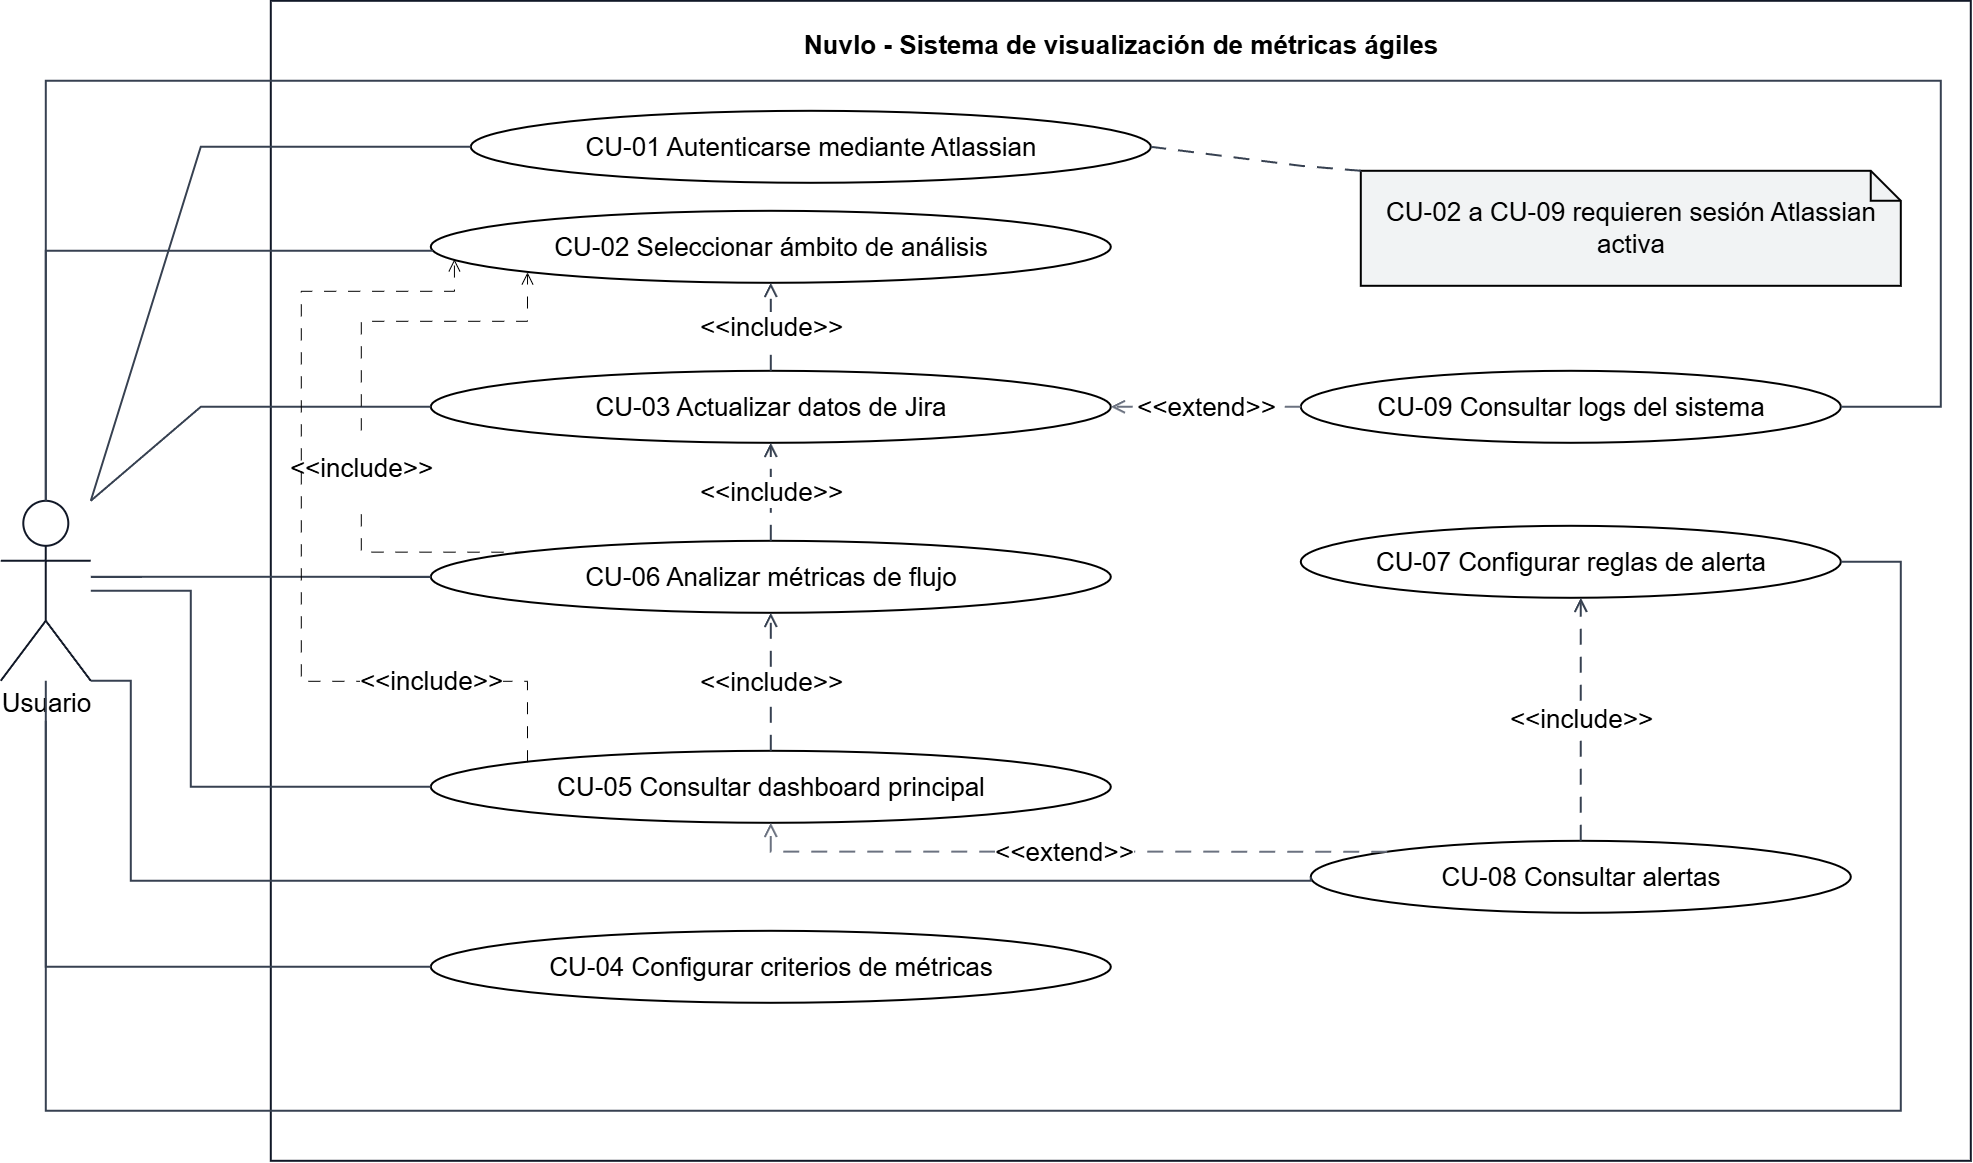
\includegraphics[width=\textwidth]{diagrams/casos-uso.png}
    \caption{Diagrama de casos de uso del sistema}
    \label{fig:casos-uso}
\end{figure}

Para facilitar su interpretación, se resumen a continuación los elementos principales del diagrama:

\begin{itemize}
    \item \textbf{Frontera del sistema}: el rectángulo delimita las funcionalidades que pertenecen al sistema de visualización de métricas ágiles.
    \item \textbf{Actores}: representan usuarios o sistemas externos que interactúan con el sistema.
    \item \textbf{Casos de uso}: las elipses identifican funcionalidades observables por los actores.
    \item \textbf{Generalización}: la flecha con triángulo hueco indica especialización entre actores.
    \item \textbf{Inclusión}: la relación \textit{include} indica que un caso de uso necesita ejecutar otro como parte de su comportamiento.
    \item \textbf{Extensión}: la relación \textit{extend} indica comportamiento opcional o condicionado que amplía otro caso de uso.
\end{itemize}

Los actores y sus relaciones principales son:

\begin{itemize}
    \item \textbf{Usuario}: actor general que puede iniciar el acceso al sistema mediante Atlassian.
    \item \textbf{Usuario autenticado}: especialización de \textit{Usuario}; puede seleccionar el ámbito de análisis, actualizar datos, consultar dashboards, analizar métricas, configurar reglas de alerta, consultar alertas y revisar logs.
    \item \textbf{Atlassian Cloud}: actor externo general que agrupa los servicios de Atlassian utilizados por el sistema.
    \item \textbf{Atlassian OAuth}: especialización de \textit{Atlassian Cloud}; participa en la autenticación mediante Atlassian.
    \item \textbf{Jira Cloud API}: especialización de \textit{Atlassian Cloud}; proporciona los datos de Jira necesarios para sincronización y cálculo de métricas.
\end{itemize}

Las relaciones entre casos de uso se interpretan de la siguiente forma:

\begin{itemize}
    \item \textbf{CU-05 incluye CU-02}: para consultar el dashboard principal es necesario seleccionar previamente el ámbito de análisis.
    \item \textbf{CU-06 incluye CU-02}: el análisis de métricas de flujo también depende del ámbito de análisis seleccionado.
    \item \textbf{CU-06 incluye CU-03}: para analizar métricas de flujo se requieren datos actualizados o previamente sincronizados desde Jira.
    \item \textbf{CU-08 incluye CU-07}: la consulta de alertas parte de reglas de alerta configuradas.
    \item \textbf{CU-08 extiende CU-05}: las alertas pueden complementar la consulta del dashboard cuando existan avisos relevantes.
    \item \textbf{CU-09 extiende CU-03}: los logs pueden consultarse como apoyo al diagnóstico de procesos de actualización, errores o eventos relevantes.
\end{itemize}

\clearpage
\section{Trazabilidad entre requisitos y casos de uso}

La trazabilidad permite comprobar que los casos de uso identificados cubren los requisitos funcionales principales. En esta fase inicial se plantea una matriz preliminar, que podrá ajustarse cuando se definan con mayor detalle los casos de uso y los diagramas asociados.

{\renewcommand{\arraystretch}{1.25}\scriptsize
\setlength{\tabcolsep}{3.2pt}
\begin{longtable}{|p{1.35cm}|c|c|c|c|c|c|c|c|c|}
\caption{Matriz de trazabilidad entre requisitos funcionales y casos de uso}\label{tab:trazabilidad-rf-cu}\\
\hline
\textbf{Req.} & \textbf{CU-01} & \textbf{CU-02} & \textbf{CU-03} & \textbf{CU-04} & \textbf{CU-05} & \textbf{CU-06} & \textbf{CU-07} & \textbf{CU-08} & \textbf{CU-09} \\
\hline
\endfirsthead
\hline
\textbf{Req.} & \textbf{CU-01} & \textbf{CU-02} & \textbf{CU-03} & \textbf{CU-04} & \textbf{CU-05} & \textbf{CU-06} & \textbf{CU-07} & \textbf{CU-08} & \textbf{CU-09} \\
\hline
\endhead
RF-01 &  &  & X &  &  &  &  &  &  \\\hline
RF-02 &  & X &  &  &  &  &  &  &  \\\hline
RF-03 &  &  & X &  &  &  &  &  &  \\\hline
RF-04 &  &  & X &  &  &  &  &  &  \\\hline
RF-05 &  &  & X &  &  &  &  &  &  \\\hline
RF-06 &  &  & X &  &  &  &  &  &  \\\hline
RF-07 &  & X &  & X &  &  &  &  &  \\\hline
RF-08 &  & X &  & X &  &  &  &  &  \\\hline
RF-09 &  &  &  &  & X & X &  &  &  \\\hline
RF-10 &  &  &  &  &  & X &  &  &  \\\hline
RF-11 &  &  & X &  &  &  &  &  &  \\\hline
RF-12 &  &  &  &  &  & X &  &  &  \\\hline
RF-13 &  &  &  &  &  & X &  &  &  \\\hline
RF-14 &  &  &  &  &  & X &  &  &  \\\hline
RF-15 &  &  &  &  &  & X &  &  &  \\\hline
RF-16 &  &  &  &  &  & X &  &  &  \\\hline
RF-17 &  &  &  &  &  & X &  &  &  \\\hline
RF-18 &  &  &  & X &  &  &  &  &  \\\hline
RF-19 &  &  &  &  & X &  &  &  &  \\\hline
RF-20 &  & X &  &  & X &  &  &  &  \\\hline
RF-21 &  &  &  &  & X &  &  &  &  \\\hline
RF-22 &  &  &  &  & X &  &  &  &  \\\hline
RF-23 &  &  &  &  & X &  &  &  &  \\\hline
RF-24 &  &  &  &  &  &  & X &  &  \\\hline
RF-25 &  &  &  &  &  &  &  & X &  \\\hline
RF-26 &  &  &  &  &  &  &  & X &  \\\hline
RF-27 &  &  &  &  &  &  &  &  & X \\\hline
RF-28 &  &  &  &  &  &  &  &  & X \\\hline
RF-29 & X &  &  &  &  &  &  &  &  \\\hline
RF-30 & X &  &  &  &  &  &  &  &  \\\hline
RF-31 & X &  &  &  &  &  &  &  &  \\\hline
\end{longtable}
\vspace{0.45em}
}

La matriz anterior no sustituye a la descripción detallada de los casos de uso. Su función es validar de forma visual que los requisitos funcionales quedan cubiertos por, al menos, un caso de uso identificado.
\clearpage
\section{Descripción detallada de los casos de uso}

Una vez identificados los casos de uso principales y validada su relación con los requisitos funcionales, se describen de forma detallada. Cada ficha recoge el actor principal, los actores secundarios, las precondiciones, el flujo principal, los posibles flujos alternativos, las postcondiciones y los requisitos relacionados. Esta descripción permite concretar el comportamiento esperado del sistema desde el punto de vista del usuario.

\subsection{CU-01: Autenticarse mediante Atlassian}

{\renewcommand{\arraystretch}{1.25}\footnotesize
\begin{longtable}{p{3.2cm}p{10.2cm}}
\toprule
\textbf{Campo} & \textbf{Descripción} \\
\midrule
\textbf{Actor principal} & Usuario. \\
\textbf{Actores secundarios} & Atlassian. \\
\textbf{Descripción} & Permite al usuario acceder al sistema utilizando el mecanismo oficial de autenticación de Atlassian, evitando el registro local de usuarios y el uso de credenciales propias de la aplicación. \\
\textbf{Precondiciones} & El usuario dispone de una cuenta válida de Atlassian. El servicio de autenticación de Atlassian está disponible. \\
\textbf{Flujo principal} & \begin{minipage}[t]{10.2cm}\begin{enumerate}[noitemsep,leftmargin=*]
    \item El usuario accede a la aplicación.
    \item El sistema muestra la opción de autenticación mediante Atlassian.
    \item El usuario selecciona iniciar sesión.
    \item El sistema redirige al usuario al mecanismo de autenticación de Atlassian.
    \item El usuario introduce sus credenciales en Atlassian y autoriza el acceso.
    \item Atlassian valida la autenticación y devuelve la respuesta al sistema.
    \item El sistema crea una sesión autenticada.
    \item El sistema muestra la pantalla principal de la aplicación.
\end{enumerate}\end{minipage} \\
\textbf{Flujos alternativos} & \begin{minipage}[t]{10.2cm}\begin{itemize}[noitemsep,leftmargin=*]
    \item El servicio de Atlassian no está disponible: el sistema informa de que no se puede completar la autenticación y el usuario permanece sin sesión iniciada.
    \item El usuario cancela el proceso de autenticación: el sistema vuelve a la pantalla inicial y no crea una sesión.
    \item La autenticación no es válida: el sistema informa de que no se ha podido iniciar sesión.
\end{itemize}\end{minipage} \\
\textbf{Postcondiciones} & El usuario queda autenticado en el sistema y puede acceder a las funcionalidades protegidas. \\
\textbf{Requisitos} & RF-29, RF-30, RF-31. \\
\bottomrule
\end{longtable}
\vspace{0.45em}
}

\clearpage
\subsection{CU-02: Seleccionar ámbito de análisis}

{\renewcommand{\arraystretch}{1.25}\footnotesize
\begin{longtable}{p{3.2cm}p{10.2cm}}
\toprule
\textbf{Campo} & \textbf{Descripción} \\
\midrule
\textbf{Actor principal} & Usuario autenticado. \\
\textbf{Actores secundarios} & Jira Cloud. \\
\textbf{Descripción} & Permite seleccionar el ámbito de datos sobre el que se desea trabajar, incluyendo proyecto, tablero, sprint, rango temporal, etiquetas, tipo de incidencia u otros criterios disponibles en Jira que se incorporen al sistema. \\
\textbf{Precondiciones} & El usuario ha iniciado sesión. El sistema dispone de conexión con Jira Cloud. Existen proyectos, tableros o datos disponibles para el usuario autenticado. \\
\textbf{Flujo principal} & \begin{minipage}[t]{10.2cm}\begin{enumerate}[noitemsep,leftmargin=*]
    \item El usuario accede a la sección de selección de ámbito.
    \item El sistema consulta los proyectos, tableros u opciones disponibles en Jira.
    \item El sistema muestra los criterios de selección disponibles.
    \item El usuario selecciona el proyecto, tablero, sprint, rango temporal u otros filtros.
    \item El sistema valida la selección realizada.
    \item El sistema guarda el ámbito de análisis seleccionado.
    \item El sistema actualiza las vistas o prepara la actualización de datos según el ámbito definido.
\end{enumerate}\end{minipage} \\
\textbf{Flujos alternativos} & \begin{minipage}[t]{10.2cm}\begin{itemize}[noitemsep,leftmargin=*]
    \item Jira Cloud no está disponible: el sistema informa de que no se pueden recuperar los datos y mantiene la selección anterior si existe.
    \item No existen proyectos o tableros disponibles: el sistema informa de que no se han encontrado ámbitos de análisis.
    \item La selección no es válida: el sistema informa del error y permite modificar los criterios seleccionados.
\end{itemize}\end{minipage} \\
\textbf{Postcondiciones} & El sistema dispone de un ámbito de análisis válido para actualizar datos, calcular métricas o filtrar visualizaciones. \\
\textbf{Requisitos} & RF-02, RF-07, RF-08, RF-20. \\
\bottomrule
\end{longtable}
\vspace{0.45em}
}

\clearpage
\subsection{CU-03: Actualizar datos de Jira}

{\renewcommand{\arraystretch}{1.25}\footnotesize
\begin{longtable}{p{3.2cm}p{10.2cm}}
\toprule
\textbf{Campo} & \textbf{Descripción} \\
\midrule
\textbf{Actor principal} & Usuario autenticado. \\
\textbf{Actores secundarios} & Jira Cloud. \\
\textbf{Descripción} & Permite actualizar los datos procedentes de Jira Cloud de forma controlada, reutilizando la información almacenada cuando siga siendo válida y evitando sincronizaciones completas innecesarias. \\
\textbf{Precondiciones} & El usuario ha iniciado sesión. Existe un ámbito de análisis seleccionado. La conexión con Jira Cloud está disponible cuando sea necesario consultar datos remotos. \\
\textbf{Flujo principal} & \begin{minipage}[t]{10.2cm}\begin{enumerate}[noitemsep,leftmargin=*]
    \item El usuario accede a un ámbito de análisis o solicita una actualización bajo demanda.
    \item El sistema comprueba la fecha de última actualización y el ámbito seleccionado.
    \item Si la información almacenada sigue siendo válida, el sistema reutiliza los datos disponibles.
    \item Si la información está desactualizada, el sistema consulta Jira Cloud API.
    \item El sistema importa o actualiza únicamente los datos necesarios cuando sea posible.
    \item El sistema registra la fecha y hora de actualización.
    \item El sistema detecta posibles datos incompletos o inconsistentes.
    \item El sistema recalcula las métricas afectadas.
    \item El sistema informa del estado de la actualización.
\end{enumerate}\end{minipage} \\
\textbf{Flujos alternativos} & \begin{minipage}[t]{10.2cm}\begin{itemize}[noitemsep,leftmargin=*]
    \item Jira Cloud no está disponible: el sistema informa del error, registra el evento y utiliza datos almacenados si existen.
    \item La API devuelve datos incompletos: el sistema registra la incidencia detectada y continúa con los datos válidos cuando sea posible.
    \item Se produce un error durante el cálculo de métricas: el sistema registra el error e informa de que la actualización se completó parcialmente.
\end{itemize}\end{minipage} \\
\textbf{Postcondiciones} & Los datos quedan actualizados o se reutilizan los datos almacenados válidos. Las métricas afectadas se recalculan cuando procede. \\
\textbf{Requisitos} & RF-01, RF-03, RF-04, RF-05, RF-06, RF-11. \\
\bottomrule
\end{longtable}
\vspace{0.45em}
}


\clearpage
\subsection{CU-04: Configurar criterios de cálculo de métricas}

{\renewcommand{\arraystretch}{1.25}\footnotesize
\begin{longtable}{p{3.2cm}p{10.2cm}}
\toprule
\textbf{Campo} & \textbf{Descripción} \\
\midrule
\textbf{Actor principal} & Usuario autenticado. \\
\textbf{Actores secundarios} & Ninguno. \\
\textbf{Descripción} & Permite definir cómo debe interpretar el sistema los datos procedentes de Jira para calcular métricas, incluyendo estados de inicio y fin, campo de esfuerzo, rango temporal, percentiles y criterios de agrupación. \\
\textbf{Precondiciones} & El usuario ha iniciado sesión. Existe un ámbito de análisis disponible. El sistema dispone de estados, campos o datos configurables. \\
\textbf{Flujo principal} & \begin{minipage}[t]{10.2cm}\begin{enumerate}[noitemsep,leftmargin=*]
    \item El usuario accede a la sección de configuración de criterios de cálculo.
    \item El sistema muestra los parámetros configurables según los datos disponibles.
    \item El usuario selecciona los estados que representan el inicio y el fin del trabajo efectivo.
    \item El usuario selecciona el campo de esfuerzo y otros criterios de análisis cuando proceda.
    \item El usuario ajusta percentiles, rango temporal o criterios de agrupación disponibles.
    \item El sistema valida la configuración introducida.
    \item El sistema guarda la configuración.
    \item El sistema aplica la configuración a los cálculos posteriores.
\end{enumerate}\end{minipage} \\
\textbf{Flujos alternativos} & \begin{minipage}[t]{10.2cm}\begin{itemize}[noitemsep,leftmargin=*]
    \item El usuario no selecciona estados válidos: el sistema informa del problema y solicita corregir la configuración.
    \item Algún parámetro es incompatible con los datos disponibles: el sistema informa del campo afectado y permite modificarlo.
    \item El usuario cancela la configuración: el sistema mantiene la configuración anterior.
\end{itemize}\end{minipage} \\
\textbf{Postcondiciones} & La configuración queda guardada y se utiliza para calcular las métricas del sistema. \\
\textbf{Requisitos} & RF-07, RF-08, RF-18. \\
\bottomrule
\end{longtable}
\vspace{0.45em}
}

\clearpage
\subsection{CU-05: Consultar dashboard principal}

{\renewcommand{\arraystretch}{1.25}\footnotesize
\begin{longtable}{p{3.2cm}p{10.2cm}}
\toprule
\textbf{Campo} & \textbf{Descripción} \\
\midrule
\textbf{Actor principal} & Usuario autenticado. \\
\textbf{Actores secundarios} & Ninguno. \\
\textbf{Descripción} & Permite visualizar en un dashboard principal las métricas clave del sistema para un periodo y ámbito de análisis seleccionados. \\
\textbf{Precondiciones} & El usuario ha iniciado sesión. Existe un ámbito de análisis seleccionado. El sistema dispone de datos sincronizados, almacenados o de demostración. \\
\textbf{Flujo principal} & \begin{minipage}[t]{10.2cm}\begin{enumerate}[noitemsep,leftmargin=*]
    \item El usuario accede al dashboard principal.
    \item El sistema obtiene las métricas disponibles para el ámbito seleccionado.
    \item El sistema muestra las métricas clave mediante widgets o visualizaciones.
    \item El usuario modifica filtros o rango temporal si lo desea.
    \item El sistema actualiza el dashboard según los filtros aplicados.
    \item El usuario consulta la información mostrada.
\end{enumerate}\end{minipage} \\
\textbf{Flujos alternativos} & \begin{minipage}[t]{10.2cm}\begin{itemize}[noitemsep,leftmargin=*]
    \item No existen datos disponibles: el sistema informa de la situación y puede mostrar datos de demostración si existen.
    \item Los filtros no devuelven resultados: el sistema informa de que no hay información para los criterios seleccionados.
\end{itemize}\end{minipage} \\
\textbf{Postcondiciones} & El usuario visualiza el estado general del proyecto o equipo mediante las métricas disponibles. \\
\textbf{Requisitos} & RF-09, RF-19, RF-20, RF-21, RF-22, RF-23. \\
\bottomrule
\end{longtable}
\vspace{0.45em}
}

\clearpage
\subsection{CU-06: Analizar métricas de flujo}

{\renewcommand{\arraystretch}{1.25}\footnotesize
\begin{longtable}{p{3.2cm}p{10.2cm}}
\toprule
\textbf{Campo} & \textbf{Descripción} \\
\midrule
\textbf{Actor principal} & Usuario autenticado. \\
\textbf{Actores secundarios} & Ninguno. \\
\textbf{Descripción} & Permite consultar métricas de flujo y rendimiento del equipo, como Velocity, WIP, Lead Time, Cycle Time y otras métricas adicionales cuando existan datos suficientes. \\
\textbf{Precondiciones} & El usuario ha iniciado sesión. El sistema dispone de datos sincronizados o almacenados. Los criterios necesarios para el cálculo de métricas están configurados. \\
\textbf{Flujo principal} & \begin{minipage}[t]{10.2cm}\begin{enumerate}[noitemsep,leftmargin=*]
    \item El usuario accede a la vista de análisis de métricas.
    \item El sistema muestra las métricas disponibles para el ámbito seleccionado.
    \item El usuario selecciona una métrica o conjunto de métricas.
    \item El sistema muestra los valores calculados y su evolución cuando proceda.
    \item El usuario aplica filtros o cambia el periodo de análisis.
    \item El sistema recalcula o actualiza la visualización.
    \item El usuario interpreta los resultados mostrados.
\end{enumerate}\end{minipage} \\
\textbf{Flujos alternativos} & \begin{minipage}[t]{10.2cm}\begin{itemize}[noitemsep,leftmargin=*]
    \item No existen datos suficientes para una métrica: el sistema informa de que la métrica no puede calcularse e indica, cuando sea posible, qué datos faltan.
    \item Se produce un error en el cálculo: el sistema registra el error e informa al usuario.
\end{itemize}\end{minipage} \\
\textbf{Postcondiciones} & El usuario dispone de información analítica sobre el flujo de trabajo y las métricas seleccionadas. \\
\textbf{Requisitos} & RF-09, RF-10, RF-12, RF-13, RF-14, RF-15, RF-16, RF-17. \\
\bottomrule
\end{longtable}
\vspace{0.45em}
}

\clearpage
\subsection{CU-07: Configurar reglas de alerta}

{\renewcommand{\arraystretch}{1.25}\footnotesize
\begin{longtable}{p{3.2cm}p{10.2cm}}
\toprule
\textbf{Campo} & \textbf{Descripción} \\
\midrule
\textbf{Actor principal} & Usuario autenticado. \\
\textbf{Actores secundarios} & Ninguno. \\
\textbf{Descripción} & Permite definir reglas de alerta simples basadas en umbrales configurables sobre métricas calculadas, como WIP, Cycle Time, Lead Time o Velocity. \\
\textbf{Precondiciones} & El usuario ha iniciado sesión. El sistema dispone de métricas calculadas o configurables. El usuario conoce el umbral que desea establecer. \\
\textbf{Flujo principal} & \begin{minipage}[t]{10.2cm}\begin{enumerate}[noitemsep,leftmargin=*]
    \item El usuario accede a la sección de configuración de alertas.
    \item El sistema muestra las métricas disponibles para crear reglas.
    \item El usuario selecciona la métrica sobre la que quiere definir una alerta.
    \item El usuario introduce el umbral o condición simple.
    \item El usuario guarda la regla de alerta.
    \item El sistema valida la regla introducida.
    \item El sistema almacena la regla.
    \item El sistema evalúa la regla cuando se actualicen las métricas.
\end{enumerate}\end{minipage} \\
\textbf{Flujos alternativos} & \begin{minipage}[t]{10.2cm}\begin{itemize}[noitemsep,leftmargin=*]
    \item El usuario introduce un umbral no válido: el sistema informa del error y solicita corregir el valor.
    \item La regla no puede aplicarse a la métrica seleccionada: el sistema informa de la incompatibilidad y permite modificar la regla.
\end{itemize}\end{minipage} \\
\textbf{Postcondiciones} & La regla de alerta queda registrada y podrá activarse cuando se cumpla la condición definida. \\
\textbf{Requisitos} & RF-24. \\
\bottomrule
\end{longtable}
\vspace{0.45em}
}

\clearpage
\subsection{CU-08: Consultar alertas}

{\renewcommand{\arraystretch}{1.25}\footnotesize
\begin{longtable}{p{3.2cm}p{10.2cm}}
\toprule
\textbf{Campo} & \textbf{Descripción} \\
\midrule
\textbf{Actor principal} & Usuario autenticado. \\
\textbf{Actores secundarios} & Ninguno. \\
\textbf{Descripción} & Permite consultar alertas activas e históricas conservadas por el sistema, incluyendo su estado, momento de activación, métrica asociada y periodo de disponibilidad. \\
\textbf{Precondiciones} & El usuario ha iniciado sesión. Existen reglas de alerta configuradas. El sistema ha evaluado las métricas disponibles. \\
\textbf{Flujo principal} & \begin{minipage}[t]{10.2cm}\begin{enumerate}[noitemsep,leftmargin=*]
    \item El usuario accede a la sección de alertas.
    \item El sistema muestra las alertas activas e históricas conservadas.
    \item El usuario filtra las alertas por estado, métrica o periodo si lo desea.
    \item El sistema actualiza la lista de alertas según los filtros aplicados.
    \item El usuario consulta el detalle de una alerta.
\end{enumerate}\end{minipage} \\
\textbf{Flujos alternativos} & \begin{minipage}[t]{10.2cm}\begin{itemize}[noitemsep,leftmargin=*]
    \item No existen alertas registradas: el sistema informa de que no hay alertas disponibles.
    \item Los filtros no devuelven resultados: el sistema informa de que no existen alertas para los criterios seleccionados.
    \item La alerta histórica ha expirado según la política de retención: el sistema no la muestra en la consulta ordinaria.
\end{itemize}\end{minipage} \\
\textbf{Postcondiciones} & El usuario visualiza las alertas relevantes disponibles según los filtros aplicados y la política de retención definida. \\
\textbf{Requisitos} & RF-25, RF-26. \\
\bottomrule
\end{longtable}
\vspace{0.45em}
}

\clearpage
\subsection{CU-09: Consultar logs del sistema}

{\renewcommand{\arraystretch}{1.25}\footnotesize
\begin{longtable}{p{3.2cm}p{10.2cm}}
\toprule
\textbf{Campo} & \textbf{Descripción} \\
\midrule
\textbf{Actor principal} & Usuario autenticado. \\
\textbf{Actores secundarios} & Ninguno. \\
\textbf{Descripción} & Permite consultar eventos relevantes generados por el sistema, como actualizaciones de datos, errores de integración, errores de cálculo o eventos de autenticación asociados al uso de la aplicación. \\
\textbf{Precondiciones} & El usuario ha iniciado sesión. Existen eventos registrados por el sistema. \\
\textbf{Flujo principal} & \begin{minipage}[t]{10.2cm}\begin{enumerate}[noitemsep,leftmargin=*]
    \item El usuario accede a la sección de logs.
    \item El sistema muestra una lista de eventos registrados.
    \item El usuario aplica filtros básicos si lo considera necesario.
    \item El sistema actualiza la lista según los criterios seleccionados.
    \item El usuario consulta el detalle de un evento concreto.
\end{enumerate}\end{minipage} \\
\textbf{Flujos alternativos} & \begin{minipage}[t]{10.2cm}\begin{itemize}[noitemsep,leftmargin=*]
    \item No existen logs disponibles: el sistema informa de que no hay eventos registrados.
    \item No hay resultados para los filtros aplicados: el sistema muestra un mensaje indicando que no se han encontrado eventos.
    \item Algunos logs han expirado según la política de retención: el sistema no los muestra en la consulta ordinaria.
\end{itemize}\end{minipage} \\
\textbf{Postcondiciones} & El usuario visualiza los eventos relevantes disponibles según los filtros aplicados y la política de retención definida. \\
\textbf{Requisitos} & RF-27, RF-28. \\
\bottomrule
\end{longtable}
\vspace{0.45em}
}

\clearpage
\section{Diagramas de secuencia}

Los diagramas de secuencia complementan la descripción textual de los casos de uso mostrando el orden temporal de los mensajes intercambiados entre el usuario, la aplicación y los servicios externos. En esta memoria se incluyen únicamente los casos de uso más representativos, ya que son los que concentran la interacción con Atlassian, Jira Cloud API y la lógica principal del sistema.

\subsection{CU-01: Autenticarse mediante Atlassian}

Este diagrama de secuencia describe el comportamiento asociado al caso de uso CU-01, centrado en el inicio de sesión del usuario mediante el proveedor de autenticación de Atlassian.

\begin{figure}[htbp]
    \centering
    \makebox[\textwidth][c]{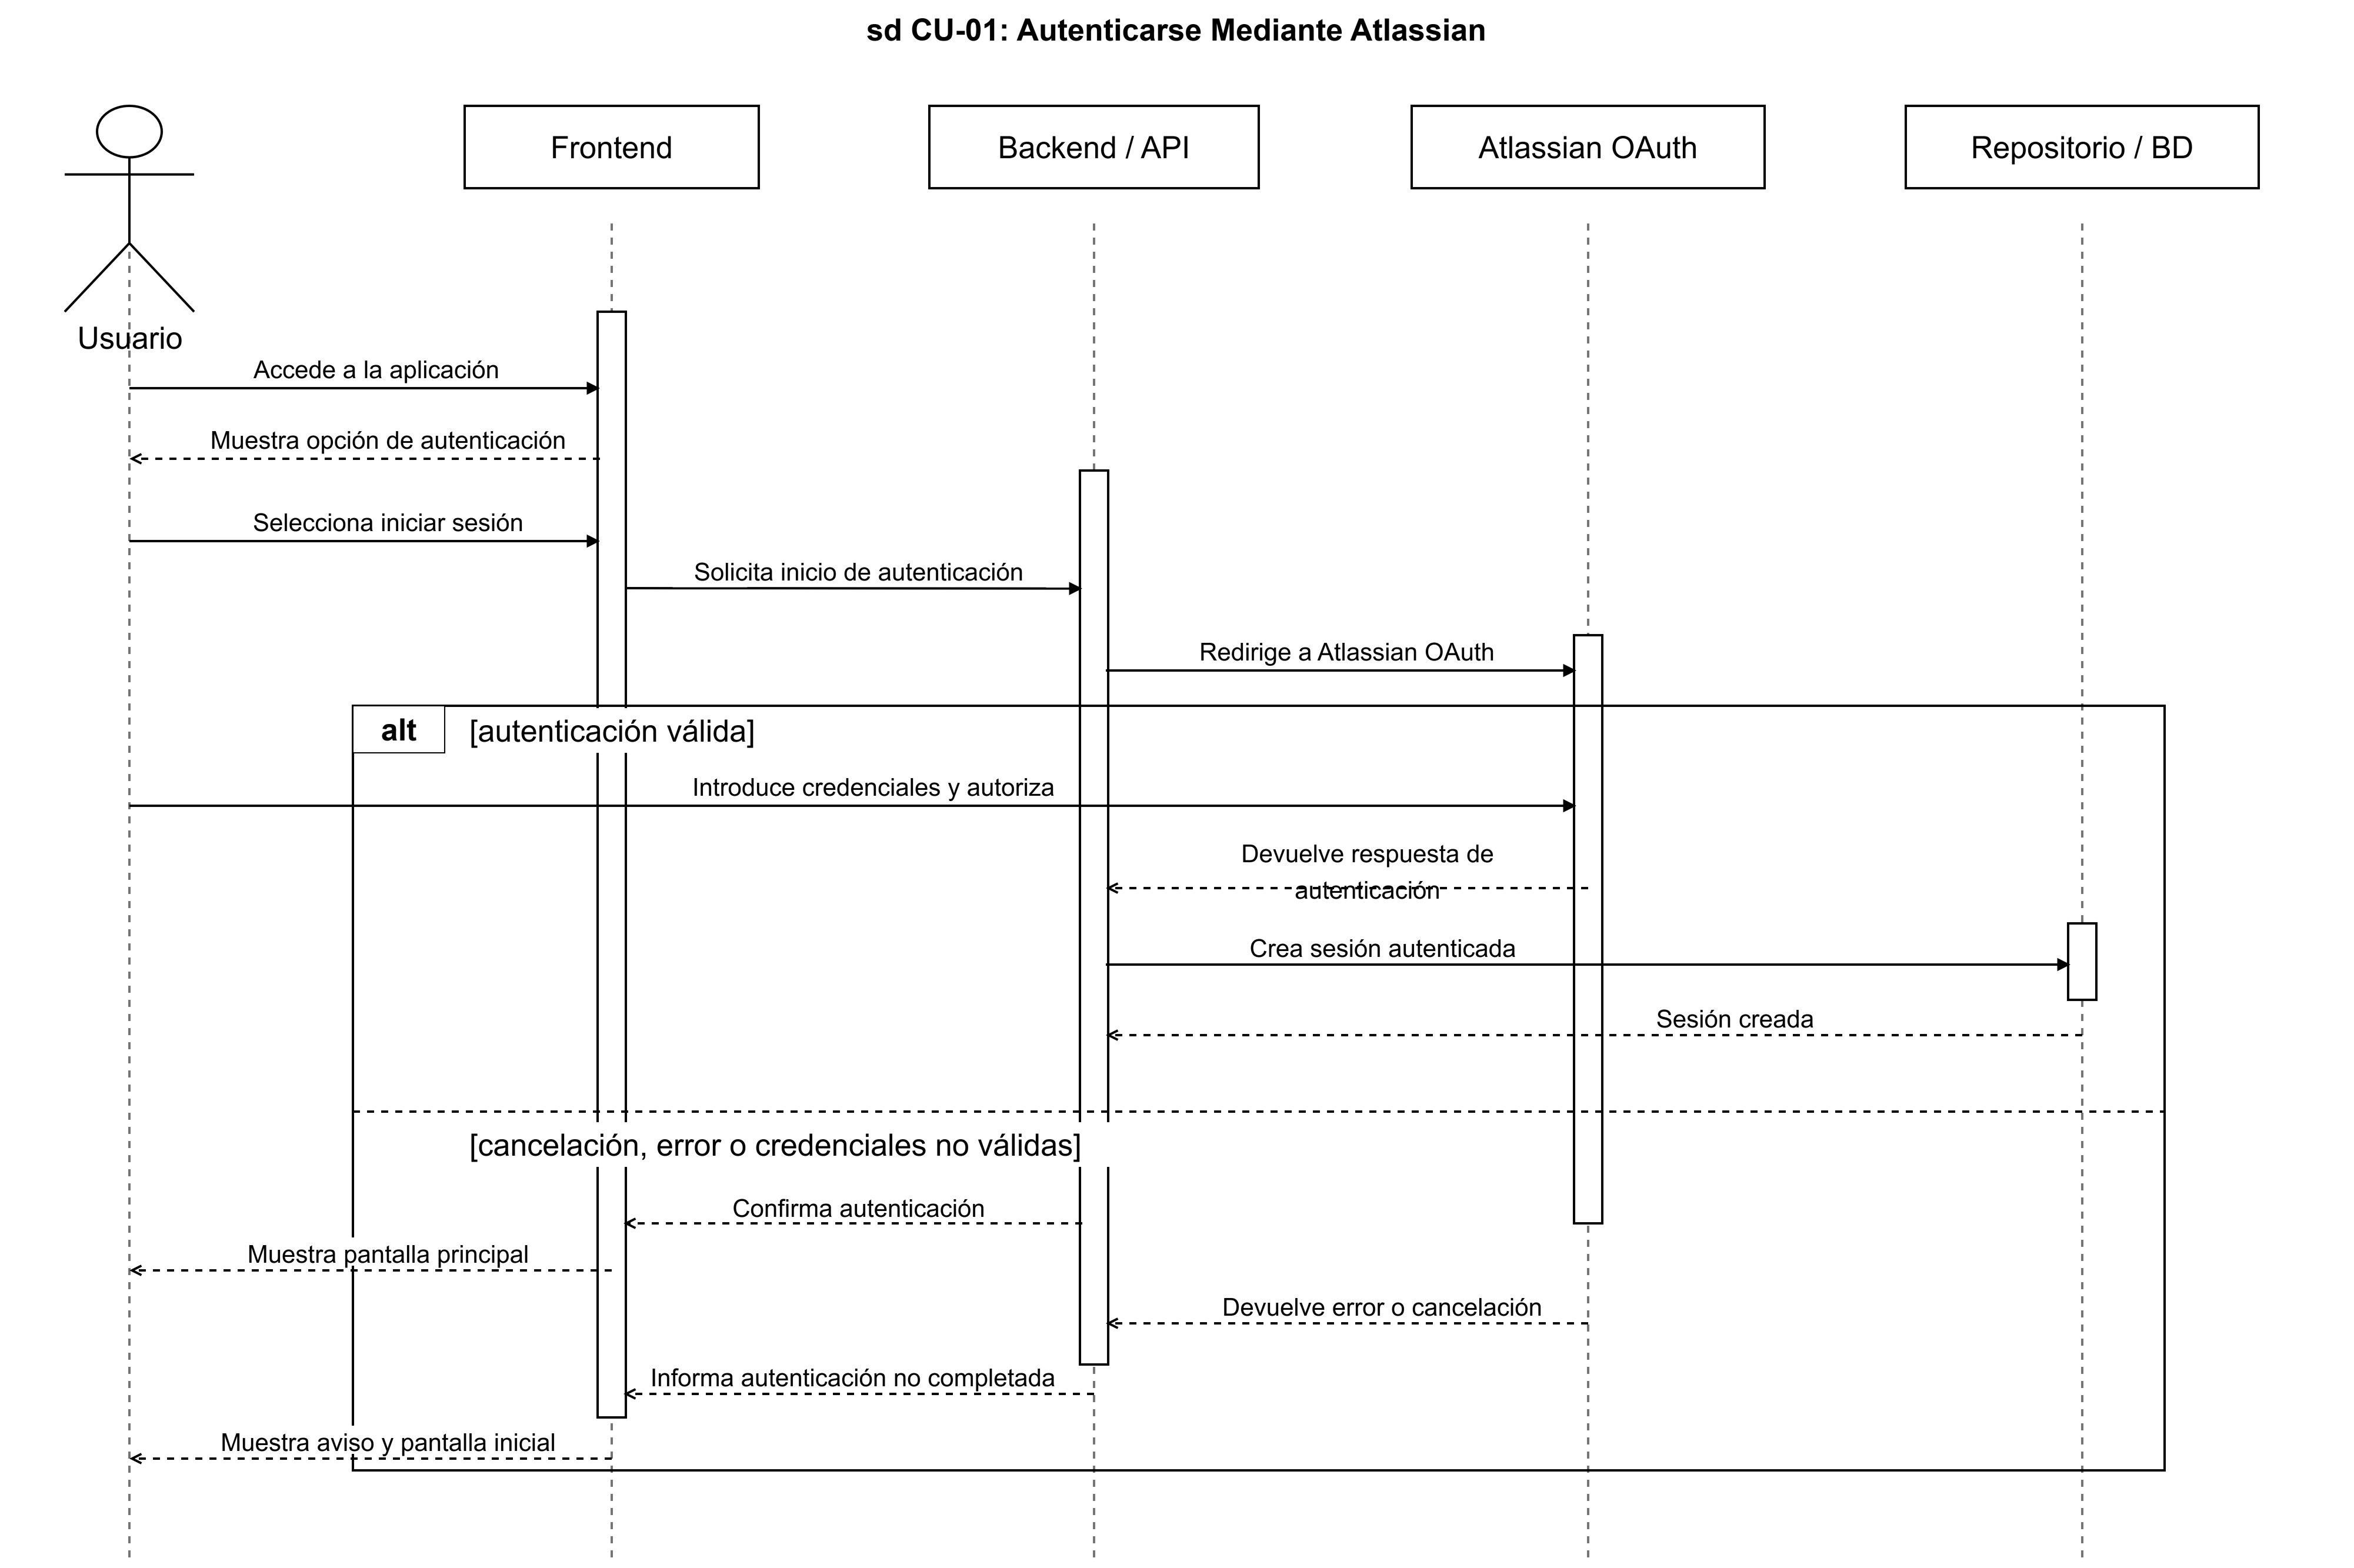
\includegraphics[width=1.08\textwidth]{diagrams/secuencia-cu01-autenticarse-atlassian.png}}
    \caption{Diagrama de secuencia del caso de uso CU-01}
    \label{fig:secuencia-cu01-autenticarse-atlassian}
\end{figure}

La Figura~\ref{fig:secuencia-cu01-autenticarse-atlassian} representa el proceso de autenticación mediante Atlassian. El usuario inicia sesión desde la aplicación, el sistema redirige la operación hacia Atlassian OAuth y, si la autenticación es válida, se crea una sesión autenticada. También se contempla el caso alternativo en el que el usuario cancela el proceso o Atlassian devuelve un error.

\subsection{CU-03: Actualizar datos de Jira}

Este diagrama de secuencia describe el comportamiento asociado al caso de uso CU-03, correspondiente a la actualización de la información procedente de Jira y al tratamiento posterior de los datos obtenidos.

\begin{figure}[htbp]
    \centering
    \makebox[\textwidth][c]{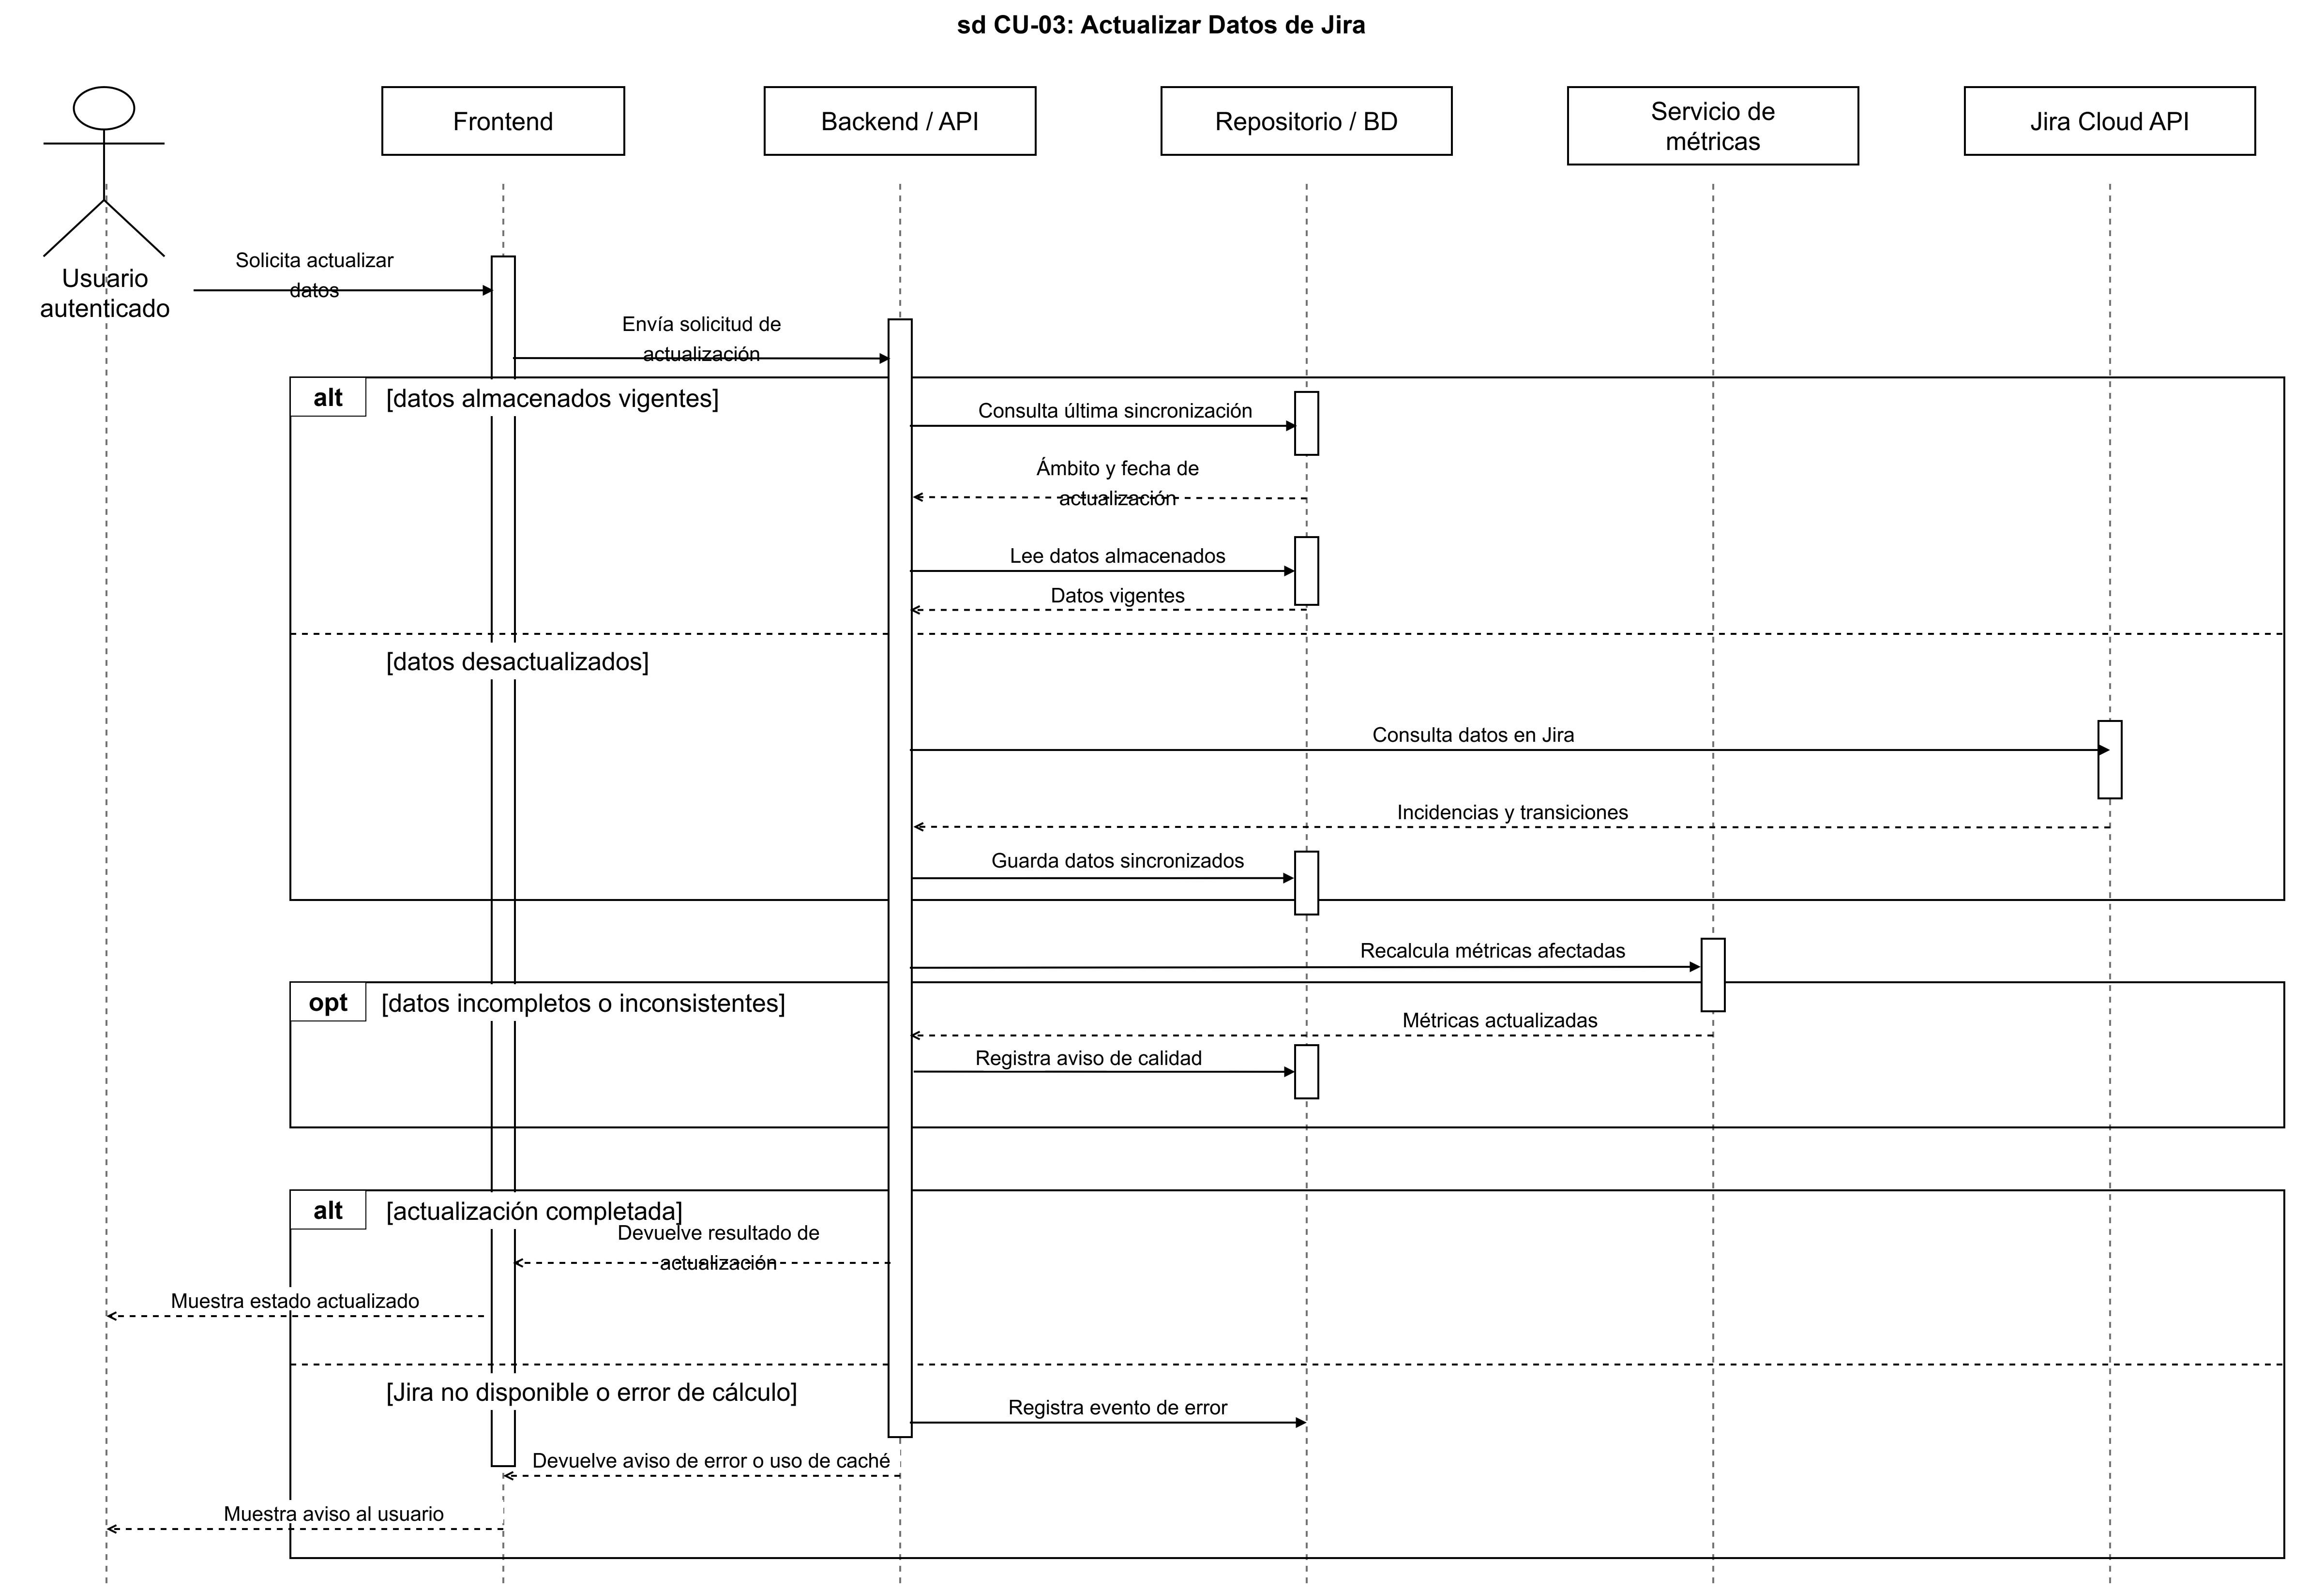
\includegraphics[width=1.08\textwidth]{diagrams/secuencia-cu03-actualizar-datos-jira.png}}
    \caption{Diagrama de secuencia del caso de uso CU-03}
    \label{fig:secuencia-cu03-actualizar-datos-jira}
\end{figure}

La Figura~\ref{fig:secuencia-cu03-actualizar-datos-jira} resume la actualización de datos desde Jira. El usuario autenticado solicita la actualización, el sistema comprueba si los datos almacenados siguen siendo válidos y, en caso contrario, consulta Jira Cloud API. A continuación, persiste la información obtenida, recalcula las métricas afectadas y comunica el resultado, contemplando también situaciones de error o datos incompletos.

\newpage

\subsection{CU-05: Consultar dashboard principal}

Este diagrama de secuencia describe el comportamiento asociado al caso de uso CU-05, centrado en la visualización del dashboard principal para un ámbito de análisis y unos filtros determinados.

\begin{figure}[htbp]
    \centering
    \makebox[\textwidth][c]{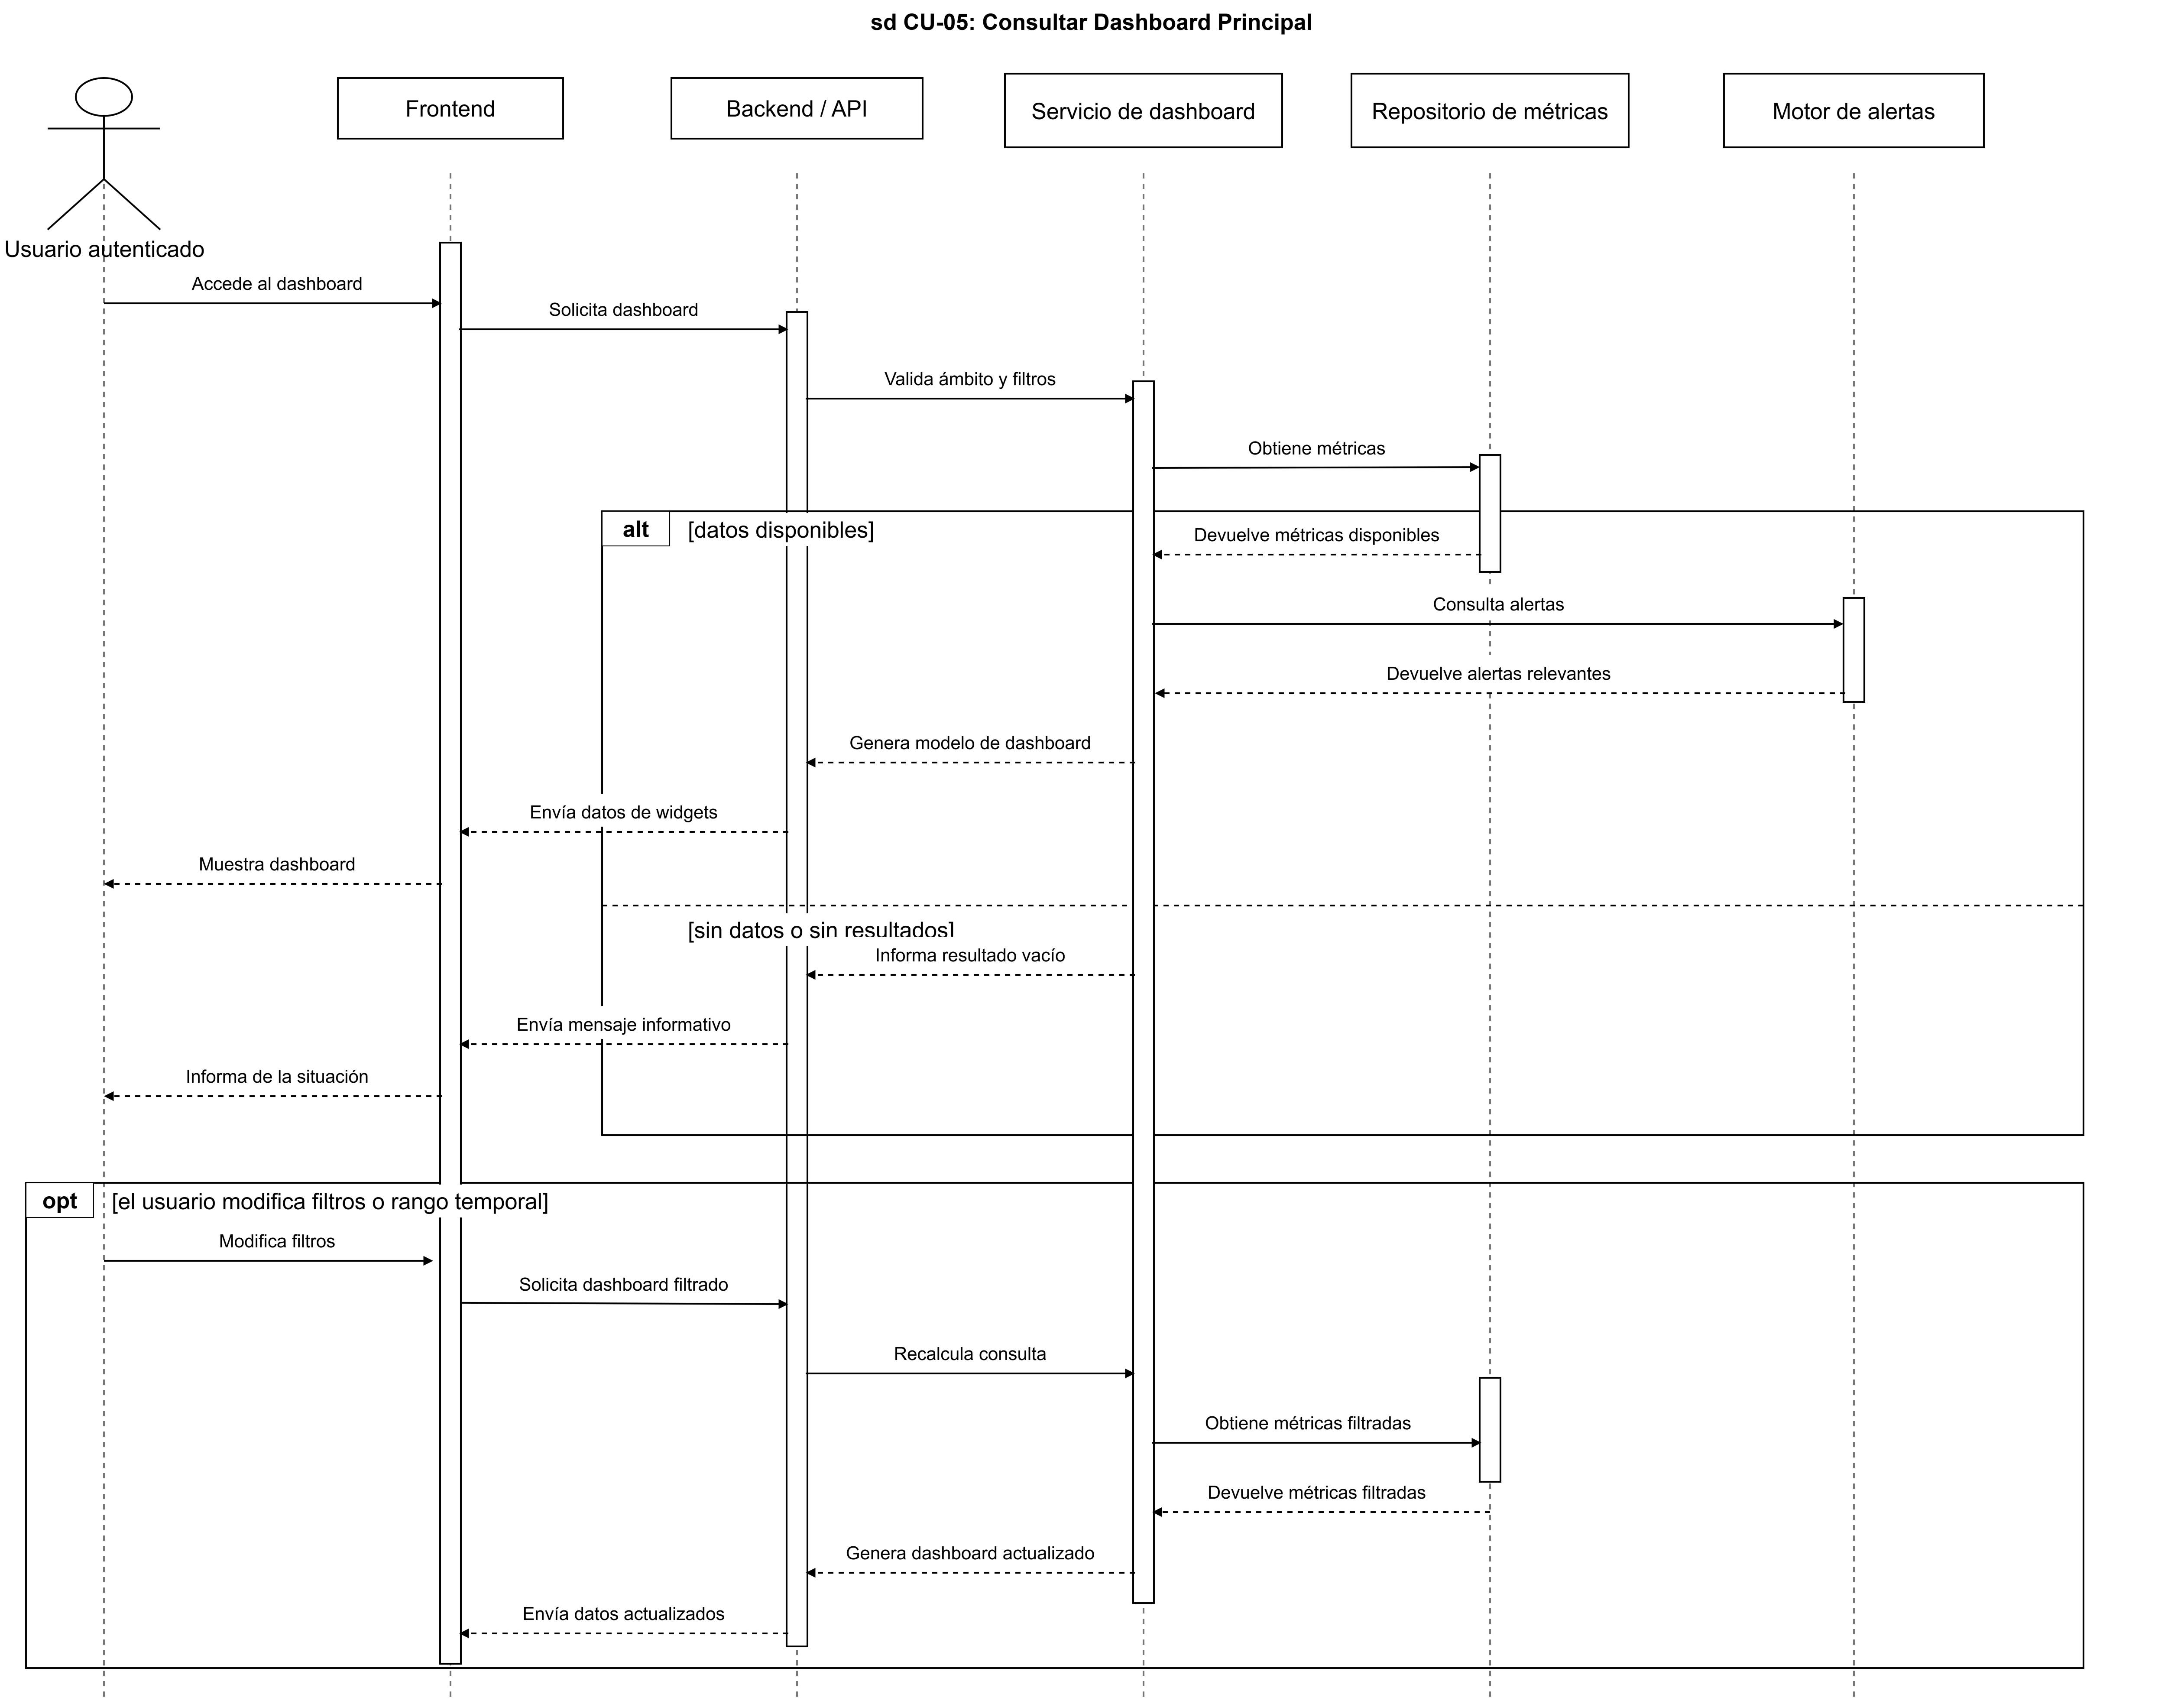
\includegraphics[width=1.08\textwidth]{diagrams/secuencia-cu05-consultar-dashboard-principal.png}}
    \caption{Diagrama de secuencia del caso de uso CU-05}
    \label{fig:secuencia-cu05-consultar-dashboard-principal}
\end{figure}

La Figura~\ref{fig:secuencia-cu05-consultar-dashboard-principal} muestra cómo el usuario autenticado accede al dashboard, el frontend solicita los datos al backend y el sistema valida el ámbito y los filtros antes de recuperar las métricas disponibles. El diagrama contempla la respuesta normal con los datos necesarios para construir los widgets, el caso alternativo en el que no existen datos o los filtros no devuelven resultados, y la actualización del dashboard cuando el usuario modifica los filtros o el rango temporal.

\subsection{CU-06: Analizar métricas de flujo}

Este diagrama de secuencia describe el comportamiento asociado al caso de uso CU-06, centrado en la consulta de métricas de flujo y rendimiento a partir de los datos sincronizados y los criterios de cálculo configurados.

\begin{figure}[htbp]
    \centering
    \makebox[\textwidth][c]{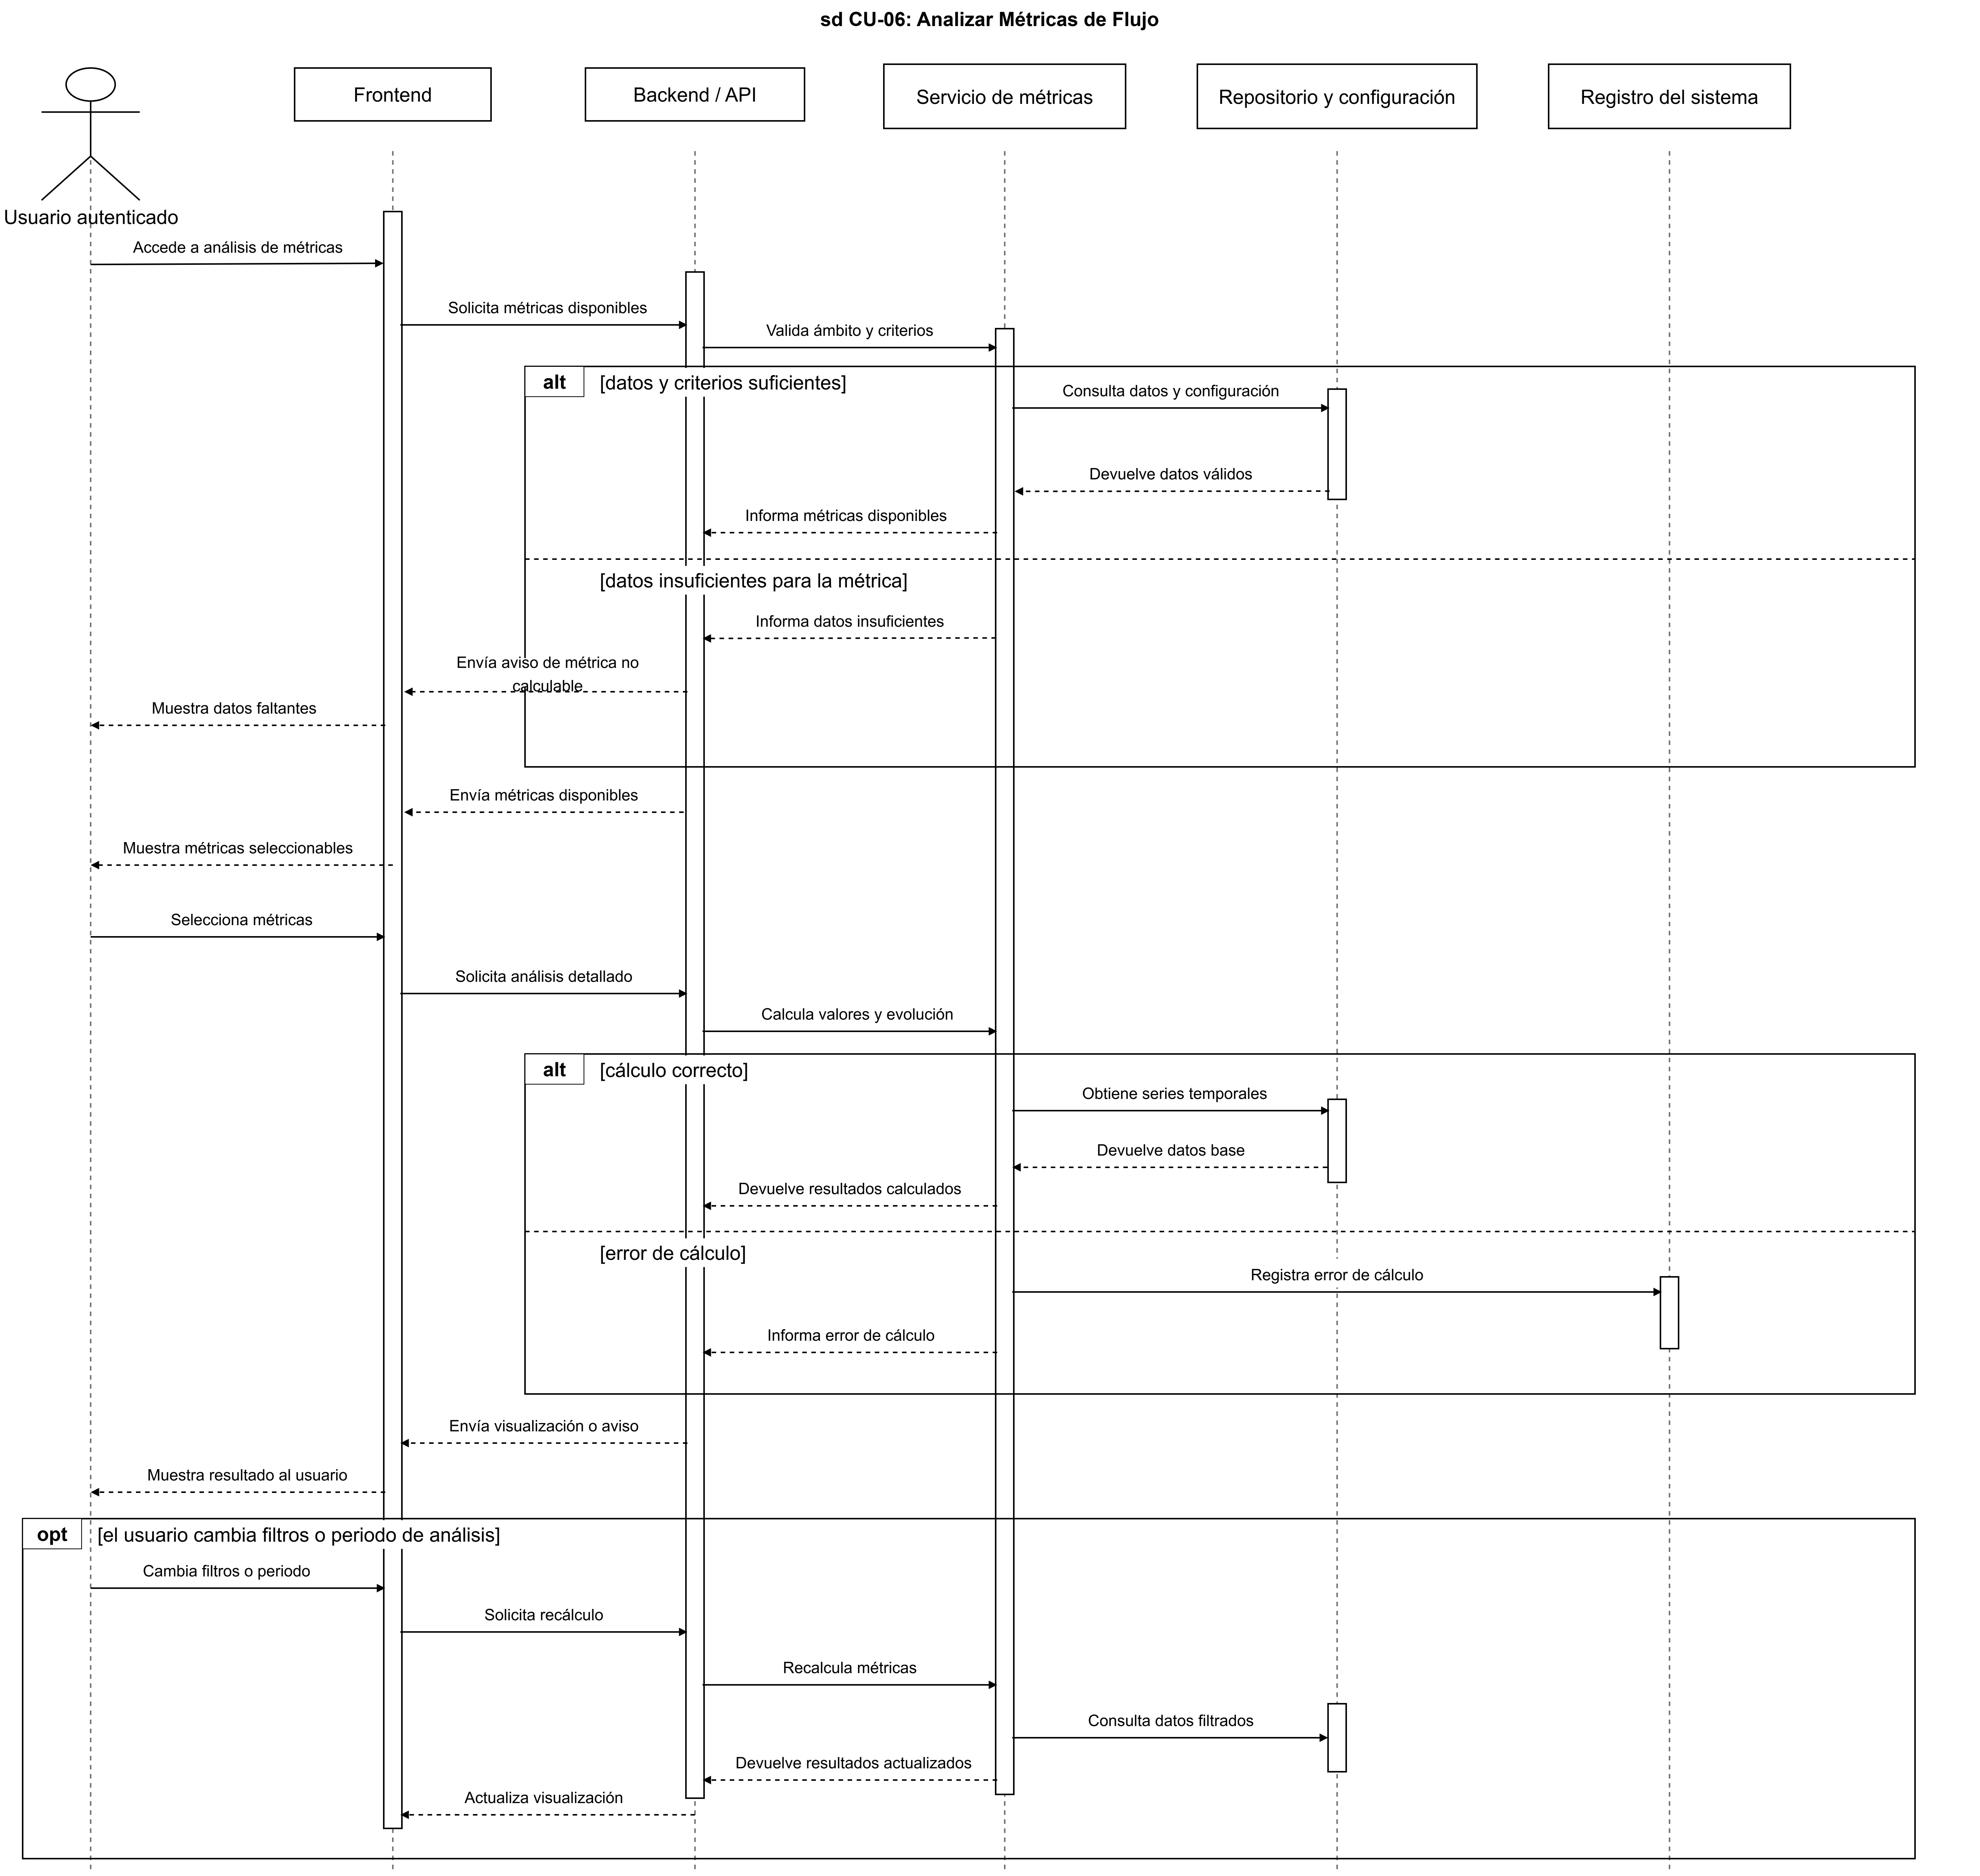
\includegraphics[width=1.08\textwidth]{diagrams/secuencia-cu06-analizar-metricas-flujo.png}}
    \caption{Diagrama de secuencia del caso de uso CU-06}
    \label{fig:secuencia-cu06-analizar-metricas-flujo}
\end{figure}

La Figura~\ref{fig:secuencia-cu06-analizar-metricas-flujo} muestra cómo el usuario autenticado accede a la vista de análisis, el sistema valida el ámbito seleccionado y recupera los datos y criterios necesarios para calcular las métricas disponibles. El diagrama contempla el flujo normal de selección y cálculo de métricas, el caso alternativo en el que no existen datos suficientes, el registro de errores de cálculo y la actualización de resultados cuando el usuario modifica filtros o el periodo de análisis.

\newpage

\subsection{CU-07: Configurar reglas de alerta}

Este diagrama de secuencia describe el comportamiento asociado al caso de uso CU-07, centrado en la creación de reglas de alerta a partir de métricas disponibles y condiciones simples definidas por el usuario.

\begin{figure}[htbp]
    \centering
    \makebox[\textwidth][c]{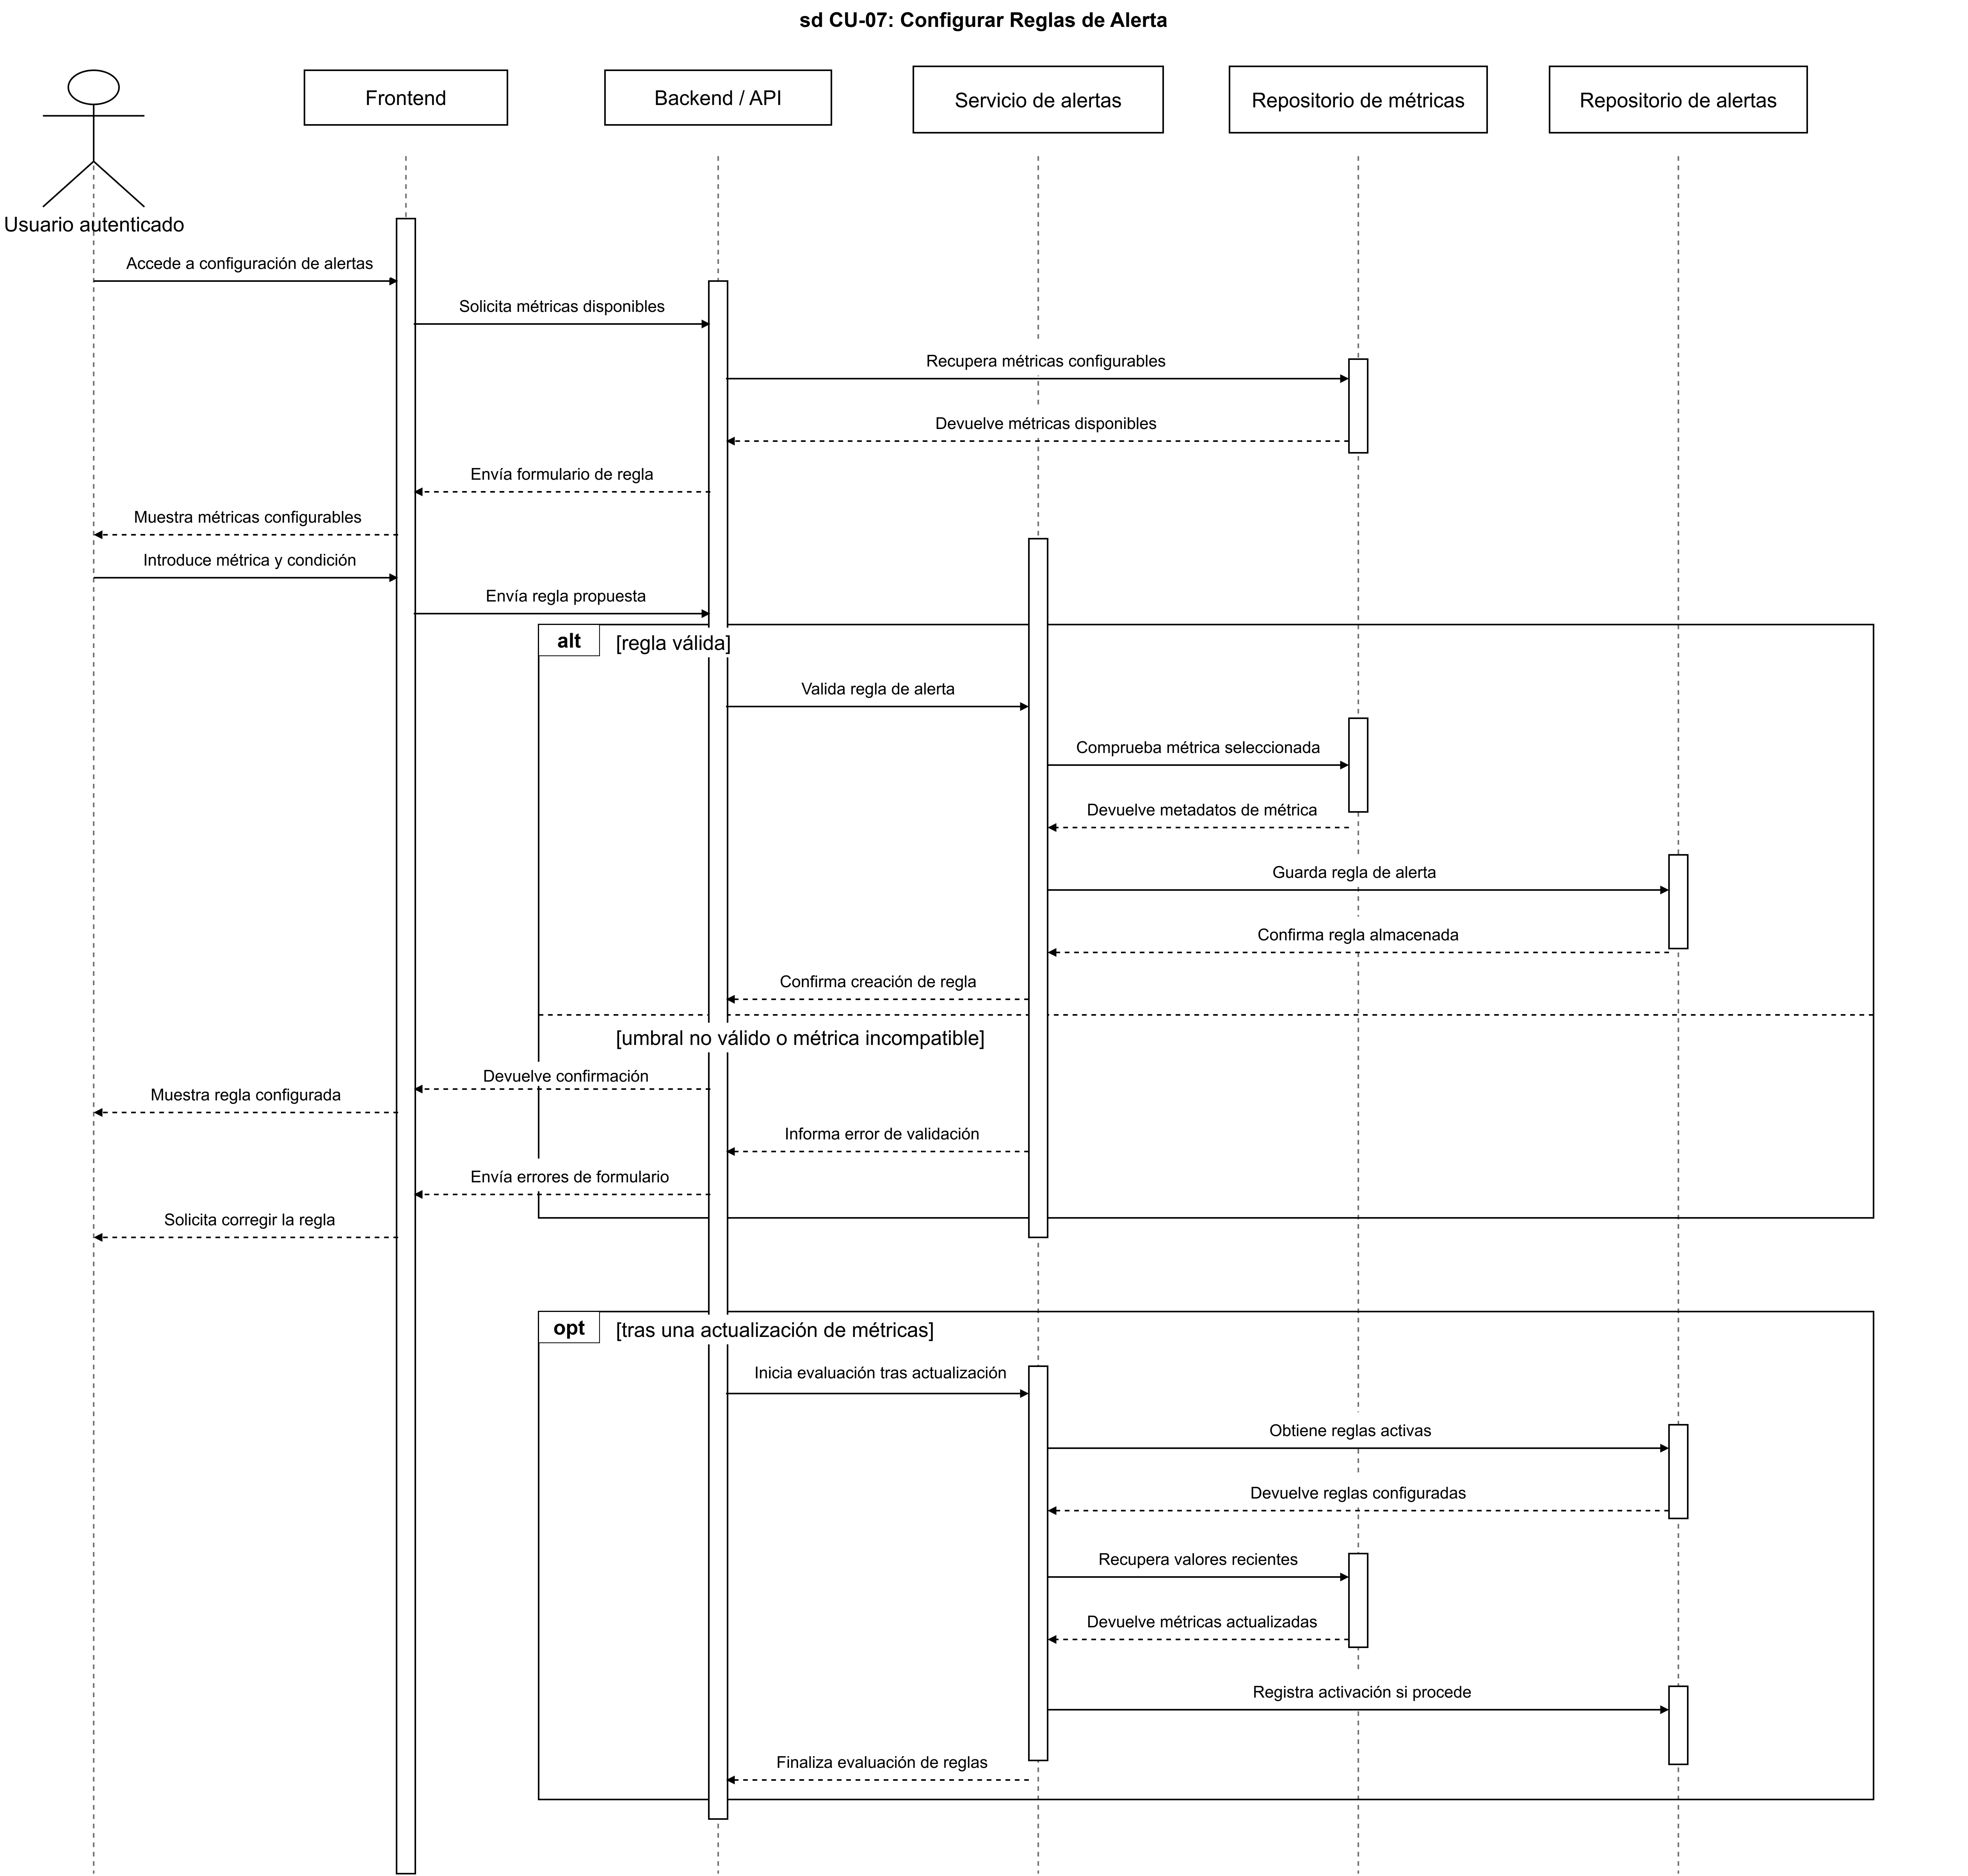
\includegraphics[width=1.08\textwidth]{diagrams/secuencia-cu07-configurar-reglas-alerta.png}}
    \caption{Diagrama de secuencia del caso de uso CU-07}
    \label{fig:secuencia-cu07-configurar-reglas-alerta}
\end{figure}

La Figura~\ref{fig:secuencia-cu07-configurar-reglas-alerta} muestra cómo el usuario autenticado accede a la configuración de alertas, selecciona una métrica y define una condición o umbral. El sistema valida la regla propuesta, comprueba que sea compatible con la métrica seleccionada y la almacena para que pueda evaluarse posteriormente cuando se actualicen las métricas. También se contempla el caso alternativo en el que la regla no es válida o no puede aplicarse a la métrica elegida.
\clearpage
\section{Diagrama de clases}

El diagrama de clases muestra la estructura estática principal del sistema y las relaciones entre los conceptos del dominio. En este caso se representa una vista de análisis previa a la implementación, por lo que las clases describen entidades y responsabilidades del sistema sin depender de una tecnología concreta.

\begin{figure}[htbp]
    \centering
    \makebox[\textwidth][c]{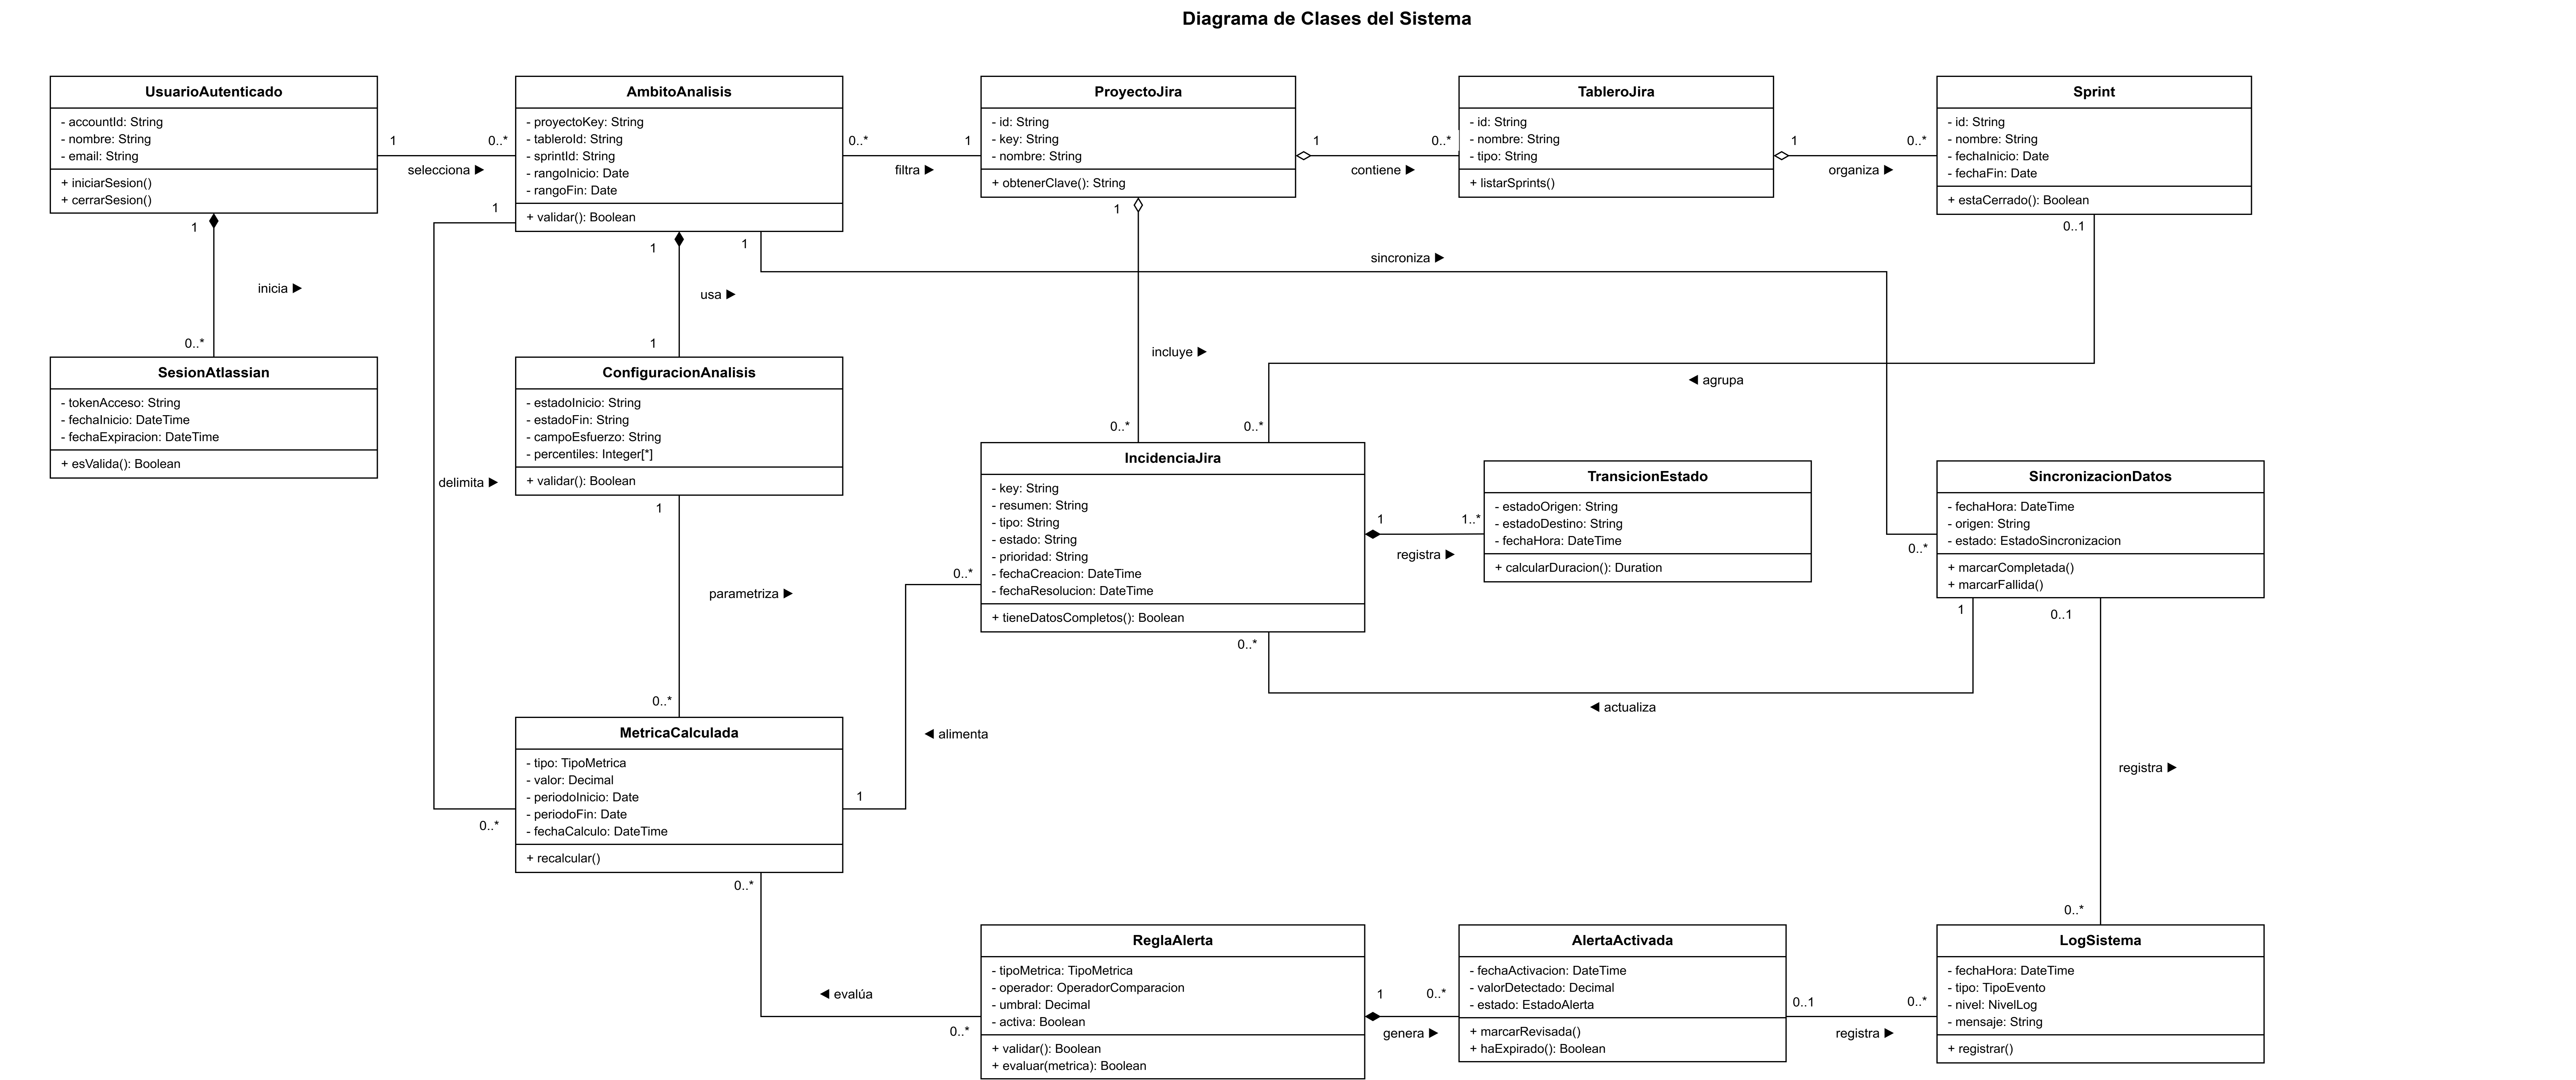
\includegraphics[width=1.25\textwidth]{diagrams/clases-dominio-sistema.png}}
    \caption{Diagrama de clases del sistema}
    \label{fig:clases-dominio-sistema}
\end{figure}

La Figura~\ref{fig:clases-dominio-sistema} se interpreta a partir de los verbos situados sobre cada relación. El triángulo del verbo indica la dirección de lectura y las cardinalidades de los extremos concretan cuántas instancias pueden participar en cada asociación. En cuanto a la notación UML, según la especificación oficial de OMG \cite{OMGUML251}, el rombo blanco representa una agregación, es decir, una relación todo-parte débil en la que la parte puede existir de forma independiente. El rombo negro representa una composición, una relación todo-parte fuerte en la que la parte depende del ciclo de vida del todo. Las clases del diagrama son las siguientes:

\begin{itemize}
    \item \texttt{UsuarioAutenticado}: representa al usuario que accede al sistema. Inicia sesiones de Atlassian y selecciona los ámbitos de análisis sobre los que desea trabajar.
    \item \texttt{SesionAtlassian}: recoge la sesión iniciada mediante Atlassian. Queda asociada al usuario autenticado que la ha creado.
    \item \texttt{AmbitoAnalisis}: define el alcance funcional del análisis. Usa una configuración de análisis, filtra proyectos de Jira, sincroniza datos y delimita las métricas calculadas.
    \item \texttt{ConfiguracionAnalisis}: contiene los criterios de cálculo, filtros y parámetros seleccionados por el usuario. Parametriza las métricas calculadas que se obtienen para un ámbito.
    \item \texttt{ProyectoJira}: representa un proyecto procedente de Jira. Es filtrado por el ámbito de análisis, contiene tableros e incluye incidencias.
    \item \texttt{TableroJira}: modela un tablero de trabajo de Jira. Pertenece a un proyecto y organiza los sprints utilizados en el análisis.
    \item \texttt{Sprint}: representa una iteración de trabajo. Está organizado por un tablero y agrupa las incidencias planificadas o revisadas durante ese periodo.
    \item \texttt{IncidenciaJira}: modela una tarea, historia, error u otro elemento importado desde Jira. Pertenece al proyecto, puede estar agrupada en un sprint, registra transiciones de estado, es actualizada por la sincronización y alimenta el cálculo de métricas.
    \item \texttt{TransicionEstado}: representa un cambio de estado de una incidencia. Queda registrada por la incidencia a la que pertenece y permite analizar tiempos de flujo.
    \item \texttt{SincronizacionDatos}: representa el proceso de actualización de información desde Jira. Se ejecuta dentro de un ámbito de análisis, actualiza incidencias y registra eventos en el log del sistema.
    \item \texttt{MetricaCalculada}: almacena el resultado de aplicar los criterios de análisis. Está parametrizada por la configuración, delimitada por el ámbito y alimentada por las incidencias; además, puede ser evaluada por reglas de alerta.
    \item \texttt{ReglaAlerta}: define una condición o umbral configurable. Evalúa métricas calculadas y genera alertas cuando se cumplen sus condiciones.
    \item \texttt{AlertaActivada}: representa una alerta producida por una regla. Se genera a partir de una regla de alerta y registra su aparición en el log del sistema.
    \item \texttt{LogSistema}: recoge eventos relevantes del sistema. Registra tanto procesos de sincronización como alertas activadas para facilitar la trazabilidad.
\end{itemize}

\clearpage
\section{Diagrama entidad-relación de la base de datos}

El diagrama entidad-relación describe la estructura lógica prevista para la persistencia del sistema. A diferencia del diagrama de clases, que representa conceptos del dominio y responsabilidades de análisis, este modelo se centra en tablas, claves primarias, claves foráneas y cardinalidades. Para facilitar su lectura se emplean entidades rectangulares con sus atributos internos y relaciones representadas mediante rombos, siguiendo la forma habitual de los diagramas entidad-relación y las formas disponibles en draw.io para modelos de bases de datos~\cite{DrawioERTables}. Cada rombo contiene un verbo que describe la relación y las cardinalidades se sitúan junto a los extremos conectados. Los nombres de tablas y columnas se han planteado en minúsculas y con \texttt{snake\_case}, siguiendo criterios habituales de estilo SQL~\cite{HolywellSQLStyle}; además, se evitan estructuras innecesariamente complejas para mantener un diseño comprensible y normalizado, de acuerdo con las recomendaciones generales de diseño relacional recogidas por Karwin~\cite{Karwin2010SQLAntipatterns}.

\begin{figure}[htbp]
    \centering
    \makebox[\textwidth][c]{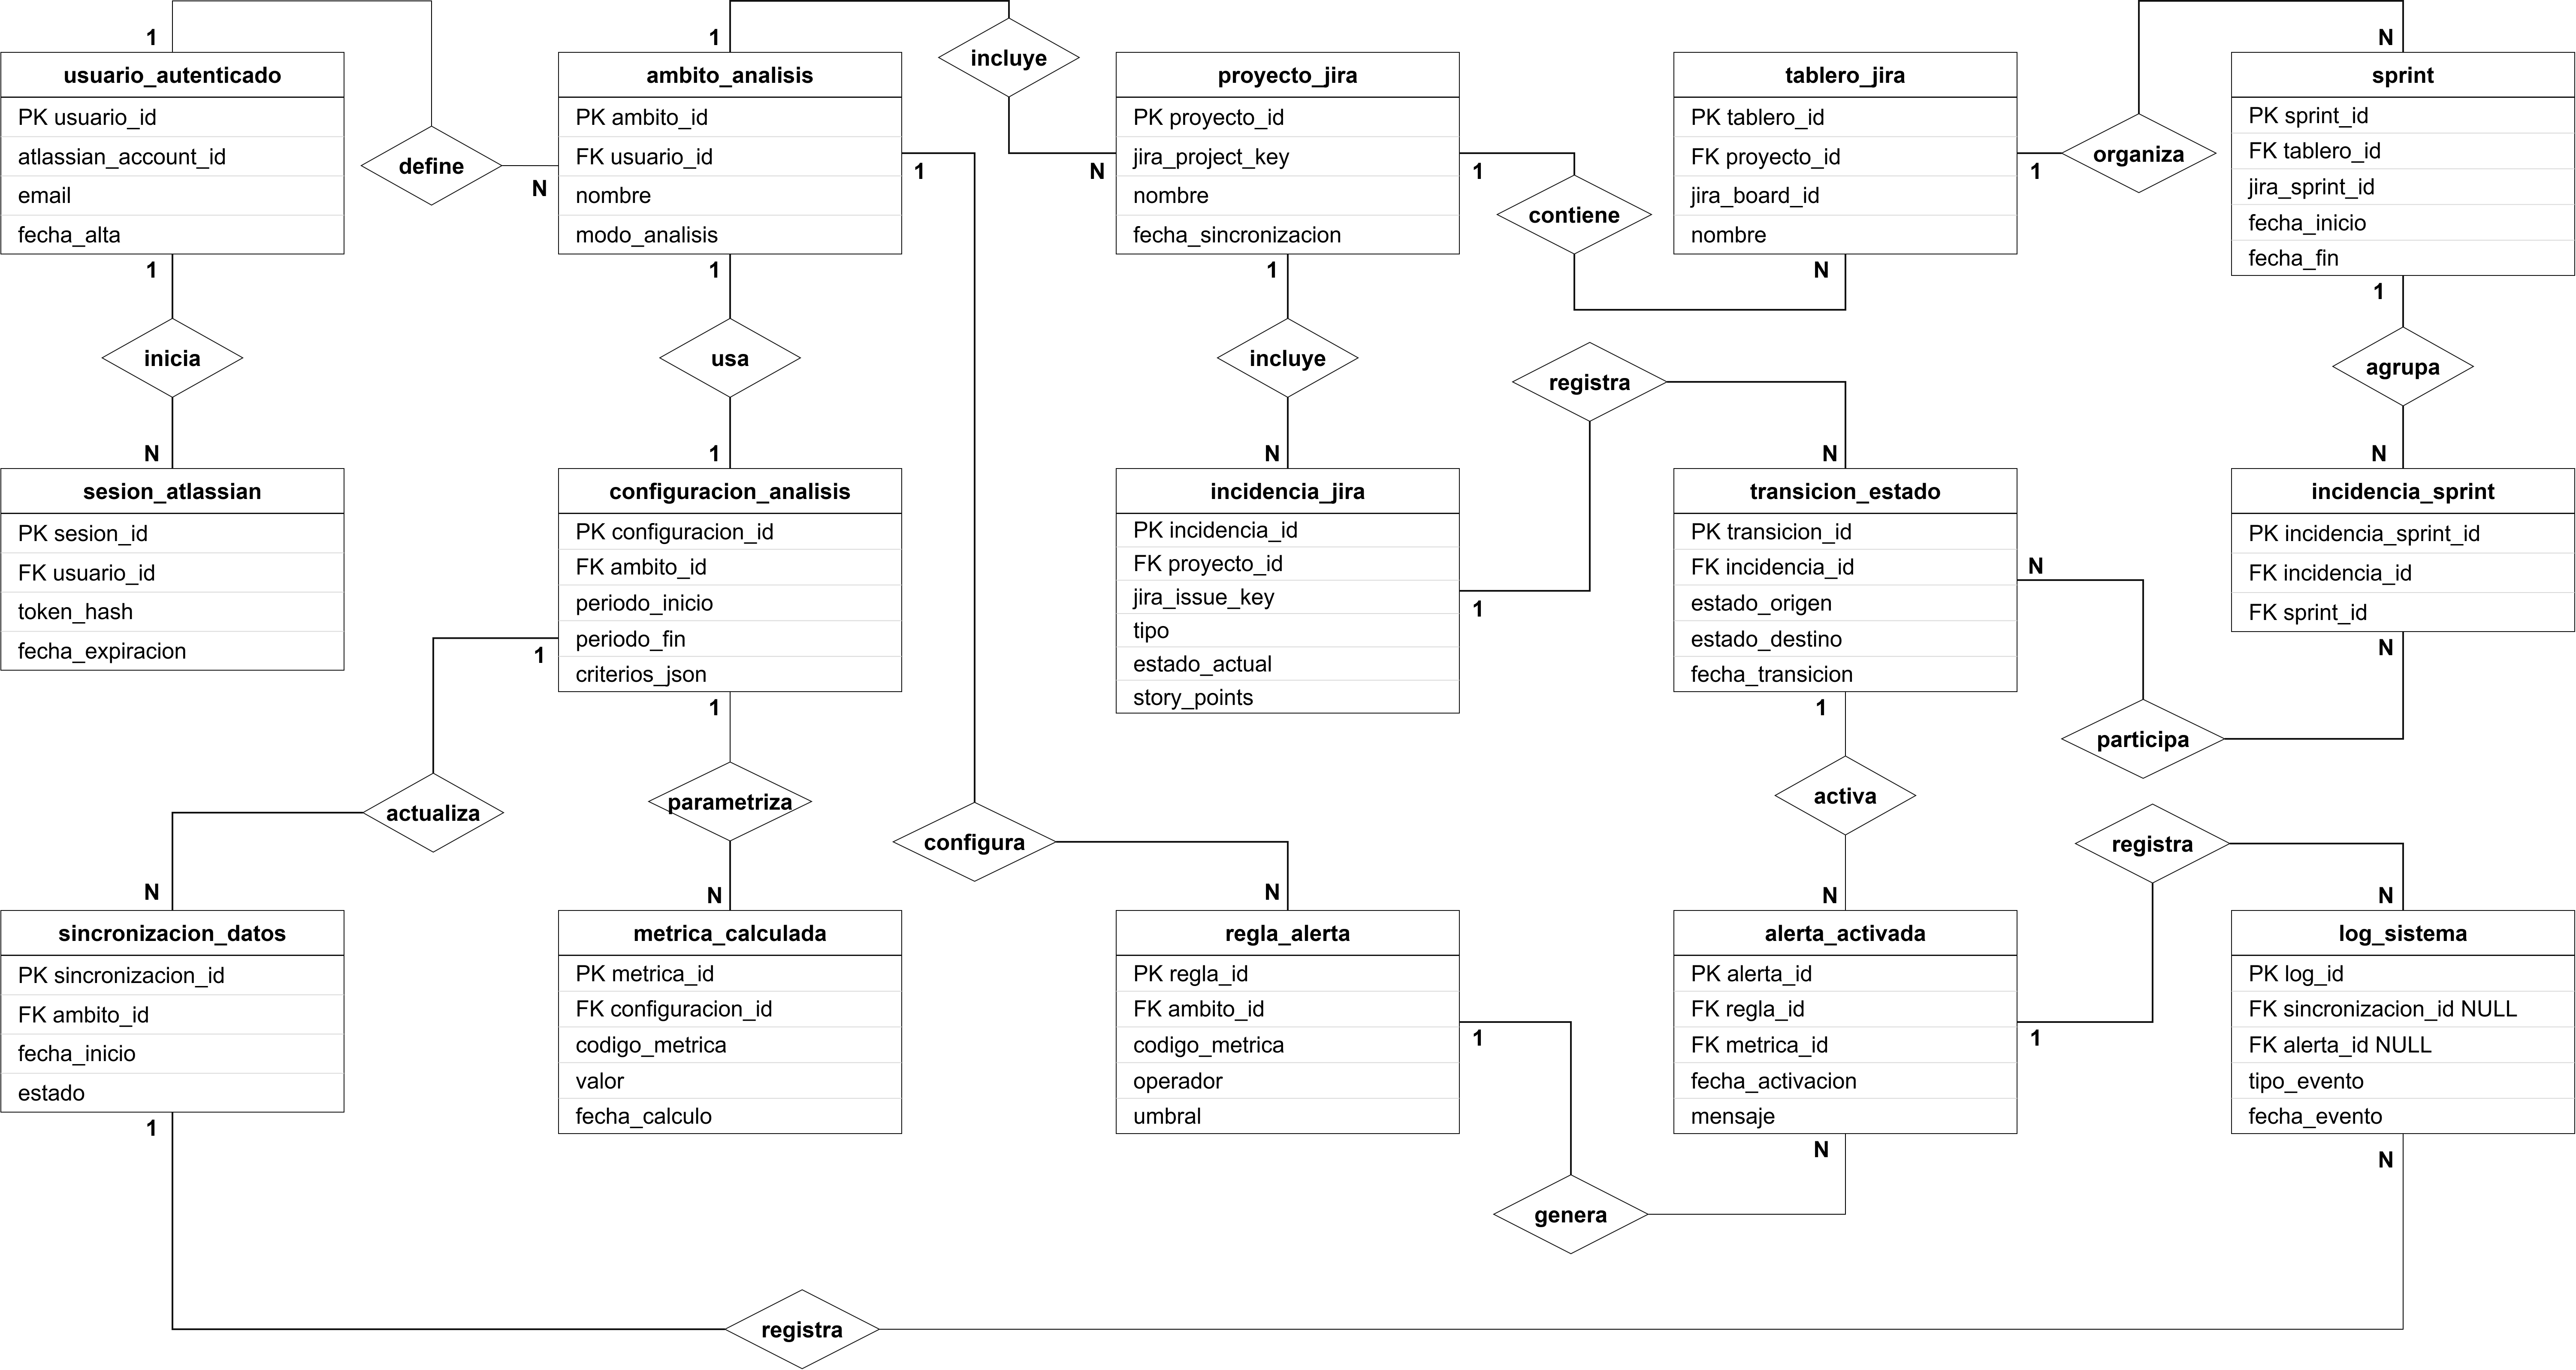
\includegraphics[width=1.25\textwidth]{diagrams/entidad-relacion-base-datos.png}}
    \caption{Diagrama entidad-relación de la base de datos}
    \label{fig:entidad-relacion-base-datos}
\end{figure}

La Figura~\ref{fig:entidad-relacion-base-datos} toma como referencia las entidades principales del diagrama de clases, pero las adapta a un modelo persistente. Las tablas puente \texttt{ambito\_proyecto} e \texttt{incidencia\_sprint} permiten resolver relaciones de muchos a muchos sin duplicar información ni forzar dependencias artificiales.

\begin{itemize}
    \item \texttt{usuario\_autenticado}, \texttt{sesion\_atlassian}, \texttt{ambito\_analisis} y \texttt{configuracion\_analisis}: almacenan la información del usuario, sus sesiones de Atlassian y los criterios de análisis definidos para cada ámbito. Un usuario puede iniciar varias sesiones y definir varios ámbitos; cada ámbito mantiene una configuración de análisis.
    \item \texttt{proyecto\_jira}, \texttt{tablero\_jira}, \texttt{sprint}, \texttt{incidencia\_jira} y \texttt{transicion\_estado}: representan los datos sincronizados desde Jira. Un proyecto puede contener varios tableros e incidencias, un tablero organiza sprints y una incidencia registra sus transiciones de estado para calcular métricas de flujo.
    \item \texttt{ambito\_proyecto} e \texttt{incidencia\_sprint}: actúan como tablas intermedias. La primera asocia ámbitos de análisis con proyectos Jira; la segunda relaciona incidencias con sprints, evitando una relación directa rígida cuando una incidencia pueda aparecer en más de una iteración.
    \item \texttt{sincronizacion\_datos}, \texttt{metrica\_calculada}, \texttt{regla\_alerta}, \texttt{alerta\_activada} y \texttt{log\_sistema}: guardan la actividad interna del sistema. Las sincronizaciones actualizan un ámbito, las métricas se calculan a partir de la configuración vigente, las reglas evalúan dichas métricas y las alertas y logs conservan la trazabilidad del funcionamiento.
\end{itemize}
\clearpage
\section{Diagrama de componentes/arquitectura lógica}

El diagrama de componentes permite representar la organización modular del sistema y las dependencias entre sus partes. Según la especificación oficial de UML de OMG, un componente encapsula una parte sustituible del sistema y expone o requiere interfaces para colaborar con otros elementos~\cite{OMGUML251}. En este trabajo se utiliza esta notación para mostrar una vista lógica de la arquitectura, independiente de decisiones concretas de despliegue.

\begin{figure}[htbp]
    \centering
    \makebox[\textwidth][c]{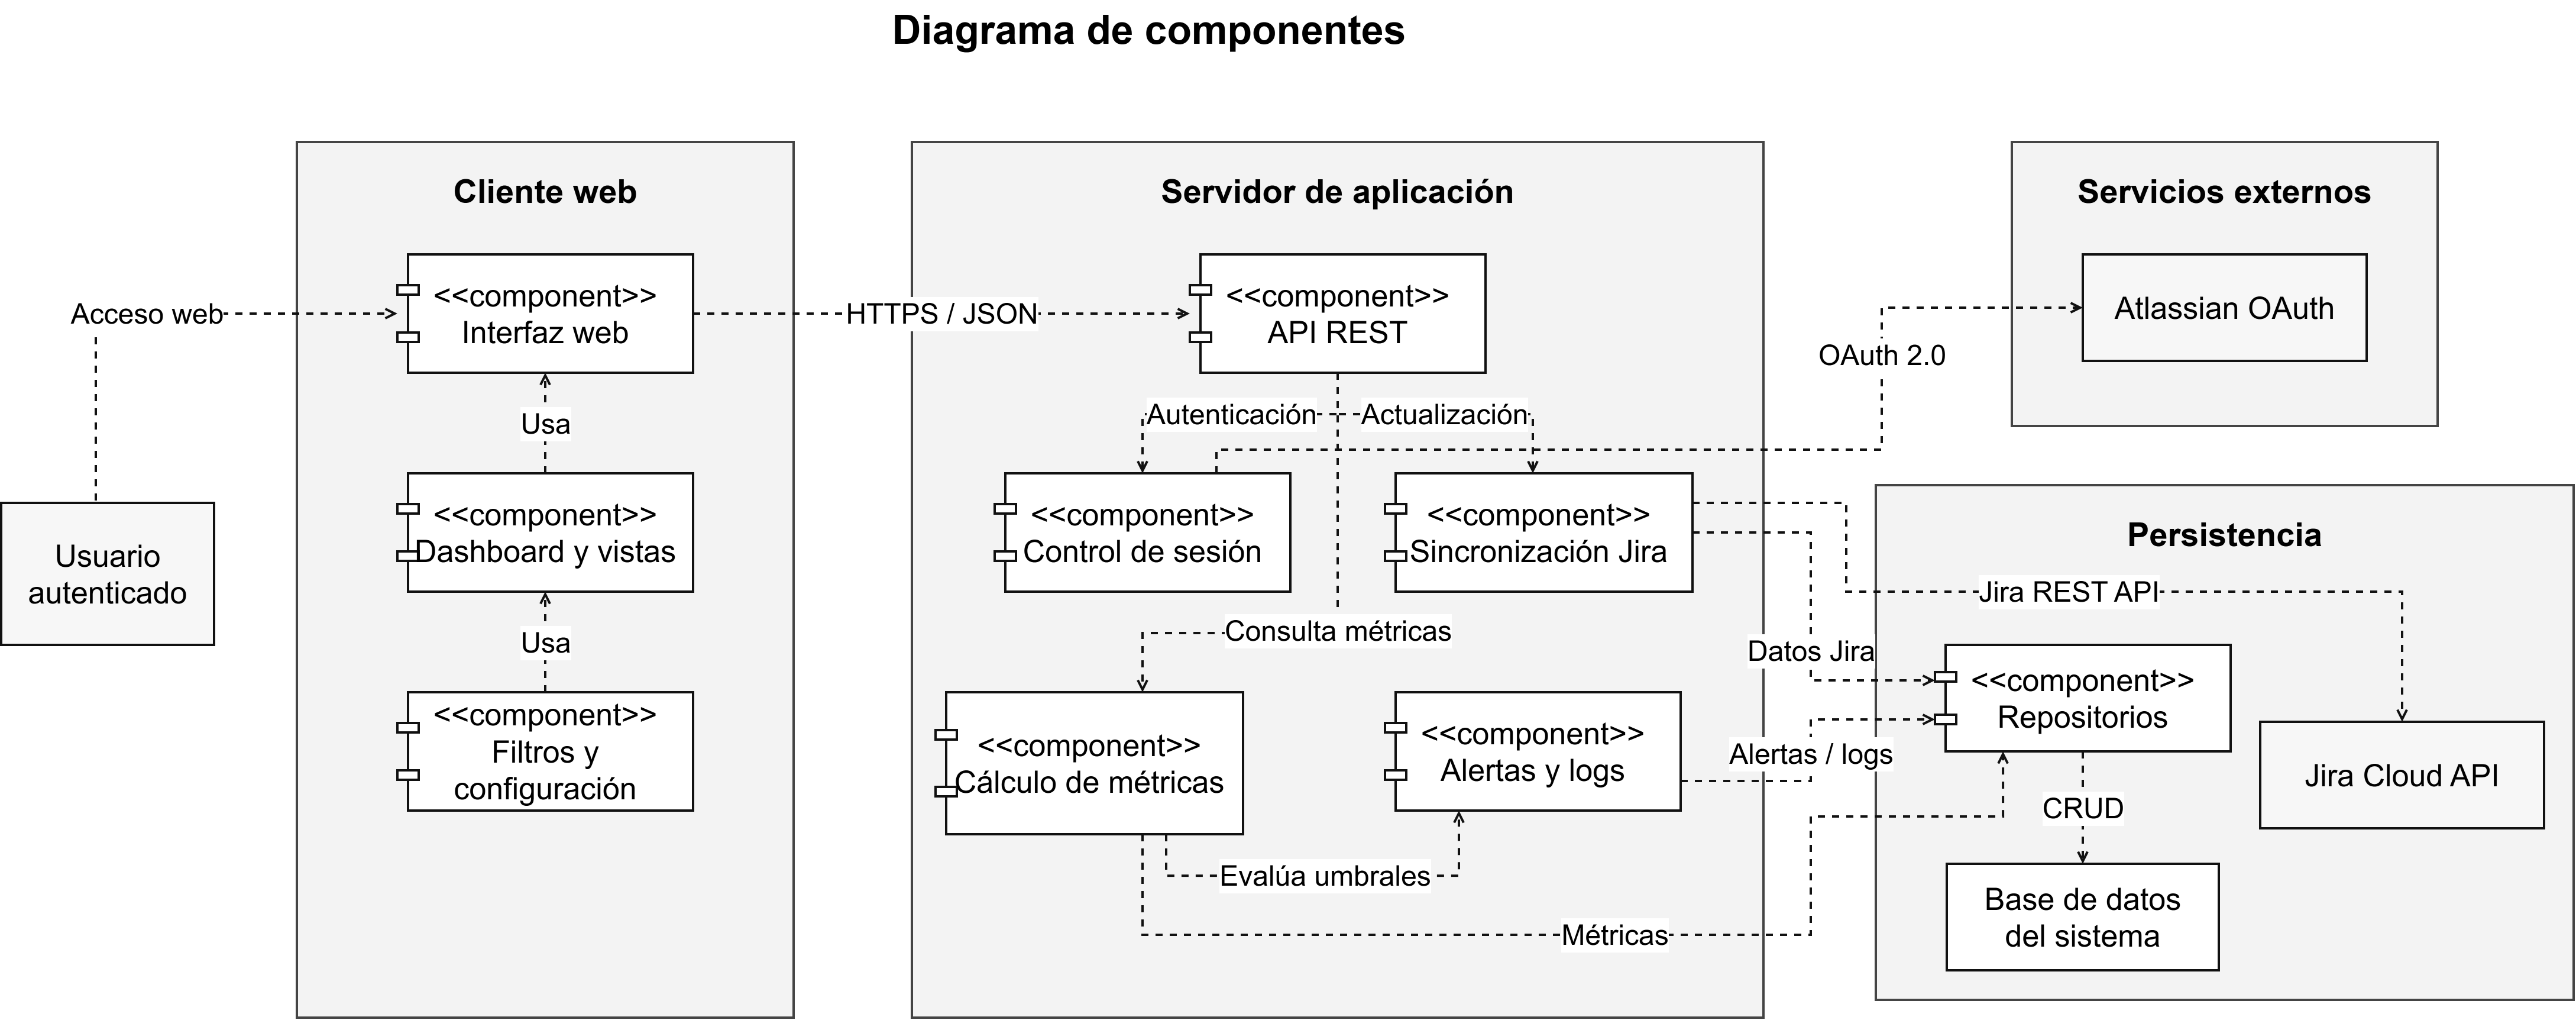
\includegraphics[width=1.25\textwidth]{diagrams/componentes-arquitectura-sistema.png}}
    \caption{Diagrama de componentes y arquitectura lógica del sistema}
    \label{fig:componentes-arquitectura-sistema}
\end{figure}

La Figura~\ref{fig:componentes-arquitectura-sistema} organiza el sistema en cuatro bloques principales: cliente web, servidor de aplicación, servicios externos y persistencia. Las flechas discontinuas representan dependencias entre componentes, es decir, relaciones de uso necesarias para completar las funcionalidades previstas.

\begin{itemize}
    \item \textbf{Cliente web}: agrupa la \texttt{Interfaz web}, el \texttt{Dashboard y vistas} y los componentes de \texttt{Filtros y configuración}. Este bloque permite al usuario autenticado consultar métricas, modificar criterios de análisis y acceder a las vistas principales del sistema.
    \item \textbf{Servidor de aplicación}: contiene la \texttt{API REST}, que centraliza las peticiones del cliente, y los componentes internos encargados del control de sesión, la sincronización con Jira, el cálculo de métricas y la gestión de alertas y logs.
    \item \textbf{Servicios externos}: representan las dependencias con Atlassian. \texttt{Atlassian OAuth} se utiliza para la autenticación del usuario y \texttt{Jira Cloud API} proporciona los datos de proyectos, tableros, sprints e incidencias.
    \item \textbf{Persistencia}: incluye los \texttt{Repositorios}, que aíslan el acceso a datos, y la \texttt{Base de datos del sistema}, donde se almacenan datos sincronizados, configuraciones, métricas calculadas, alertas y logs.
\end{itemize}

Las relaciones principales muestran que el usuario accede al cliente web, el cliente consume la \texttt{API REST} mediante peticiones HTTP y el backend coordina las operaciones internas. El \texttt{Control de sesión} depende de \texttt{Atlassian OAuth}; la \texttt{Sincronización Jira} consulta \texttt{Jira Cloud API}; el \texttt{Cálculo de métricas} trabaja sobre los datos sincronizados; y el componente de \texttt{Alertas y logs} registra eventos y evalúa umbrales a partir de las métricas disponibles. Finalmente, los repositorios concentran la lectura y escritura sobre la base de datos para mantener separada la lógica de negocio del almacenamiento.





\chapter{Análisis del sistema}

Este capítulo recoge los modelos de análisis utilizados para representar la estructura conceptual de Nuvlo y la información que debe persistirse. A diferencia del capítulo de requisitos, que describe qué debe ofrecer el sistema desde el punto de vista funcional, estos diagramas ayudan a razonar sobre el dominio, sus entidades principales y las relaciones entre ellas.

\section{Diagrama de clases}

El diagrama de clases muestra la estructura estática principal del sistema y las relaciones entre los conceptos del dominio. En este caso se representa una vista de análisis previa a la implementación, por lo que las clases describen entidades y responsabilidades del sistema sin depender de una tecnología concreta.

\begin{landscape}
\begin{figure}[p]
    \centering
    \makebox[\linewidth][c]{%
        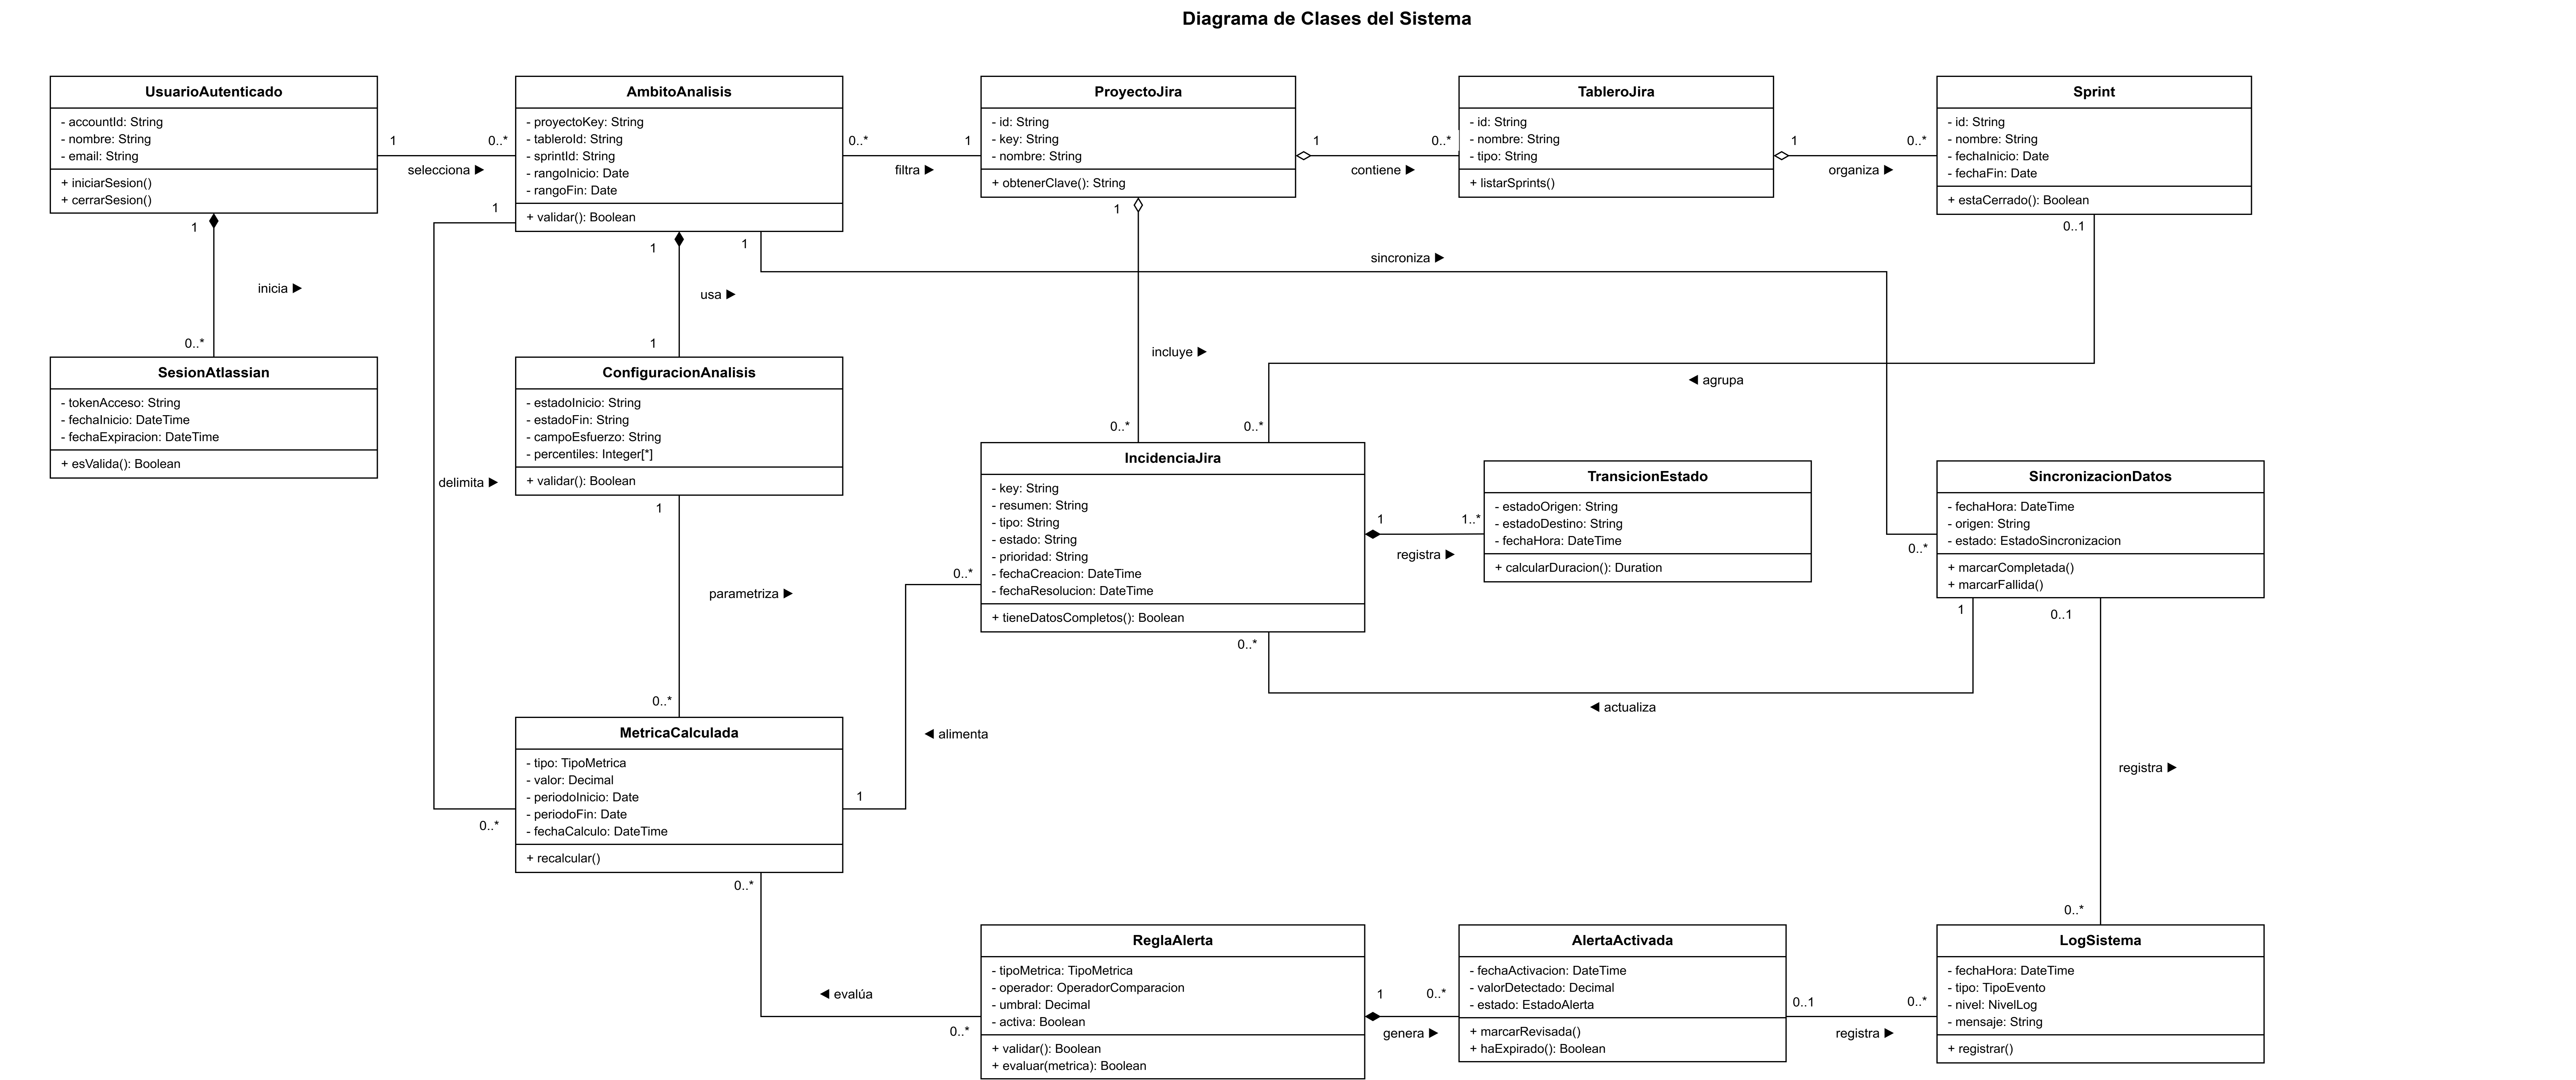
\includegraphics[width=1.12\linewidth,height=0.86\textheight,keepaspectratio]{diagrams/clases-dominio-sistema.png}%
    }
    \caption{Diagrama de clases del sistema}
    \label{fig:clases-dominio-sistema}
\end{figure}
\end{landscape}

La Figura~\ref{fig:clases-dominio-sistema} se interpreta a partir de los verbos situados sobre cada relación. El triángulo del verbo indica la dirección de lectura y las cardinalidades de los extremos concretan cuántas instancias pueden participar en cada asociación. En cuanto a la notación UML, según la especificación oficial de OMG \cite{OMGUML251}, el rombo blanco representa una agregación, es decir, una relación todo-parte débil en la que la parte puede existir de forma independiente. El rombo negro representa una composición, una relación todo-parte fuerte en la que la parte depende del ciclo de vida del todo.

Además de identificar las clases, es necesario indicar qué papel desempeña cada una dentro del dominio. La Tabla~\ref{tab:responsabilidades-clases} resume las responsabilidades principales y los atributos o conceptos más relevantes asociados a cada clase. Estos atributos no pretenden sustituir al diseño físico de la base de datos, sino aclarar qué información mínima necesita manejar el sistema para cumplir los casos de uso definidos.

\begin{landscape}
{\footnotesize
\begin{longtable}{>{\raggedright\arraybackslash}p{5.0cm}>{\raggedright\arraybackslash}p{8.0cm}>{\raggedright\arraybackslash}p{10.2cm}}
\caption{Responsabilidades y atributos principales de las clases del dominio}
\label{tab:responsabilidades-clases}\\
\toprule
\textbf{Clase} & \textbf{Responsabilidad principal} & \textbf{Atributos o información principal} \\
\midrule
\endfirsthead
\toprule
\textbf{Clase} & \textbf{Responsabilidad principal} & \textbf{Atributos o información principal} \\
\midrule
\endhead
\bottomrule
\endfoot
\texttt{UsuarioAutenticado} & Representar al usuario que accede a Nuvlo y delimitar la propiedad de sesiones, ámbitos de análisis y configuraciones. & Identificador interno, identificador de cuenta Atlassian, nombre visible, correo electrónico, fecha de alta, fecha de último acceso y estado de la cuenta. \\
\texttt{SesionAtlassian} & Mantener la información necesaria para operar en nombre del usuario autenticado sin pedir credenciales locales. & Identificador de sesión, usuario asociado, \textit{cloudId}, \textit{scopes} concedidos, fecha de creación, fecha de expiración y referencia segura a los \textit{tokens}. \\
\texttt{AmbitoAnalisis} & Definir el subconjunto de datos sobre el que se calculan métricas y se muestran resultados. & Nombre del ámbito, usuario propietario, proyectos incluidos, tablero o \textit{sprint} seleccionado, rango temporal, filtros activos y fecha de última sincronización. \\
\texttt{ConfiguracionAnalisis} & Recoger los criterios que modifican la interpretación de los datos y el cálculo de métricas. & Estados de inicio y fin, estados considerados trabajo en curso, campo de esfuerzo, percentiles visibles, agrupación temporal y criterios de exclusión. \\
\texttt{ProyectoJira} & Representar un proyecto importado desde Jira y servir como contenedor lógico de tableros e incidencias. & Clave del proyecto, nombre, identificador Jira, URL de origen, tipo de proyecto y fecha de última actualización local. \\
\texttt{TableroJira} & Modelar un tablero de trabajo de Jira asociado a un proyecto y usado para organizar la consulta de \textit{sprints}. & Identificador Jira del tablero, nombre, tipo de tablero, proyecto asociado y fecha de sincronización. \\
\texttt{Sprint} & Representar una iteración temporal utilizada para calcular \textit{Velocity} y analizar evolución por periodos. & Identificador Jira del \textit{sprint}, nombre, estado, fecha de inicio, fecha de fin, fecha de cierre y tablero asociado. \\
\texttt{IncidenciaJira} & Representar cada unidad de trabajo sincronizada desde Jira y aportar los datos base para métricas de flujo. & Clave, resumen, tipo, estado actual, prioridad, estimación, fecha de creación, fecha de resolución, proyecto asociado y responsable si está disponible. \\
\texttt{TransicionEstado} & Registrar los cambios de estado de una incidencia para reconstruir su recorrido y calcular tiempos. & Incidencia asociada, estado origen, estado destino, fecha de transición y origen de la información sincronizada. \\
\texttt{SincronizacionDatos} & Controlar cada proceso de actualización desde Jira o desde el conjunto de datos de demostración. & Ámbito afectado, instante de inicio y fin, estado de ejecución, número de elementos procesados, errores detectados y resumen del resultado. \\
\texttt{MetricaCalculada} & Almacenar el resultado de un cálculo de métrica para un ámbito, periodo y configuración concreta. & Tipo de métrica, valor agregado, periodo, percentiles, número de incidencias consideradas, fecha de cálculo y configuración utilizada. \\
\texttt{ReglaAlerta} & Definir condiciones configurables que permiten avisar al usuario ante valores relevantes de una métrica. & Métrica objetivo, operador, umbral, severidad, estado activo/inactivo, ámbito asociado y fecha de creación. \\
\texttt{AlertaActivada} & Representar una ocurrencia concreta generada cuando una regla cumple su condición. & Regla origen, métrica evaluada, valor observado, severidad, mensaje, fecha de activación y estado de revisión. \\
\texttt{LogSistema} & Conservar eventos relevantes para trazabilidad, depuración y explicación de operaciones internas. & Tipo de evento, severidad, mensaje, usuario o ámbito asociado, fecha de registro, origen del evento y fecha prevista de expiración. \\
\end{longtable}
}
\end{landscape}

A partir de estas responsabilidades se observa una separación entre clases de identidad y configuración, clases procedentes del dominio Jira, clases de cálculo y clases de trazabilidad. Esta división facilita que el sistema pueda sincronizar información externa, conservar una representación local estable y calcular métricas sin depender de una llamada directa a Jira en cada consulta del usuario.

\clearpage
\section{Diagrama entidad-relación de la base de datos}

El diagrama entidad-relación describe la estructura lógica prevista para la persistencia del sistema. A diferencia del diagrama de clases, que representa conceptos del dominio y responsabilidades de análisis, este modelo se centra en tablas, claves primarias, claves foráneas y cardinalidades. Para facilitar su lectura se emplean entidades rectangulares con sus atributos internos y relaciones representadas mediante rombos, siguiendo la forma habitual de los diagramas entidad-relación y las formas disponibles en draw.io para modelos de bases de datos~\cite{DrawioERTables}. Cada rombo contiene un verbo que describe la relación y las cardinalidades se sitúan junto a los extremos conectados. Los nombres de tablas y columnas se han planteado en minúsculas y con \texttt{snake\_case}, siguiendo criterios habituales de estilo SQL~\cite{HolywellSQLStyle}; además, se evitan estructuras innecesariamente complejas para mantener un diseño comprensible y normalizado, de acuerdo con las recomendaciones generales de diseño relacional recogidas por Karwin~\cite{Karwin2010SQLAntipatterns}.

\begin{figure}[htbp]
    \centering
    \makebox[\textwidth][c]{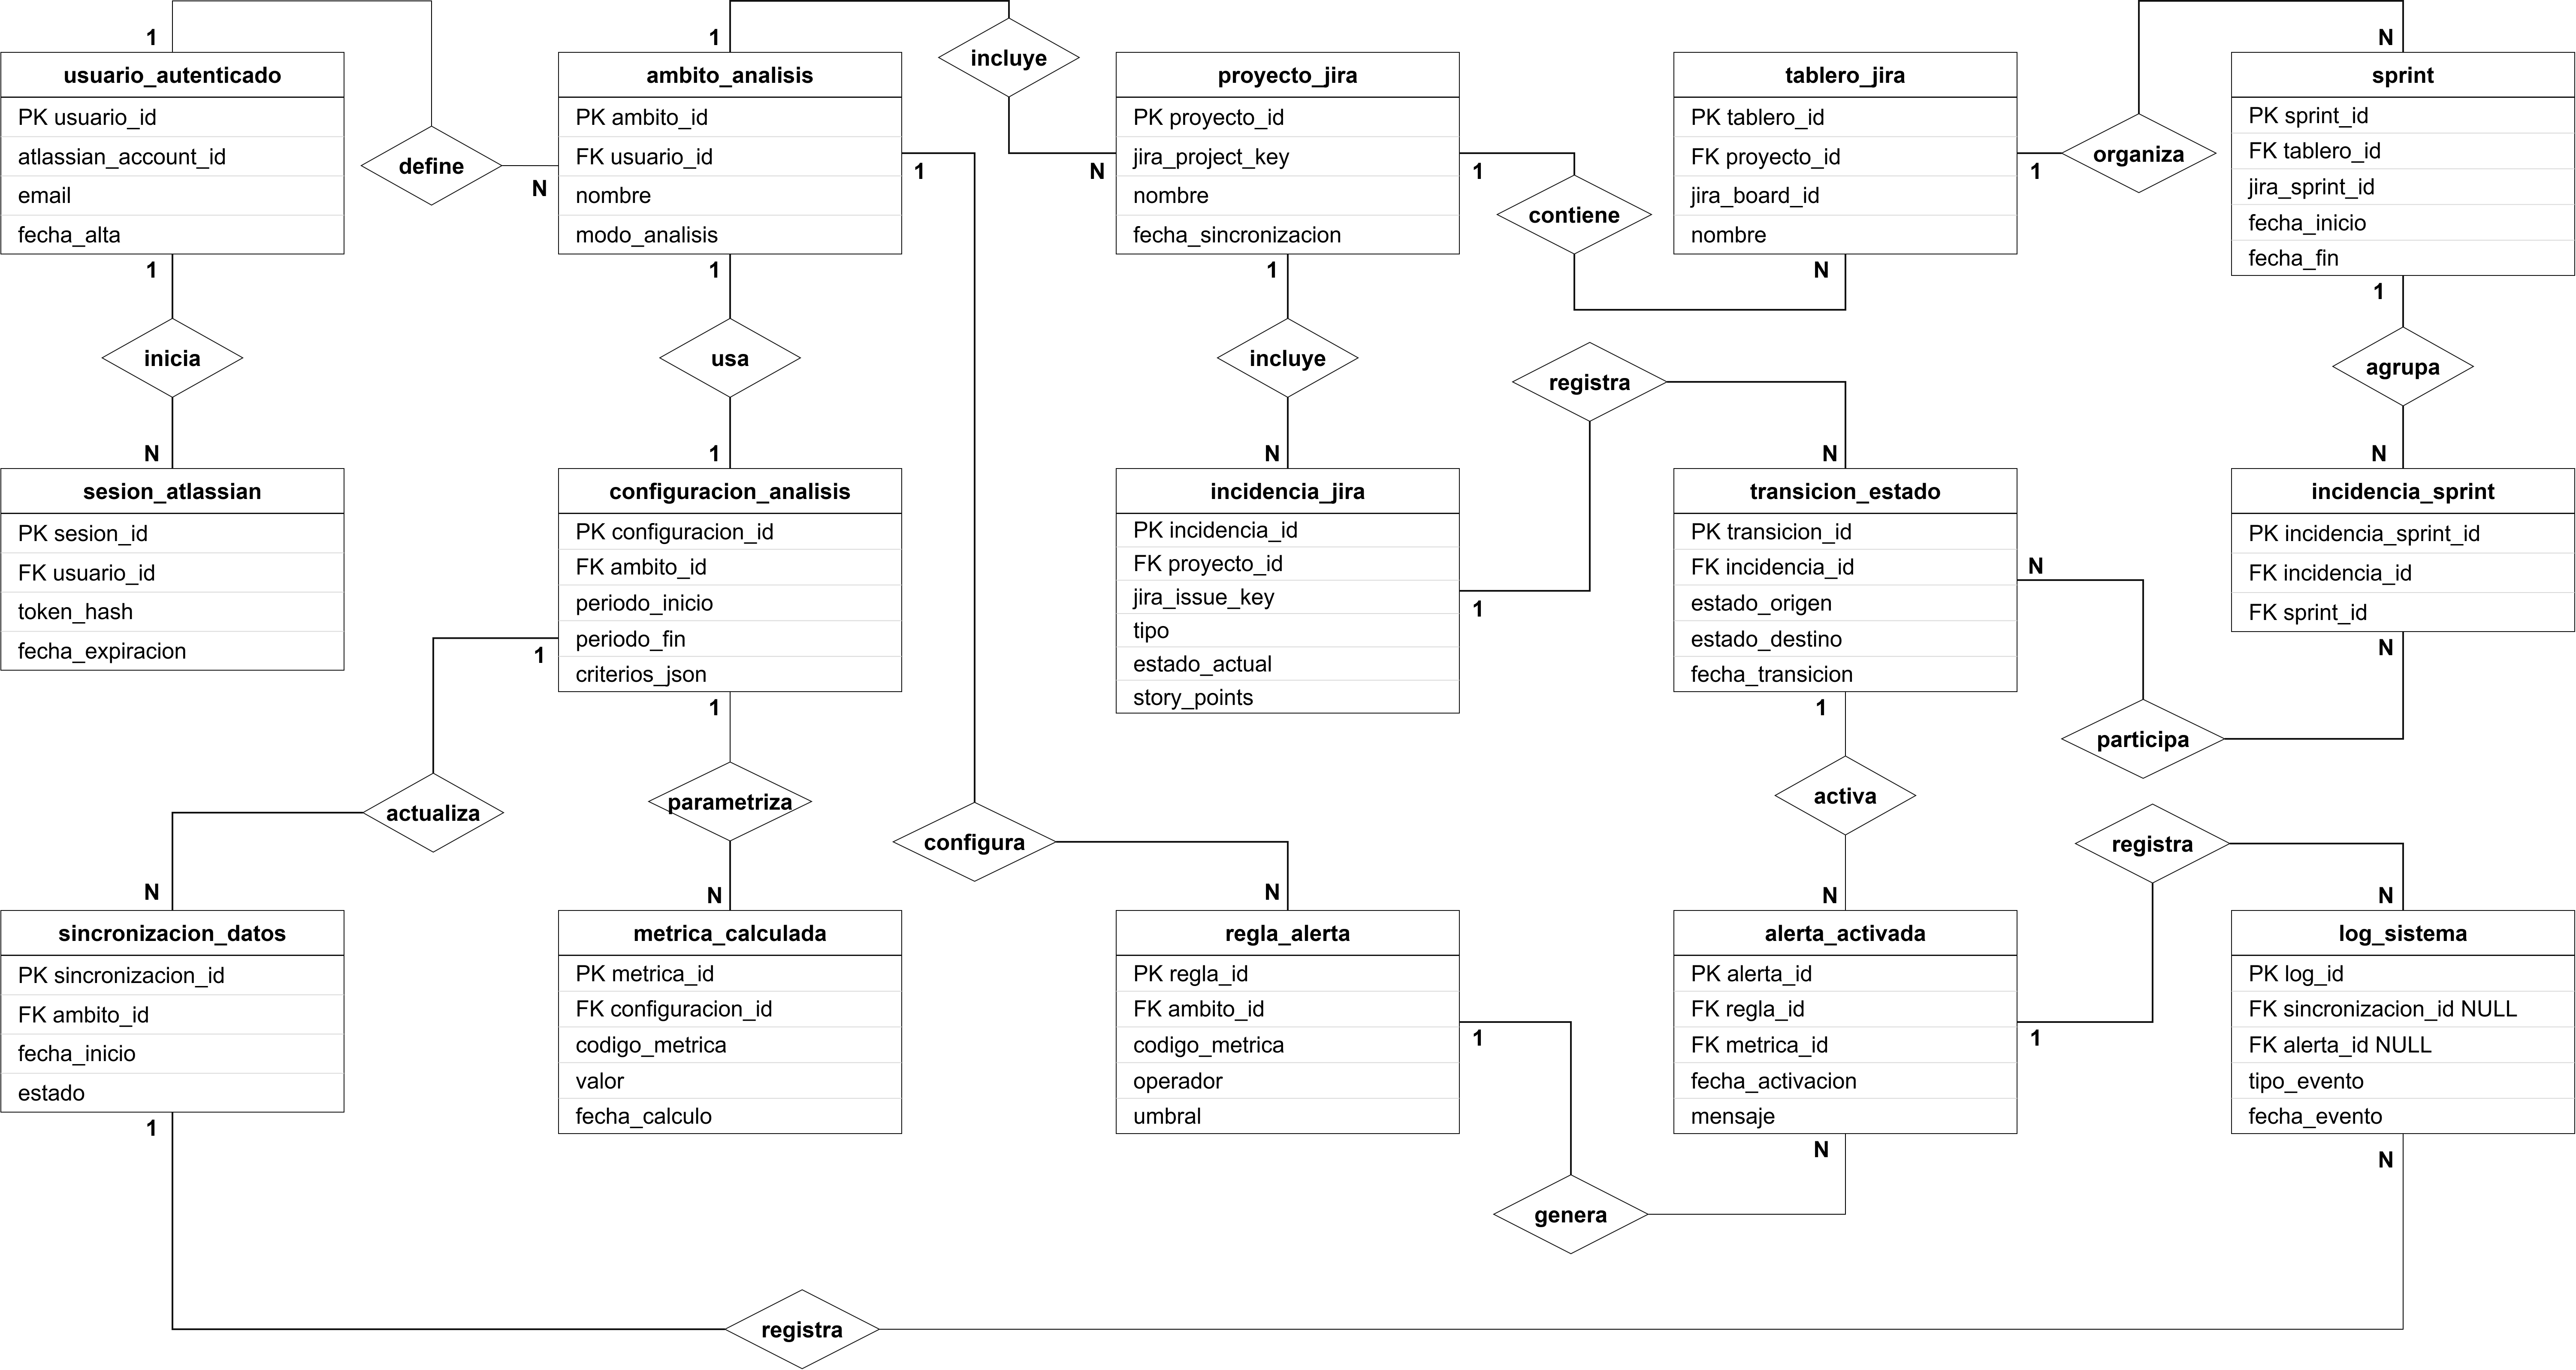
\includegraphics[width=1.25\textwidth]{diagrams/entidad-relacion-base-datos.png}}
    \caption{Diagrama entidad-relación de la base de datos}
    \label{fig:entidad-relacion-base-datos}
\end{figure}

La Figura~\ref{fig:entidad-relacion-base-datos} toma como referencia las entidades principales del diagrama de clases, pero las adapta a un modelo persistente. Las tablas puente \texttt{ambito\_proyecto} e \texttt{incidencia\_sprint} permiten resolver relaciones de muchos a muchos sin duplicar información ni forzar dependencias artificiales.

\begin{itemize}
    \item \texttt{usuario\_autenticado}, \texttt{sesion\_atlassian}, \texttt{ambito\_analisis} y \texttt{configuracion\_analisis}: almacenan la información del usuario, sus sesiones de Atlassian y los criterios de análisis definidos para cada ámbito. Un usuario puede iniciar varias sesiones y definir varios ámbitos; cada ámbito mantiene una configuración de análisis.
    \item \texttt{proyecto\_jira}, \texttt{tablero\_jira}, \texttt{sprint}, \texttt{incidencia\_jira} y \texttt{transicion\_estado}: representan los datos sincronizados desde Jira. Un proyecto puede contener varios tableros e incidencias, un tablero organiza \textit{sprints} y una incidencia registra sus transiciones de estado para calcular métricas de flujo.
    \item \texttt{ambito\_proyecto} e \texttt{incidencia\_sprint}: actúan como tablas intermedias. La primera asocia ámbitos de análisis con proyectos Jira; la segunda relaciona incidencias con \textit{sprints}, evitando una relación directa rígida cuando una incidencia pueda aparecer en más de una iteración.
    \item \texttt{sincronizacion\_datos}, \texttt{metrica\_calculada}, \texttt{regla\_alerta}, \texttt{alerta\_activada} y \texttt{log\_sistema}: guardan la actividad interna del sistema. Las sincronizaciones actualizan un ámbito, las métricas se calculan a partir de la configuración vigente, las reglas evalúan dichas métricas y las alertas y \textit{logs} conservan la trazabilidad del funcionamiento.
\end{itemize}
\clearpage

\chapter{Diseño y arquitectura del sistema}

\section{Enfoque general}

Nuvlo se ha diseñado como una aplicación web de apoyo al análisis de equipos ágiles que trabajan con Jira Cloud. La decisión principal de arquitectura ha sido separar claramente la interfaz, la API, la persistencia y los servicios de integración, manteniendo todo dentro de un monorepo sencillo gestionado con \textit{npm workspaces}~\cite{NpmWorkspaces}. Esta organización permite que frontend, backend, esquema de base de datos, documentación y pruebas evolucionen en el mismo repositorio, lo que facilita la trazabilidad del desarrollo y la revisión del proyecto.

Se descartó dividir el sistema en varios repositorios porque habría aumentado el coste de configuración y coordinación para un proyecto individual. También se evitó mezclar frontend y backend en un único directorio sin separación interna, ya que habría dificultado explicar las responsabilidades de cada parte y mantener una estructura limpia durante la implementación.

\section{Arquitectura lógica}

La arquitectura sigue un esquema cliente-servidor. La aplicación web se ejecuta en el navegador y se comunica con una API propia. La API es la única parte del sistema que interactúa con Jira Cloud, PostgreSQL y Redis. De este modo, el frontend no necesita conocer credenciales ni detalles internos de sincronización.

El frontend se ha implementado con React y Vite~\cite{ReactDocs,ViteDocs}. La API se ha construido con Node.js y Express~\cite{NodeDocs,ExpressDocs}. La persistencia principal se realiza con PostgreSQL, accedida mediante Prisma~\cite{PostgreSQLDocs,PrismaDocs}. Redis se utiliza como almacenamiento temporal para datos de sesión, estados de seguridad del flujo OAuth y elementos de corta duración~\cite{RedisDocs}. El entorno local se levanta mediante Docker Compose~\cite{DockerComposeDocs}.

Los diagramas incluidos en la memoria representan esta separación por capas y ayudan a entender el recorrido de los datos: el usuario entra por la interfaz, la API valida la sesión, sincroniza información desde Jira cuando procede y consulta la base de datos local para construir las métricas visibles en el dashboard.

\section{Modelo de datos y sincronización}

El modelo de datos se orienta a conservar una copia local de la información necesaria para calcular métricas ágiles. Se almacenan proyectos, incidencias, sprints, estados y datos de transición cuando están disponibles. Esta decisión evita que cada interacción de la interfaz dependa de una llamada directa a Jira Cloud y permite recalcular métricas de forma controlada.

La sincronización se realiza por ámbitos concretos, no como una descarga completa indiscriminada. El sistema solicita únicamente los campos necesarios y trabaja con paginación de la API de Jira~\cite{AtlassianJiraRestV3,AtlassianJiraIssuesApi}. Esta aproximación reduce el número de llamadas externas y encaja mejor con las restricciones de uso de una API remota.

\section{Seguridad}

El acceso final a Nuvlo se basa en OAuth 2.0 de Atlassian, concretamente en el flujo 3LO~\cite{AtlassianOAuth3LO}. El usuario no crea una cuenta local con contraseña: autoriza la aplicación con su cuenta de Atlassian y Nuvlo crea o actualiza la sesión asociada a ese usuario.

Para proteger el proceso de autenticación se han incorporado medidas habituales en aplicaciones web modernas: parámetro \textit{state}, PKCE y protección CSRF~\cite{OWASPOAuth2,OWASPCSRF}. Los tokens no se exponen al navegador como credenciales persistentes de larga duración. La API actúa como capa intermedia y aplica validaciones antes de permitir operaciones protegidas.

\section{Diseño de interfaz}

El diseño visual parte de los prototipos realizados durante la fase de análisis y de los diagramas de vistas incluidos en la memoria. La interfaz final no replica cada prototipo de forma literal, pero conserva su planteamiento: navegación lateral, dashboard principal, vista de tablero, alertas, actividad y configuración.

La estética de Nuvlo se apoya en una identidad propia basada en la idea de ``nube + flujo''. Para el dashboard se tomó como inspiración visual una plantilla pública de administración moderna de Morphin~\cite{MorphinDashboardInspiration}, sin reutilizar su código fuente. La referencia se usó únicamente para orientar decisiones de composición, tarjetas, jerarquía visual y navegación.

\section{Relación con los anexos}

Los capítulos principales explican las decisiones de diseño y el resultado técnico. Los anexos cumplen una función complementaria: el manual de usuario muestra cómo utilizar la aplicación, el manual de código fuente resume la organización del repositorio y los comandos principales, y el anexo de uso de IA documenta el apoyo recibido durante el desarrollo. Por tanto, puede existir cierta relación temática entre capítulos y anexos, pero no se considera redundante si cada parte mantiene un nivel de detalle distinto.

\chapter{Implementación}

\section{Stack tecnológico}

La implementación de Nuvlo se ha realizado con un stack JavaScript/Node orientado a desarrollo web moderno. En el cliente se usa React para construir la interfaz y Vite como herramienta de desarrollo y empaquetado~\cite{ReactDocs,ViteDocs}. En el servidor se usa Node.js con Express para exponer la API HTTP~\cite{NodeDocs,ExpressDocs}. La capa de datos se apoya en Prisma como ORM y PostgreSQL como base de datos relacional~\cite{PrismaDocs,PostgreSQLDocs}.

Redis se incorpora como servicio auxiliar para datos efímeros y operaciones de apoyo, mientras que Docker Compose facilita reproducir el entorno local con los servicios necesarios~\cite{RedisDocs,DockerComposeDocs}. Esta combinación permite mantener una separación clara entre la lógica de negocio, la interfaz y la infraestructura de desarrollo.

\section{Frontend}

El \textit{frontend} organiza la experiencia alrededor de varias vistas principales: entrada con Jira, \textit{dashboard}, tablero, alertas, actividad y configuración. El \textit{dashboard} muestra las métricas principales, gráficos y \textit{widgets} configurables. La navegación se ha ajustado para mantener coherencia con los prototipos de la memoria y para funcionar tanto en escritorio como en móvil.

Se han añadido transiciones visuales ligeras para que los cambios de vista, paneles y acciones clicables no produzcan una sensación de parpadeo. Estas animaciones son sencillas y no introducen dependencias pesadas, por lo que no afectan de forma significativa al rendimiento de la aplicación.

\section{Backend e integración con Jira}

El \textit{backend} encapsula la comunicación con Jira Cloud. Cuando el usuario inicia sesión, la aplicación redirige a Atlassian y recibe el resultado del flujo OAuth. A partir de esa sesión, el servidor puede consultar los recursos autorizados de Jira y sincronizar la información necesaria para calcular las métricas.

La integración no calcula las métricas consultando Jira en cada carga del \textit{dashboard}. En su lugar, sincroniza los datos relevantes, los persiste en PostgreSQL y después la aplicación consulta su propia base de datos. Esto mejora la estabilidad de la interfaz, reduce dependencia de la red y facilita auditar qué datos se usaron para obtener cada resultado.

\section{Métricas implementadas}

El sistema calcula \textit{WIP}, \textit{Velocity}, \textit{Lead Time} y \textit{Cycle Time}. \textit{WIP} representa el trabajo en curso según el estado de las incidencias visibles. \textit{Velocity} resume el trabajo completado por periodo o \textit{sprint}. \textit{Lead Time} y \textit{Cycle Time} se calculan a partir de fechas de creación, resolución y transiciones cuando la información está disponible.

En Jira real, la calidad de estas métricas depende de cómo se haya usado el tablero y de si existen transiciones suficientes en el historial. Por este motivo, el proyecto incluye también una demo \textit{offline} con datos controlados, útil para validar escenarios que en una instancia real recién creada pueden no tener todavía histórico suficiente.

\section{Alertas, actividad y retención de datos}

La fase de interfaz incluye reglas de alerta basadas en umbrales, notificaciones visuales y un registro de actividad. Las alertas permiten avisar al usuario cuando una métrica supera una condición definida. El registro de actividad guarda eventos de uso relevantes, como sincronizaciones, cambios de sesión, creación de reglas, activación de alertas y tareas de limpieza.

La política de retención diferencia entre datos persistentes, datos operativos y datos efímeros. PostgreSQL conserva la información necesaria para análisis e histórico: proyectos importados, incidencias, transiciones, métricas calculadas, reglas de alerta y sincronizaciones. Estos datos son los que permiten reconstruir el estado mostrado en el \textit{dashboard} y justificar los resultados obtenidos.

Redis se reserva para información temporal: estados del flujo OAuth, valores CSRF, verificadores PKCE, cachés de corta duración y datos auxiliares que no deben mantenerse indefinidamente. Estos elementos se almacenan con tiempo de vida limitado mediante TTL, de forma que expiran automáticamente sin requerir limpieza manual~\cite{RedisDocs}.

Para evitar crecimiento indefinido de la base de datos, los \textit{logs} de actividad y el historial de alertas se tratan como datos retenibles. La aplicación contempla tareas de limpieza que eliminan o archivan registros antiguos según una ventana configurable. De este modo, se mantiene la trazabilidad necesaria para depuración y auditoría básica sin convertir PostgreSQL en un almacén ilimitado de eventos.

\section{Diagrama de despliegue}

El diagrama de despliegue representa la distribución física prevista del sistema sobre nodos de ejecución. Según la notación UML, un nodo modela un recurso computacional o entorno de ejecución, un artefacto representa una unidad desplegable del sistema y las rutas de comunicación indican cómo se conectan dichos nodos durante la ejecución~\cite{OMGUML251}. En este trabajo se utiliza para mostrar cómo se ubican el cliente web, el \textit{backend}, la base de datos, la caché y los servicios externos de Atlassian.

\begin{figure}[htbp]
    \centering
    \makebox[\textwidth][c]{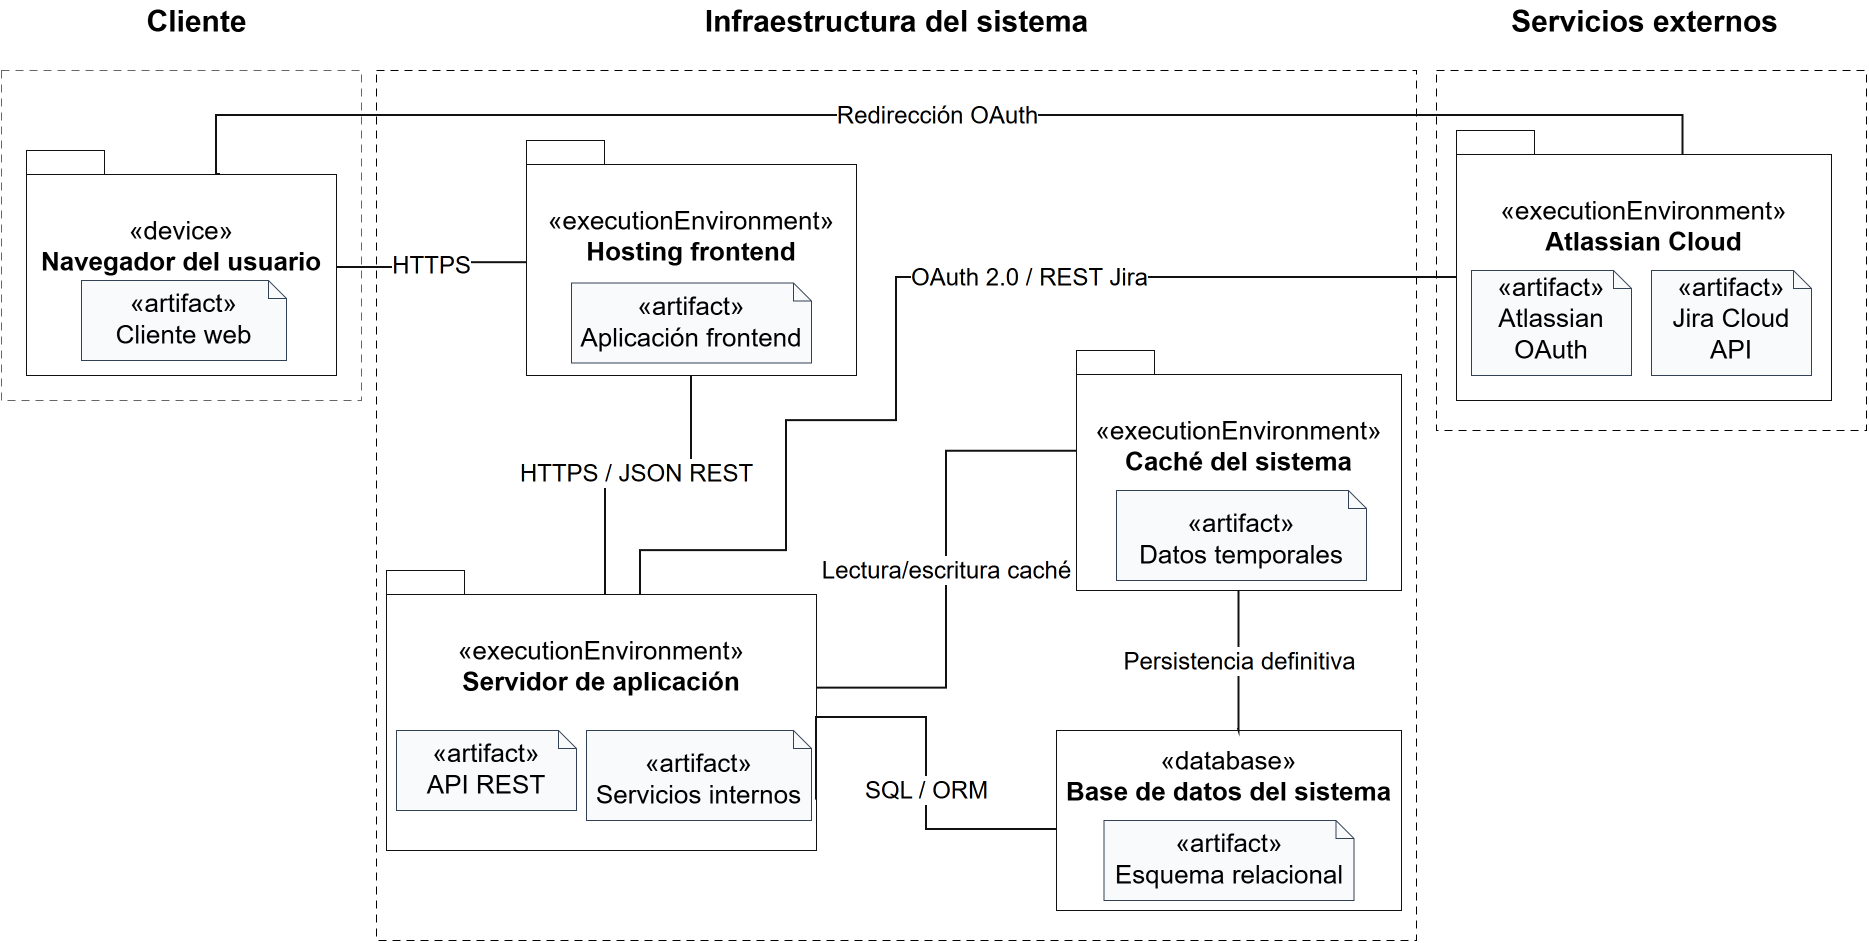
\includegraphics[width=1.25\textwidth]{diagrams/despliegue-sistema.png}}
    \caption{Diagrama de despliegue del sistema}
    \label{fig:despliegue-sistema}
\end{figure}

La Figura~\ref{fig:despliegue-sistema} distingue entre el cliente del usuario, la infraestructura propia del sistema y las dependencias externas. El usuario accede desde su navegador al \textit{frontend} mediante \texttt{HTTPS}; el \textit{frontend} consume la \texttt{API REST} del servidor de aplicación; y el \textit{backend} coordina la autenticación, sincronización, cálculo de métricas, gestión de alertas y acceso a datos.

\begin{itemize}
    \item \textbf{Navegador del usuario}: ejecuta el cliente web y muestra las vistas de panel, tablero, registro, alertas y configuración.
    \item \textbf{Servidor web / hosting \textit{frontend}}: aloja el artefacto \textit{frontend} compuesto por los recursos \texttt{HTML}, \texttt{CSS} y \texttt{JavaScript} de la aplicación.
    \item \textbf{Servidor de aplicación}: despliega la \texttt{API REST} y los servicios internos encargados de sesión, sincronización con Jira, cálculo de métricas y alertas.
    \item \textbf{Caché del sistema}: almacena temporalmente datos recientes de Jira, resultados de métricas o información de sesión para reducir lecturas repetidas y evitar recálculos innecesarios.
    \item \textbf{Base de datos del sistema}: conserva la información persistente, incluyendo datos sincronizados, configuraciones, métricas calculadas, alertas y \textit{logs}.
    \item \textbf{Atlassian Cloud}: agrupa los servicios externos usados por el sistema. \texttt{Atlassian OAuth} permite autenticar al usuario y \texttt{Jira Cloud API} proporciona los datos de proyectos, tableros, \textit{sprints} e incidencias.
\end{itemize}

Las rutas de comunicación muestran que el navegador puede ser redirigido a Atlassian durante la autenticación OAuth, mientras que el servidor de aplicación se comunica con Jira mediante peticiones \texttt{REST}. La caché se sitúa entre la lógica de aplicación y la persistencia para acelerar consultas frecuentes, pero la base de datos mantiene la información definitiva del sistema.
\clearpage

\chapter{Validación y resultados}

\section{Estrategia de validación}

La validación de Nuvlo combina pruebas automatizadas, revisión manual de la interfaz y comprobación con datos reales de Jira. Esta estrategia busca cubrir dos aspectos distintos: que los cálculos internos sean correctos y que la aplicación sea usable en los flujos principales.

Para conectar implementación y requisitos se utiliza una matriz requisito-prueba. En ella, cada requisito funcional, no funcional o de integración se asocia con una prueba, una revisión manual o una evidencia de uso. La matriz completa se recoge en la Tabla~\ref{tab:matriz-requisito-prueba}, dentro del capítulo de requisitos, y se resume en este capítulo desde el punto de vista de la validación.

\section{Tipos de prueba utilizados}

Antes de interpretar la matriz requisito-prueba conviene distinguir los tipos de comprobación empleados durante el desarrollo:

\begin{itemize}
    \item \textbf{Pruebas unitarias}: verifican funciones aisladas, especialmente cálculos de métricas, percentiles, validaciones de datos y reglas de alerta. Se ejecutan con Vitest~\cite{VitestGuide}.
    \item \textbf{Pruebas de integración}: comprueban que varias piezas funcionan juntas, por ejemplo API, repositorios, PostgreSQL, Redis y servicios de sincronización.
    \item \textbf{Pruebas con Jira real}: validan el flujo OAuth, la lectura de proyectos, la sincronización de incidencias y el almacenamiento local de datos procedentes de Jira Cloud.
    \item \textbf{Pruebas con dataset offline}: usan datos controlados para comprobar cálculos que requieren histórico suficiente, como Lead Time, Cycle Time, percentiles o Velocity.
    \item \textbf{Pruebas end-to-end}: recorren la aplicación desde el navegador, incluyendo navegación, filtros, widgets, alertas, logs y modo demo. Se plantean con Playwright~\cite{PlaywrightDocs}.
    \item \textbf{Revisión visual y responsive}: comprueba capturas en escritorio y móvil para validar legibilidad, navegación y coherencia con las vistas previstas.
\end{itemize}

\section{Pruebas automatizadas}

Las pruebas unitarias se centran en cálculos de métricas, percentiles, validaciones y reglas de alerta. Para ello se utiliza Vitest~\cite{VitestGuide}. Las pruebas de integración comprueban el comportamiento de la API, la persistencia y los servicios que dependen de PostgreSQL o Redis. En los casos relacionados con Jira se utilizan datos controlados o respuestas simuladas para evitar depender siempre de una conexión externa.

Las pruebas end-to-end se plantean con Playwright~\cite{PlaywrightDocs}. Su objetivo es recorrer los flujos principales desde el punto de vista del usuario: entrada en modo demo, navegación por vistas, uso de filtros, sincronización, consulta de alertas y revisión del registro de actividad.

\section{Matriz requisito-prueba}

La matriz completa de validación se muestra en la Tabla~\ref{tab:matriz-requisito-prueba}. Para evitar repetir en este capítulo toda la tabla, la Tabla~\ref{tab:resumen-validacion-requisitos} resume la lectura global de esa matriz.

{\renewcommand{\arraystretch}{1.22}\footnotesize
\begin{longtable}{p{3.0cm}p{3.1cm}p{6.0cm}}
\caption{Resumen de la matriz requisito-prueba}\label{tab:resumen-validacion-requisitos}\\
\toprule
\textbf{Bloque} & \textbf{Estado general} & \textbf{Evidencia principal} \\
\midrule
\endfirsthead
\toprule
\textbf{Bloque} & \textbf{Estado general} & \textbf{Evidencia principal} \\
\midrule
\endhead
Integración Jira y autenticación & Cumplido & Flujo OAuth 2.0 3LO, sesión protegida, sincronización de proyecto real y persistencia en PostgreSQL. \\
Dashboard y visualización & Cumplido & Dashboard responsive, filtros rápidos, widgets configurables, ayudas contextuales y capturas de escritorio/móvil. \\
Métricas principales & Cumplido & Cálculo de WIP, Velocity, Lead Time, Cycle Time, media y percentiles con dataset offline y datos sincronizados. \\
Alertas y actividad & Cumplido & Reglas de umbral, contador visual de alertas, notificación emergente, historial de alertas y registro de actividad. \\
Retención, seguridad y mantenimiento & Cumplido & Cookies \texttt{httpOnly}, CSRF, PKCE, cifrado de tokens, Redis con TTL y limpieza de logs/alertas antiguos. \\
Configuración avanzada y métricas futuras & Parcial/Futuro & Configuración básica disponible; quedan como ampliación la configuración avanzada completa, Deployment Frequency y más métricas de flujo. \\
\bottomrule
\end{longtable}
\vspace{0.45em}
}


\section{Validación con Jira real}

La aplicación se ha probado con un proyecto real de Jira creado para demostración. Este escenario permite validar el flujo OAuth, la obtención de proyectos accesibles, la sincronización de incidencias y la persistencia en la base de datos local. Las capturas del manual de usuario muestran la aplicación funcionando con datos procedentes de Jira.

La validación con Jira real también sirve para detectar limitaciones prácticas. Por ejemplo, si las incidencias se crean y cierran en un intervalo muy corto, Lead Time y Cycle Time pueden aparecer como cero o valores poco representativos. Esto no implica que el cálculo esté ausente, sino que el histórico disponible no contiene todavía información temporal suficiente para un análisis realista.

\section{Validación con demo offline}

La demo offline cubre el caso contrario: proporciona datos preparados para que todas las métricas tengan valores visibles y coherentes. Este modo es útil para presentaciones, pruebas sin conexión y comprobaciones de regresión visual. Al no depender de la API de Jira, permite demostrar el comportamiento esperado de la interfaz incluso si la autenticación externa falla o no hay red disponible.

\section{Resultados obtenidos}

El resultado actual es un MVP funcional de Nuvlo. La aplicación permite iniciar sesión con Atlassian, sincronizar información de Jira, consultar métricas ágiles, aplicar filtros, configurar widgets, crear alertas y revisar actividad. Además, dispone de una demo offline que actúa como respaldo para validación y presentación.

El sistema todavía no pretende cubrir todos los escenarios de una herramienta comercial. Algunas mejoras, como métricas avanzadas, despliegue productivo, integración con repositorios de código o análisis predictivo, quedan fuera del alcance principal y se recogen como líneas de trabajo futuro.

\chapter{Conclusiones y trabajo futuro}

\section{Conclusiones}

El desarrollo de Nuvlo ha permitido construir una aplicación web completa para visualizar métricas ágiles a partir de datos de Jira Cloud. El proyecto cubre desde la autenticación con Atlassian hasta la sincronización, persistencia, cálculo de indicadores y presentación en una interfaz \textit{responsive}.

Una de las decisiones más importantes ha sido no depender de Jira en cada interacción de la interfaz. La sincronización hacia una base de datos local mejora la estabilidad, facilita depurar resultados y permite explicar con claridad cómo se calculan las métricas. Esta decisión también encaja con las restricciones habituales de trabajar con APIs externas. Además, la política de retención separa los datos históricos necesarios para el análisis de los datos temporales y \textit{logs} que pueden expirar, evitando un crecimiento indefinido del almacenamiento.

El uso de un \textit{monorepo} sencillo ha resultado adecuado para el alcance del trabajo. Permite mantener juntos \textit{frontend}, \textit{backend}, base de datos, pruebas y documentación sin añadir una capa de herramientas innecesaria, manteniendo al mismo tiempo una separación clara entre aplicaciones, paquetes y documentación.

\section{Limitaciones}

La principal limitación está relacionada con la calidad del histórico de Jira. Si un proyecto no contiene suficientes incidencias, \textit{sprints} o transiciones, algunas métricas temporales no pueden mostrar resultados representativos. Por ello se mantiene una demo \textit{offline} controlada como apoyo de validación.

Otra limitación es que el sistema se centra en métricas de flujo y planificación. No se ha implementado una integración completa con repositorios Git o herramientas de despliegue, por lo que métricas como \textit{Deployment Frequency} quedan documentadas como mejora futura.

\section{Trabajo futuro}

Como trabajo futuro se propone desplegar Nuvlo en un entorno cloud con configuración productiva, ampliar la cobertura de pruebas end-to-end y mejorar la matriz requisito-prueba con evidencias enlazadas a ejecuciones concretas. También sería útil añadir configuración avanzada de métricas por equipo, exportación de informes y soporte para más fuentes de datos.

Otra línea interesante consiste en integrar información procedente de GitHub o de sistemas de integración continua. Esto permitiría complementar las métricas de Jira con métricas de entrega software y obtener una visión más completa del flujo de trabajo del equipo.


% Lo siguiente es para poner una bibliografía de los capítulos aquí y otra en cada apendice
\phantomsection
\addcontentsline{toc}{chapter}{Bibliografía}
\printbibliography

% Apendices, ver book class (link arriba)
\appendix
\chapter{Manual de usuario}\label{manual-usuario}
\begin{refsection} % Para la bibliografía propia de este anexo

Aquí el manual de usuario. También podría ponerse en un documento a parte. Hay quien prefiere que sean documentos separados porque en la realidad deben serlo ya que el destinatario es distinto. Hay quien prefiere que estén como anexos porque así en un documento único está todo.

% Nota solo para el autor de la plantilla: XXX Incluir texto con referencia a los estándares sobre manual de usuario

\phantomsection
\addcontentsline{toc}{section}{Referencias}
\printbibliography[heading=subbibliography]
\end{refsection}





\chapter{Manual de código fuente}\label{manual-codigo}
\begin{refsection}

\section{Introducción}

Este anexo resume la organización del código fuente de Nuvlo. El proyecto se ha implementado como una aplicación web en arquitectura cliente-servidor, con frontend en React, backend en Node.js/Express, persistencia en PostgreSQL mediante Prisma y uso de Redis como caché temporal y soporte operativo.

El código fuente completo se mantiene en el repositorio GitHub del proyecto:

\begin{center}
\url{https://github.com/Bania1/tfg}
\end{center}

De acuerdo con las indicaciones de la plantilla, no se incluye aquí una impresión completa del código, ya que el tribunal puede consultarlo en el repositorio. Este anexo se centra en explicar su estructura, instalación, ejecución, pruebas y principales decisiones técnicas.

\section{Estructura del repositorio}

El proyecto usa un monorepo sencillo con \texttt{npm workspaces}. Esta organización permite evolucionar conjuntamente frontend, backend, paquetes compartidos, documentación, Prisma y scripts.

{\footnotesize
\setlength{\DTbaselineskip}{10pt}
\dirtree{%
.1 tfg.
.2 apps.
.3 web.
.4 src.
.5 components.
.5 views.
.5 lib.
.4 e2e.
.3 api.
.4 src.
.5 services.
.5 security.
.5 cache.
.5 config.
.5 db.
.2 packages.
.3 shared.
.2 prisma.
.3 schema.prisma.
.2 scripts.
.2 docs.
.3 memoria.
.3 decisions.
.2 docker-compose.yml.
.2 package.json.
}
}

\section{Frontend}

El frontend se encuentra en \texttt{apps/web}. Está desarrollado con React y Vite. Las vistas principales se organizan en \texttt{src/views}:

\begin{itemize}
    \item \texttt{Landing.jsx}: pantalla inicial con conexión a Jira y acceso a demo local.
    \item \texttt{DashboardView.jsx}: dashboard principal, filtros, widgets y métricas.
    \item \texttt{BoardView.jsx}: tablero de flujo agrupado por estados.
    \item \texttt{AlertsView.jsx}: reglas de alerta e historial de eventos.
    \item \texttt{ActivityView.jsx}: registro de actividad del sistema.
    \item \texttt{SettingsView.jsx}: conexión con Jira, sesión y proyectos importados.
\end{itemize}

Los componentes reutilizables se encuentran en \texttt{src/components} y la comunicación con el backend se centraliza en \texttt{src/lib/api.js}. La hoja principal de estilos es \texttt{src/styles.css}.

\section{Backend}

El backend se encuentra en \texttt{apps/api}. Está desarrollado con Node.js y Express. Sus responsabilidades principales son:

\begin{itemize}
    \item Gestionar el flujo OAuth 2.0 3LO con Atlassian.
    \item Proteger la sesión mediante cookie \texttt{httpOnly}.
    \item Aplicar protección CSRF en operaciones mutables.
    \item Renovar tokens de Atlassian mediante refresh token rotatorio.
    \item Sincronizar proyectos, issues, sprints y changelog desde Jira Cloud.
    \item Persistir datos en PostgreSQL mediante Prisma.
    \item Calcular métricas y evaluar alertas.
    \item Registrar eventos de actividad y errores relevantes.
\end{itemize}

Los servicios principales se encuentran en \texttt{apps/api/src/services}. Entre ellos destacan \texttt{jiraSync.js}, \texttt{jiraClient.js}, \texttt{projectDashboard.js}, \texttt{metrics.js}, \texttt{alertRepository.js} y \texttt{activityRepository.js}.

\section{Base de datos y Redis}

El modelo de datos se define en \texttt{prisma/schema.prisma}. PostgreSQL almacena información durable: usuarios, sesiones cifradas de Atlassian, proyectos, tableros, sprints, incidencias, transiciones, métricas, alertas, ejecuciones de sincronización y logs de actividad.

Redis se utiliza como componente temporal. En la implementación actual almacena cachés de corta duración para datos de Jira y estados de sincronización. Estos datos tienen TTL y no se consideran fuente principal de verdad. La fuente durable del sistema es PostgreSQL.

\section{Variables de entorno}

La configuración local parte de \texttt{.env.example}. El fichero real \texttt{.env} no debe subirse al repositorio. Las variables más importantes son:

\begin{itemize}
    \item \texttt{DATABASE\_URL}: conexión a PostgreSQL.
    \item \texttt{REDIS\_URL}: conexión a Redis.
    \item \texttt{JWT\_SECRET}: secreto para firmar sesiones.
    \item \texttt{ENCRYPTION\_KEY}: clave para cifrar tokens OAuth.
    \item Credenciales OAuth de Atlassian: identificador de cliente, secreto de cliente y URI de redirección.
    \item \texttt{RETENTION\_*}: parámetros de retención de logs, métricas y eventos.
    \item \texttt{DEMO\_FIXED\_TICK}: opción para congelar la demo offline al generar capturas reproducibles.
\end{itemize}

\section{Instalación y ejecución}

Los comandos básicos de desarrollo son:

\begin{lstlisting}[language=bash]
cp .env.example .env
npm install
docker compose up -d
npm run db:generate
npm run demo:data
npm run db:push
npm run db:seed
npm run dev
\end{lstlisting}

La interfaz web se sirve en \url{http://localhost:5174} y la API en \url{http://localhost:3002}.

\section{Pruebas}

El proyecto incluye pruebas unitarias, pruebas de integración y pruebas E2E:

\begin{lstlisting}[language=bash]
npm test
npm run test:e2e
npm run build
\end{lstlisting}

Las pruebas unitarias validan cálculo de métricas, reglas de alerta, CSRF y política de retención. Las pruebas de integración comprueban endpoints del backend con mocks. Las pruebas E2E con Playwright validan el flujo principal de la UI en modo demo, incluyendo entrada, filtros, widgets y alertas.

\section{Capturas de documentación}

Las capturas de la memoria se generan de forma reproducible mediante scripts:

\begin{lstlisting}[language=bash]
npm run docs:screenshots:jira
npm run docs:screenshots:demo
\end{lstlisting}

El primer comando requiere una sesión OAuth previa y sincroniza el proyecto Jira real antes de capturar. El segundo utiliza mocks y dataset offline para generar imágenes estables de respaldo.

\section{Código de terceros y fuentes externas}

No se han copiado ficheros completos de código fuente externos en la implementación. Se han usado librerías de código abierto instaladas mediante npm, como React, Vite, Express, Prisma, Playwright, Vitest, Recharts y Lucide React, respetando sus licencias y uso habitual como dependencias.

La integración con Jira Cloud se ha implementado consultando la documentación oficial de Atlassian sobre OAuth 2.0 3LO y Jira REST API. Las decisiones técnicas relacionadas con arquitectura, seguridad, pruebas y separación entre Jira real y demo offline se documentan en \texttt{docs/decisions}.

\section{Mantenimiento}

El mantenimiento del proyecto se apoya en commits pequeños, pruebas automatizadas y documentación incremental. Las decisiones arquitectónicas se registran como ADR en \texttt{docs/decisions}. La documentación privada de apoyo sobre cumplimiento, fuentes y uso de IA se mantiene localmente hasta ser revisada con los tutores.

\phantomsection
\addcontentsline{toc}{section}{Referencias}
\printbibliography[heading=subbibliography]
\end{refsection}

\chapter{Uso de herramientas de inteligencia artificial}\label{uso-ia}
Durante la elaboración de este Trabajo de Fin de Grado se han utilizado herramientas de inteligencia artificial generativa como apoyo auxiliar en tareas de redacción, revisión, organización y documentación. Su uso se ha limitado a facilitar el proceso de trabajo, sin sustituir el criterio técnico del autor ni la validación final de los contenidos incluidos en la memoria.

\section{Objetivo del uso}

El uso de estas herramientas ha tenido como objetivo mejorar la claridad de la documentación, contrastar la coherencia entre apartados y acelerar tareas mecánicas asociadas a la preparación de la memoria. En particular, se han empleado como apoyo para estructurar explicaciones, revisar formulaciones, detectar posibles incoherencias y generar borradores iniciales que posteriormente han sido corregidos y adaptados.

\section{Tareas realizadas con apoyo de IA}

Las herramientas de inteligencia artificial se han utilizado principalmente en las siguientes tareas:

\begin{itemize}
    \item Revisión y mejora de fragmentos de texto de la memoria.
    \item Apoyo en la organización de secciones y anexos del documento.
    \item Comprobación de coherencia entre requisitos, casos de uso, diagramas y explicaciones.
    \item Generación de propuestas iniciales de diagramas y material auxiliar, revisadas y modificadas posteriormente por el autor.
    \item Apoyo en tareas de compilación, exportación y mantenimiento de la documentación del proyecto.
\end{itemize}

\section{Supervisión y responsabilidad del autor}

Todos los contenidos incorporados al documento han sido revisados, corregidos y validados por el autor. Las decisiones sobre el alcance del sistema, la selección de requisitos, la interpretación de los diagramas, la redacción final y la estructura de la memoria corresponden al autor del trabajo.

La inteligencia artificial no se ha utilizado como fuente primaria de información académica o técnica. Cuando se han incluido definiciones, criterios de notación o referencias externas, se han utilizado fuentes documentales específicas citadas en la memoria. Por tanto, el uso de IA debe entenderse como una herramienta de apoyo al proceso de elaboración, no como sustituto de la documentación formal ni del trabajo propio realizado.



\backmatter

\end{document}

